\documentclass{article}
\usepackage{neurips_2026}
\usepackage[utf8]{inputenc}
\usepackage[T1]{fontenc}
\usepackage{hyperref}
\usepackage{url}
\usepackage{booktabs}
\usepackage{amsfonts}
\usepackage{amsmath}
\usepackage{amssymb}
\usepackage{nicefrac}
\usepackage{microtype}
\usepackage{xcolor}
\usepackage{graphicx}
\usepackage{multirow}
\usepackage{subcaption}
\usepackage{makecell}
\usepackage{enumitem}
\usepackage{ulem}

% ── Caption / float spacing ────────────────────────────────────────────────
\captionsetup{font=small,labelfont=bf,singlelinecheck=false}
\setlength{\textfloatsep}{10pt plus 2pt minus 2pt}
\setlength{\floatsep}{8pt plus 2pt minus 2pt}
\setlength{\intextsep}{8pt plus 2pt minus 2pt}

% ── Colours (inspired by mm25 CAMERA paper) ────────────────────────────────
\definecolor{accentblue}{RGB}{31,119,180}
\definecolor{accentorange}{RGB}{255,127,14}
\definecolor{accentgreen}{RGB}{44,160,44}
\definecolor{accentred}{RGB}{214,39,40}

% ── Commands ────────────────────────────────────────────────────────────────
\newcommand{\method}{\textsc{INSIGHT}}
\newcommand{\methodfull}{Interpretable Safety-Guided Accident Anticipation
  via Concept Bottleneck and Temporal Actor-Critic}
\newcommand{\cbm}{\textsc{CBM}}
\newcommand{\caac}{\textsc{CAAC}}
\newcommand{\cgta}{\textsc{CGTA}}
\newcommand{\crs}{\textsc{CRS}}
\newcommand{\tsd}{\textsc{TSD}}
\newcommand{\R}{\mathbb{R}}
\newcommand{\etal}{et~al.}

\title{\method: Interpretable Accident Anticipation with Concept-Guided Risk Reasoning and Timing}

\author{Anonymous Authors \\ Anonymous Institution}

\begin{document}
\maketitle

\begin{abstract}
Traffic accident anticipation is usually framed as a binary prediction task:
given a video prefix, estimate whether an accident will occur.
We argue that this framing is incomplete.
A deployment-ready anticipation system must address two coupled questions:
what semantic evidence makes the scene dangerous, and how can that evidence be
used to produce earlier warnings rather than merely later confidence.
Current methods address these needs only partially: most optimize
classification accuracy rather than warning timeliness, and almost all remain
black boxes or rely on post-hoc explanation.
We therefore reformulate accident anticipation as a
\emph{concept-conditioned sequential decision problem}.

We present \method{} (\textbf{In}terpretable \textbf{S}afety-\textbf{G}uided
accident ant\textbf{i}cipation via Concept Bott\textbf{le}neck and
Concep\textbf{t}-aware Actor-Critic), a framework with two tightly coupled
parts. A Concept Bottleneck Module (\cbm) maps per-frame object features to
human-interpretable risk concepts, providing the paper's strongest and most
directly supported interpretability layer. A concept-conditioned timing module
then uses these concepts inside the decision state, supplying an explicit route
from semantic evidence to warning control, although the current paper's
policy-level evidence is more limited than its WHY-layer evidence. Three
additional components---Concept-Guided Temporal Attention (\cgta), Concept Risk
Score (\crs), and Temporally Shifted Distillation (\tsd)---improve temporal
focus, auditability, and anticipatory representation learning.

Beyond the architecture, we introduce a reproducible multimodal risk concept
construction pipeline that mines candidate concepts from driving frames,
performs risk-first refinement, applies family balancing and canonical merge
consolidation, and yields an auditable ontology with explicit family metadata
and merge provenance. This turns the concept bottleneck from a fixed handcrafted
vocabulary into a reusable semantic interface and allows matched ontology
comparisons under a shared launcher protocol.

On A3D, \method{} achieves \textbf{93.40\% AP}, \textbf{mTTA\,=\,4.90\,s},
\textbf{TTA@R80\,=\,4.89\,s}, and \textbf{P@R80\,=\,0.9067}.
On DAD, \method{} achieves \textbf{68.19\% AP} under the headline curriculum
protocol and remains competitive within the interpretable comparison tier.
Matched score-source comparisons on representative checkpoints further show
that actor-based timing remains substantially weaker than classifier-based
anticipation on DAD, but is much closer on A3D. We also show that ontology
choice changes the AP--mTTA operating point under matched launchers, and that
archived intervention analyses provide quantitative but still partial support
for a concept-conditioned timing story. All results are obtained with only
$\sim$30M parameters.
\end{abstract}

\section{Introduction}
\label{sec:intro}

A useful accident anticipation system is not the one that predicts
\emph{that} an accident will happen.
It is the one that warns \emph{early enough to matter}, and explains
\emph{why that warning should be trusted}.
These two requirements---timeliness and interpretability---are central to
accident anticipation, yet existing work rarely treats
both as first-class objectives.
Most methods optimise classification accuracy only; almost all of them
remain black boxes.
For safety-critical deployment, this remains a substantial mismatch.
A system that cannot explain why it is dangerous, or provide a defensible
account of when it should warn, is harder to audit, calibrate, and deploy
responsibly in ADAS and autonomous driving pipelines~\citep{who2023global}.

\begin{figure*}[t]
  \centering
  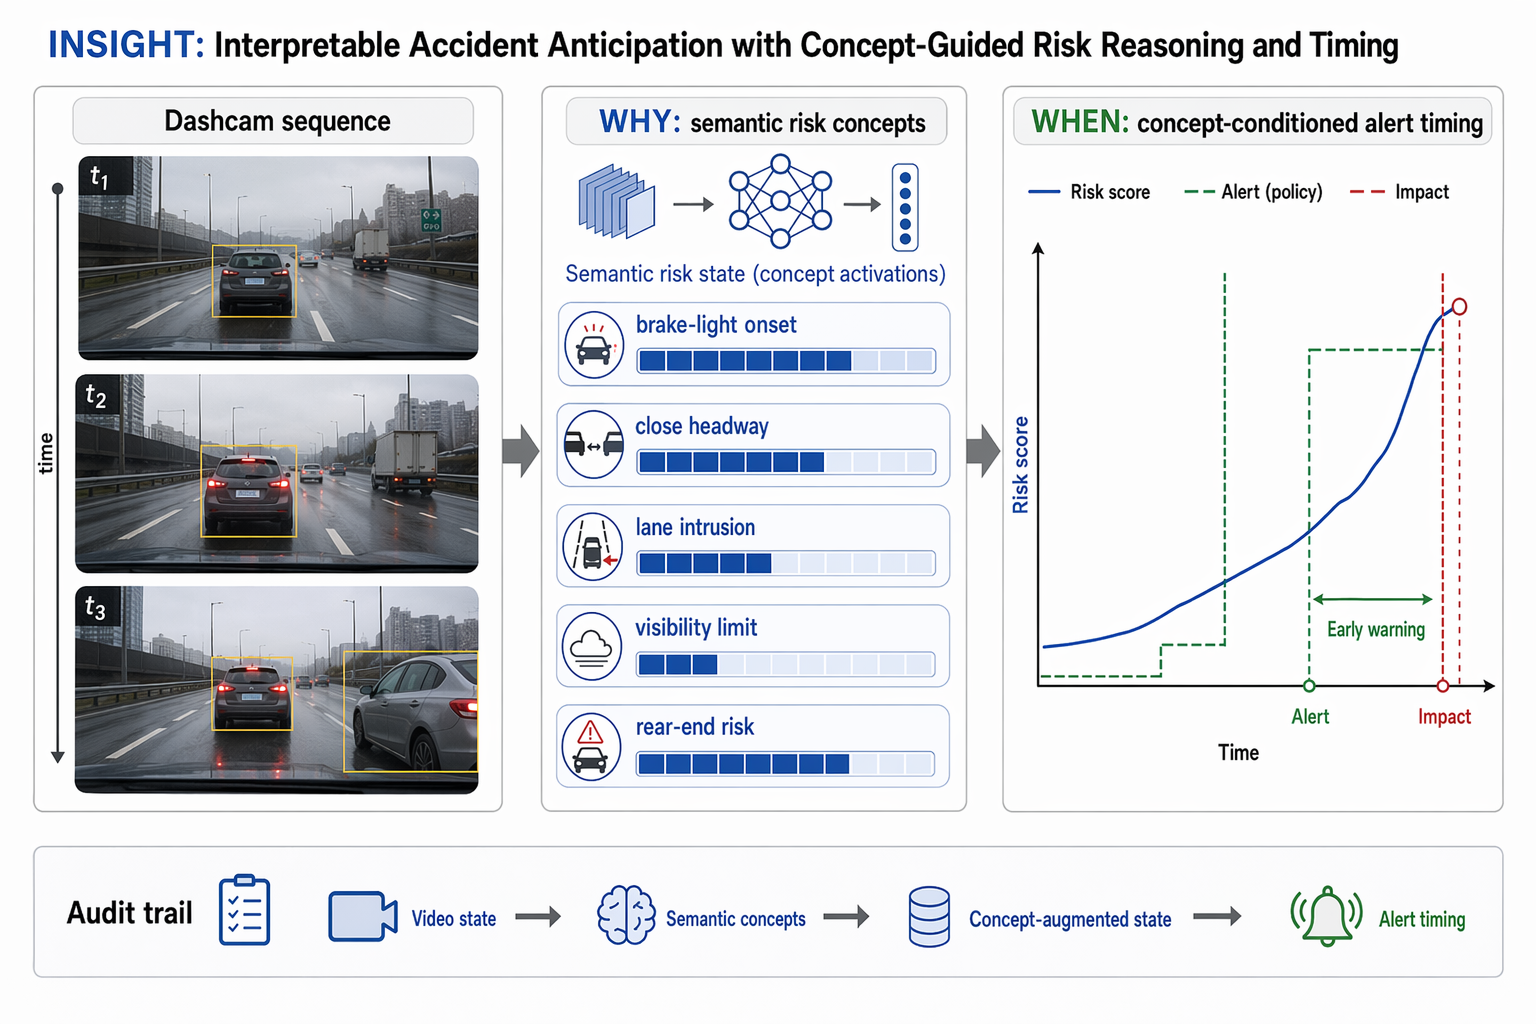
\includegraphics[width=0.985\textwidth]{../figures/insight_gpt_image2_teaser.pdf}
  \caption{\textbf{Schematic overview of \method{}.}
  \method{} builds an interpretable semantic risk state from video evidence,
  exposes \emph{why} risk is increasing through named concepts, and conditions
  \emph{when} to warn on that concept-augmented state. The dashcam panels are
  illustrative rather than evaluation evidence; real DAD case studies are
  reported in Figure~\ref{fig:multi}. The figure illustrates the intended link
  between semantic evidence (WHY) and concept-conditioned alert timing (WHEN)
  without treating the actor branch as a fully validated policy-level claim.}
  \label{fig:motivation}
\end{figure*}


\paragraph{What the field gets wrong.}
The recent literature has made impressive progress on Average Precision.
CCAF-Net~\citep{liu2025ccaf} reports 81.3\% AP on DAD,
and LATTE~\citep{ZHANG2025103173} reaches 89.7\%.
But these gains obscure two unresolved problems.

\textbf{First, existing methods are accuracy-optimal but timing-agnostic.}
Accident anticipation is usually formulated as binary classification with
cross-entropy loss.
This objective rewards confidence near the accident moment, where visual
evidence is strongest.
As a result, it systematically favours \emph{late certainty} over
\emph{early utility}.
In other words, the standard training objective is misaligned with the
real-world goal: every second of advance warning matters far more than a
small increase in probability immediately before impact.
The field has therefore optimised the wrong quantity.

\textbf{Second, the field lacks intrinsic dual-layer interpretability.}
A deployment-ready anticipation system must answer two distinct questions:
\emph{WHY is the scene dangerous?} and \emph{WHEN should the alert fire?}
Prior work addresses this only partially.
DRIVE~\citep{ref2} appends Grad-CAM after prediction---a post-hoc heatmap,
not a structural explanation.
W3AL~\citep{liao2024and} uses an LLM to verbalise accident location,
which is linguistic localisation rather than concept-level risk reasoning.
CRASH, DSTA, DAA-GNN, CCAF-Net, and LATTE provide no intrinsic
interpretability at all.
Few existing methods jointly explain both risk semantics (WHY)
and alert timing (WHEN) within the model itself.

\paragraph{Our central insight.}
The field has treated timing and interpretability as separate issues, but both
arise from the same modelling choice: framing accident anticipation as
classification rather than as semantic risk reasoning plus sequential timing
control. Once the decision state is defined as
$\mathbf{s}_t=[\mathbf{h}_t\|\mathbf{c}_t]$, with $\mathbf{c}_t$ containing
human-readable risk concepts, alert timing becomes conditioned on explicit
semantic evidence rather than on an opaque latent state alone. This view also
makes concept construction part of the method: in accident anticipation, a
generic visual vocabulary is often too noisy, while a fully manual ontology is
hard to scale. We therefore pair concept-conditioned timing control with a
reproducible pipeline for constructing risk concepts themselves.

\paragraph{\method{}: concept-augmented MDP state for dual-layer transparency.}
We propose \method{} (\textbf{In}terpretable \textbf{S}afety-\textbf{G}uided
accident anti\textbf{ci}pation via concep\textbf{t} bott\textbf{le}neck and
concept-aware actor-critic), a framework that couples a concept bottleneck,
concept-conditioned temporal modelling, and a timing-aware policy with a
reproducible risk-concept construction pipeline. Concretely, the model combines
(i) a concept discovery and polishing pipeline, (ii) the \cbm{} WHY layer,
(iii) the global \crs{} ranking, (iv) \cgta{} for concept-linked temporal
attention, (v) \tsd{} for anticipatory representation learning, and
(vi) \caac{} for concept-conditioned timing control.

The result is a jointly trained framework that couples an interpretable WHY
layer with a concept-conditioned timing mechanism, while grounding its semantic
interface in a reproducible ontology-construction pipeline.

\paragraph{Contributions.}
\begin{itemize}[leftmargin=1.4em,topsep=2pt,itemsep=1pt]
  \item We reframe accident anticipation as a \emph{concept-conditioned sequential decision problem} rather than binary classification with post-hoc explanation.
  \item We introduce a reproducible multimodal risk-concept construction pipeline and show through matched ontology comparisons that ontology choice changes the AP--mTTA operating point on DAD and A3D.
  \item We propose \method{}, which places semantic concepts directly in the decision state and thereby couples interpretable risk evidence with timing control.
  \item We present intervention evidence showing that concept edits can perturb downstream warning behaviour, while keeping policy-level claims scoped to the evidence currently available.
  \item We obtain 93.40\% AP / 4.90s mTTA on A3D and 68.19\% AP on DAD with a 30M-parameter model.
\end{itemize}

\section{Related Work}
\label{sec:related}

\paragraph{Traffic accident anticipation.}
The accident anticipation literature has focused primarily on improving
prediction accuracy from video. The seminal DSA-RNN~\citep{ref4} established
the DAD benchmark and showed that soft attention over detected objects enables
anticipation roughly 2\,s before impact. Subsequent work explored richer
interaction modelling, better spatio-temporal fusion, and larger-capacity
architectures. Examples include agent-centric risk assessment and risky-region
localisation~\citep{ref45}, uncertainty-aware relational reasoning~\citep{ref1},
adaptive learning for rare incidents~\citep{ref1}, dynamic spatio-temporal
attention~\citep{ref17}, graph-based interaction modelling~\citep{ref32,ref36,ref37},
and recent high-capacity fusion pipelines such as CRASH~\citep{liao2024crash},
CCAF-Net~\citep{liu2025ccaf}, and LATTE~\citep{ZHANG2025103173}. Recent work
has also begun to target timing more explicitly through temporal occurrence
prediction, risk propagation, and other formulations that model warning timing
more directly than a pure per-frame binary score. Other recent directions bring
language or textual supervision into anticipation, which is relevant to our use
of concept pseudo-labels even when the mechanism is not an explicit concept
bottleneck.

Despite their architectural diversity, most existing methods still optimize
anticipation mainly through prediction quality, with timing handled indirectly
through the shape of the confidence trajectory rather than through an explicit,
interpretable decision state. This has produced impressive AP numbers, but it
leaves two safety-critical gaps unresolved: the models are rewarded mainly for
being correct rather than early in a decision-theoretic sense, and the
internal evidence driving the alert remains largely latent.

\paragraph{Interpretability in accident anticipation.}
Table~\ref{tab:interp_comparison} (Experiments) makes the key point clear:
existing approaches, when they provide explanation at all, do so in ways that
remain external to the actual decision pathway. \citet{ref2} (DRIVE, MM'21) is
the closest prior work because it couples anticipation with reinforcement
learning and visual explanation. However, its Grad-CAM maps are still
\emph{post-hoc}: they are generated after prediction and do not constitute a
semantic state through which the decision is made. \citet{liao2024and}
(W3AL, MM'24) uses an LLM to verbalise accident location and timing, which is
interesting for description but fundamentally different from exposing a
human-auditable risk representation that directly controls the warning policy.
Other explanation-oriented studies remain similarly limited to heatmaps,
localisation, or auxiliary user-facing outputs~\citep{ref102,karim2023attention}.

This distinction matters. In a safety setting, an explanation is most useful
when it is not merely attached to a decision but structurally involved in the
decision itself. \method{} is designed around exactly this requirement: the
concept activations are not generated after the alert, but are part of the
forward path that produces it. This is why we emphasise \emph{intrinsic}
WHY/WHEN interpretability rather than post-hoc explanation quality alone.

\paragraph{Actor-Critic for temporal decisions.}
\citet{sutton2018reinforcement} establish the Actor-Critic framework.
\citet{ref2} (DRIVE) applies REINFORCE to learn a spatial attention
policy for object selection, using RL as a training signal rather than
for optimizing the final alert rule. Recent timing-oriented accident
anticipation methods have also explored temporal occurrence prediction and
related formulations without exposing an explicit semantic decision state. The
main distinction of \caac{} in the current paper is therefore not simply that
it uses RL, but that the state $\mathbf{s}_t=[\mathbf{h}_t\|\mathbf{c}_t]$
contains concept activations and thus provides a direct route from semantic
risk evidence to timing control.

\paragraph{Concept Bottleneck Models and knowledge distillation.}
Concept Bottleneck Models (CBMs) constrain predictions through interpretable
bottlenecks~\citep{ref102}, offering human-readable intermediate representations
that support user intervention.
Applying CBMs to \emph{video} accident anticipation is non-trivial:
concepts must be dynamic across frames, and temporal dependencies must be
preserved through the bottleneck.
\method{} addresses both challenges through \cgta{} (linking temporal
attention to concept dynamics) and the \caac{} state design (placing
concepts directly inside the MDP state).

For concept supervision, \method{} leverages CLIP~\citep{radford2021learning},
which provides rich semantic visual representations from natural language
supervision and enables pseudo-labelling of 837 traffic-relevant concepts
without manual annotation. This choice should be read as a practical semantic
bootstrap rather than as a claim that the resulting pseudo-concepts are fully
noise-free; in the current paper, the strongest support for the concept layer
comes from architectural transparency, ontology analysis, and downstream
ablation evidence rather than from a standalone concept-label benchmark.
The \tsd{} component distils CLIP future-frame features into current
representations, providing anticipatory semantic grounding inspired by
self-predictive representation learning~\citep{fang2022traffic}.

\section{\method: Dual-Layer Interpretable Accident Anticipation}
\label{sec:method}

We present \method{}, a unified framework for intrinsically interpretable
accident anticipation. Figure~\ref{fig:framework} gives an overview.
We describe each component in order of information flow.

\begin{figure*}[t]
  \centering
  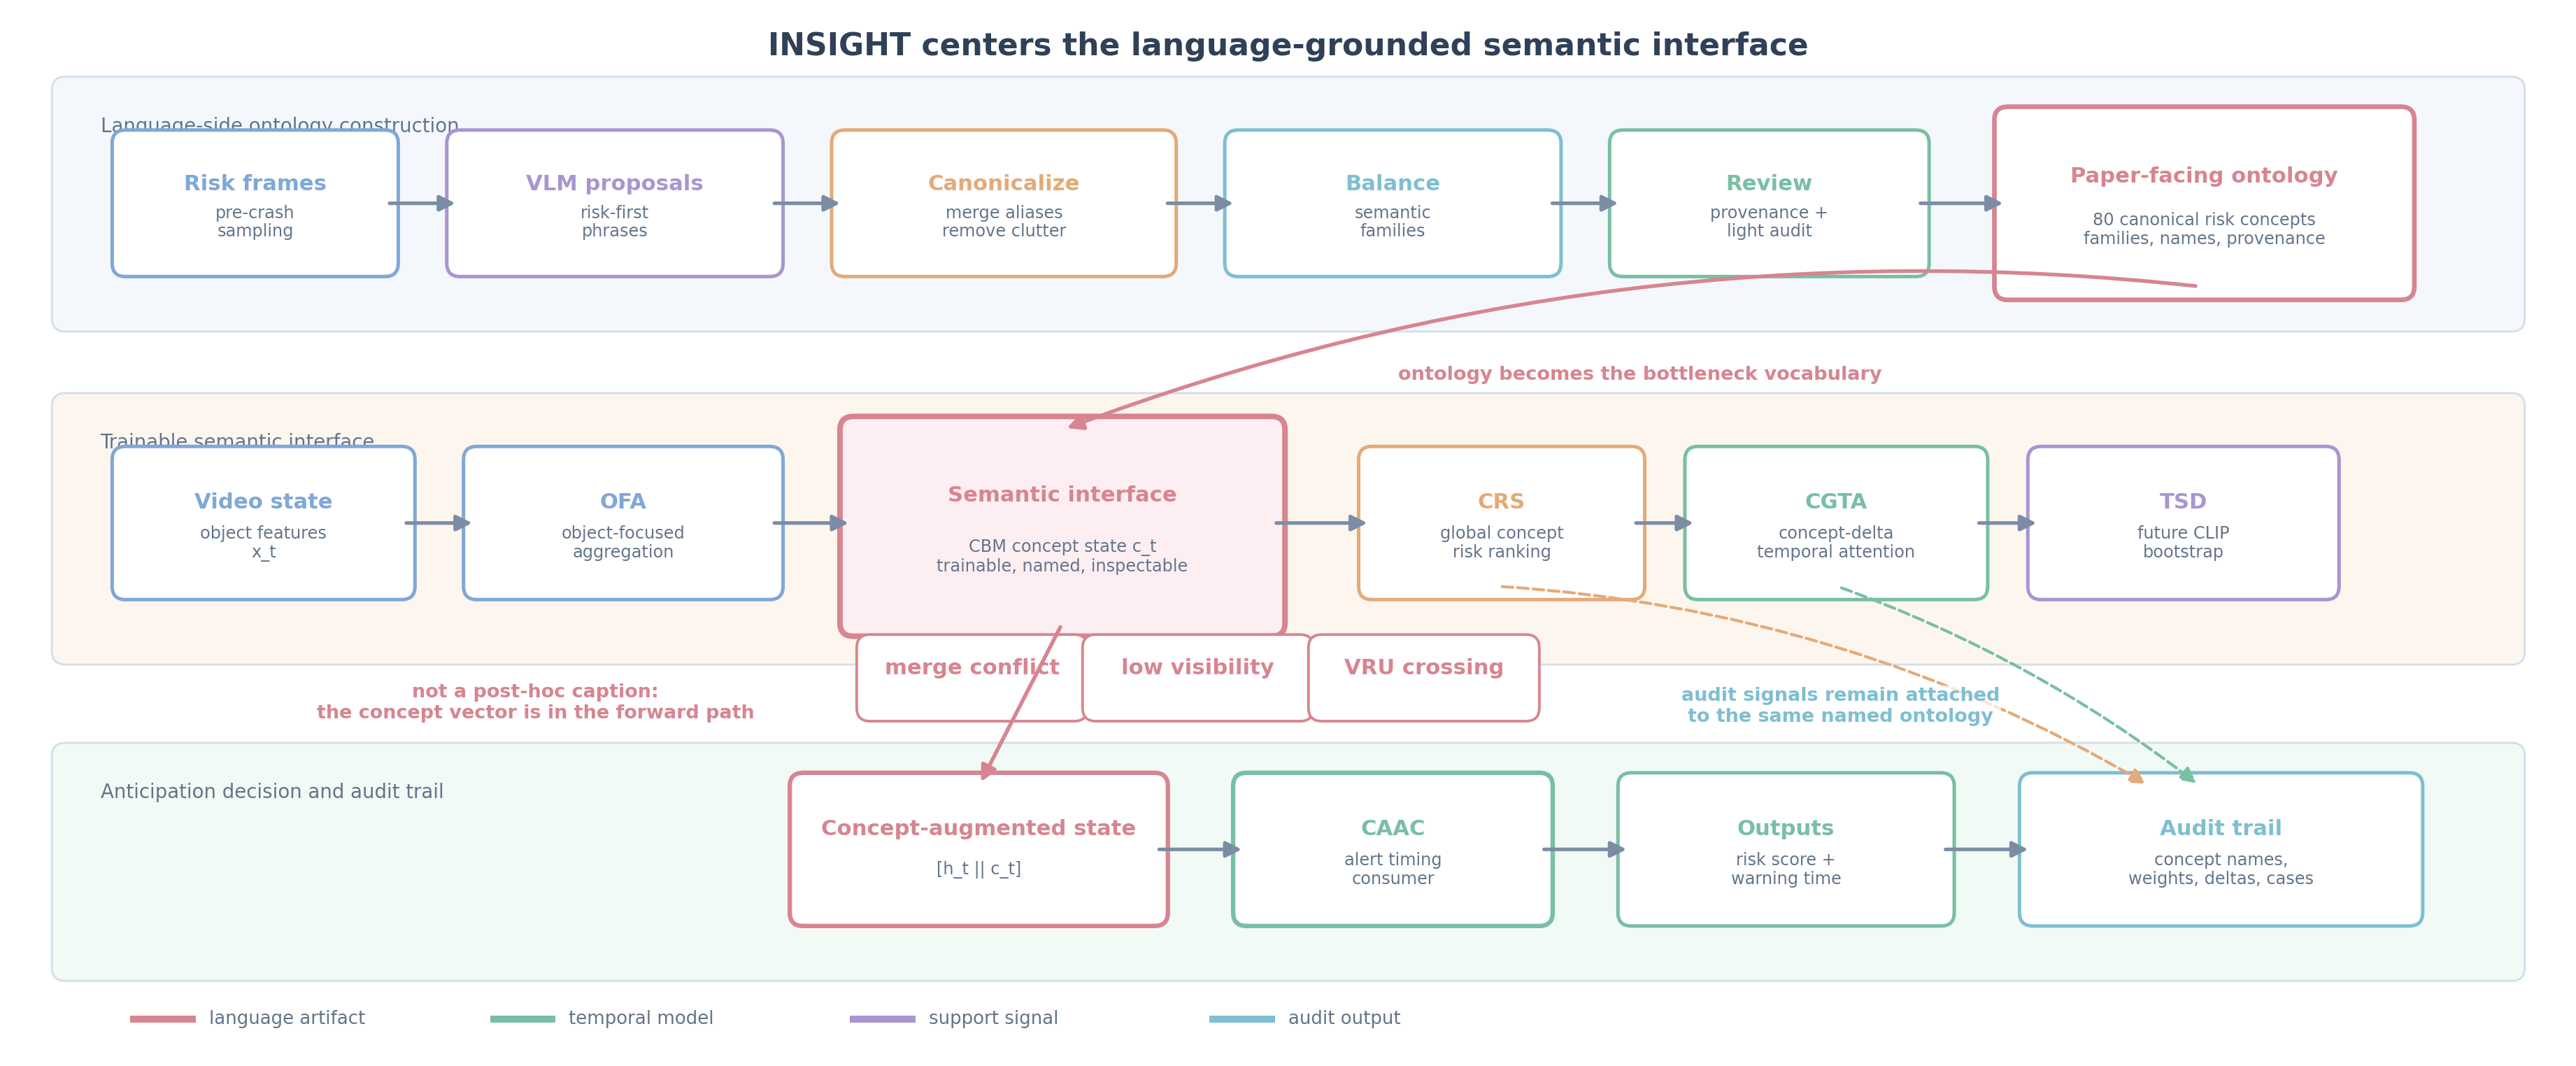
\includegraphics[width=\textwidth]{../figures/insight_framework.pdf}
  \caption{\textbf{INSIGHT framework overview.} Per-frame information flows
  left-to-right through five modules. The \textcolor{red}{\textbf{WHY layer}}
  (CBM) maps object features to $K{=}837$ interpretable risk concepts
  $\mathbf{c}_t$. The \textcolor{green!50!black}{\textbf{WHEN layer}}
  (CAAC) uses concept-augmented state $\mathbf{s}_t=[\mathbf{h}_t\|\mathbf{c}_t]$
  to optimise alert timing via a time-remaining reward. CRS provides an
  auditable per-concept risk ranking; CGTA links temporal attention to
  concept dynamics; TSD distils CLIP future features for anticipatory
  representations. The dashed arc (CBM$\to$CAAC) denotes the concept
  state pathway that makes every alert decision concept-traceable by construction.}
  \label{fig:framework}
\end{figure*}

\subsection{Problem Formulation}

Given a dashcam video $\{\mathbf{x}_t\}_{t=1}^T$ with
$\mathbf{x}_t \in \mathbb{R}^{N \times D}$
($N{=}19$ detected objects, $D{=}4096$ VGG16~\citep{ref31} ROI features),
a binary label $y \in \{0,1\}$, and time-of-accident $\tau$,
\method{} is motivated by the following idealised objective:
\begin{equation}
  \max_{\theta}\; \mathbb{E}[\mathrm{TTA}]
  \quad \text{s.t.} \quad \mathrm{AP}(\theta) \geq \mathrm{AP}_{\text{base}},
  \label{eq:objective}
\end{equation}
where $\mathrm{TTA} = (\tau - t^*)/\mathrm{fps}$ and
$t^* = \min\{t : \pi_\theta(\mathrm{alert}\mid\mathbf{s}_t) \geq 0.5\}$
is the first alert frame.
This objective should be read as a \emph{motivational target} rather than as
a literal constrained solver used in optimization. In practice, we implement a
surrogate multi-loss training objective that balances classification,
concept supervision, timing control, and anticipatory representation learning,
and we evaluate the resulting AP--mTTA trade-off empirically.

\subsection{Overview}

\paragraph{Design intuition.}
The central design principle of \method{} is simple:
\emph{concepts should not merely explain the prediction after the fact;
they should participate directly in the decision process itself}.
To achieve this, \method{} first extracts an interpretable concept state,
then uses those concepts to modulate temporal attention, risk scoring,
and finally the Actor-Critic timing policy.
This tight coupling between semantics and sequential decision-making
is what enables simultaneous WHY and WHEN transparency.

The per-frame forward pass is:
\begin{align*}
  \mathbf{x}_t
  &\xrightarrow{\text{OFA}} \mathbf{o}_t
  \xrightarrow{\cbm} (\mathbf{c}_t,\mathbf{e}_t)
  \xrightarrow{\crs} \rho_t \\
  &\xrightarrow{\cgta} \mathbf{g}_t
  \xrightarrow{\text{GRU}} \mathbf{h}_t
  \xrightarrow{\caac} (p_t, a_t, V_t).
\end{align*}
The key design choice is that the \caac{} MDP state
$\mathbf{s}_t = [\mathbf{h}_t \| \mathbf{c}_t]$ explicitly includes
concept activations, making every alert-timing decision concept-traceable
by construction.

\subsection{Object-Focused Aggregation}

The $N$ object features per frame are aggregated by an Object-Focused
Attention (OFA) module:
\begin{align}
  \alpha^n_t &= \mathrm{softmax}_n\bigl(\mathbf{w}_a^\top
    \tanh(\mathbf{W}_o \mathbf{x}^n_t)\bigr), \\
  \mathbf{o}_t &= \sum_{n=1}^N \alpha^n_t\,\mathbf{W}_f \mathbf{x}^n_t
    \in \mathbb{R}^h.
\end{align}

\subsection{Concept Ontology Discovery and Adjudication}

\paragraph{Why ontology construction matters.}
A concept bottleneck is only as good as its vocabulary.
In accident anticipation, a generic traffic word list is often too broad,
while a fully manual ontology is difficult to scale and easy to bias toward
researcher priors. We therefore treat concept construction itself as part of
our method rather than as an external preprocessing detail. The goal is not to
generate visually descriptive tags, but to produce \emph{trainable,
auditable, and intervention-ready risk primitives} that can serve as the
semantic interface for the WHY layer.

\paragraph{Stage 1: frame mining.}
We first build a frame manifest from positive accident videos by sampling
pre-crash frames that exhibit diverse traffic geometries, actor interactions,
and visibility conditions. This step avoids querying a multimodal model on all
video frames while still covering the semantic support of accident precursors.
Importantly, the sampling policy is risk-oriented: frames are chosen to expose
emerging hazards rather than merely static scene diversity.

\paragraph{Stage 2: multimodal risk concept discovery.}
Given sampled frames, a multimodal language model proposes candidate concepts,
risk factors, and coarse semantic families. Our prompts explicitly ask for
\emph{risk-first} concepts---such as cut-in behaviour, brake-light onset,
visibility degradation, or closing distance---rather than generic scene
captions. The raw output is therefore a noisy but high-recall pool of accident
precursor phrases rather than a polished ontology.

\paragraph{Stage 3: risk-first refinement.}
We then refine the raw pool by prioritising causal or precursor-like factors,
filtering obvious background clutter, merging near-duplicates, and normalising
phrasing toward concise risk primitives. This stage is intentionally asymmetric:
it prefers under-specification over over-fragmentation, because downstream
training benefits more from stable and reusable primitives than from dozens of
near-synonymous micro-concepts.

\paragraph{Stage 4: ontology polishing, family balancing, and human review.}
The final step is no longer just canonical renaming. Starting from the large-vocabulary
academic pool, we perform a dedicated polishing pass that audits family coverage,
consolidates high-priority duplicate clusters (especially visibility, pedestrian-crossing,
and merge-related concepts), normalises naming into short canonical risk phrases,
and then applies a very-light human review over every retained concept.
This transforms the ontology from a high-recall phrase pool into a
\emph{paper-ready semantic interface}: compact enough to present clearly,
rich enough to preserve major accident precursor families, and explicit enough to
support intervention analysis, family-level auditing, and appendix-level ontology reporting.
Figure~\ref{fig:concept_pipeline} visualises the end-to-end process, and
Figures~\ref{fig:concept_evolution} and~\ref{fig:concept_case_study} show how
noisy phrase sets are converted into canonical trainable concepts.

\begin{figure*}[t]
  \centering
  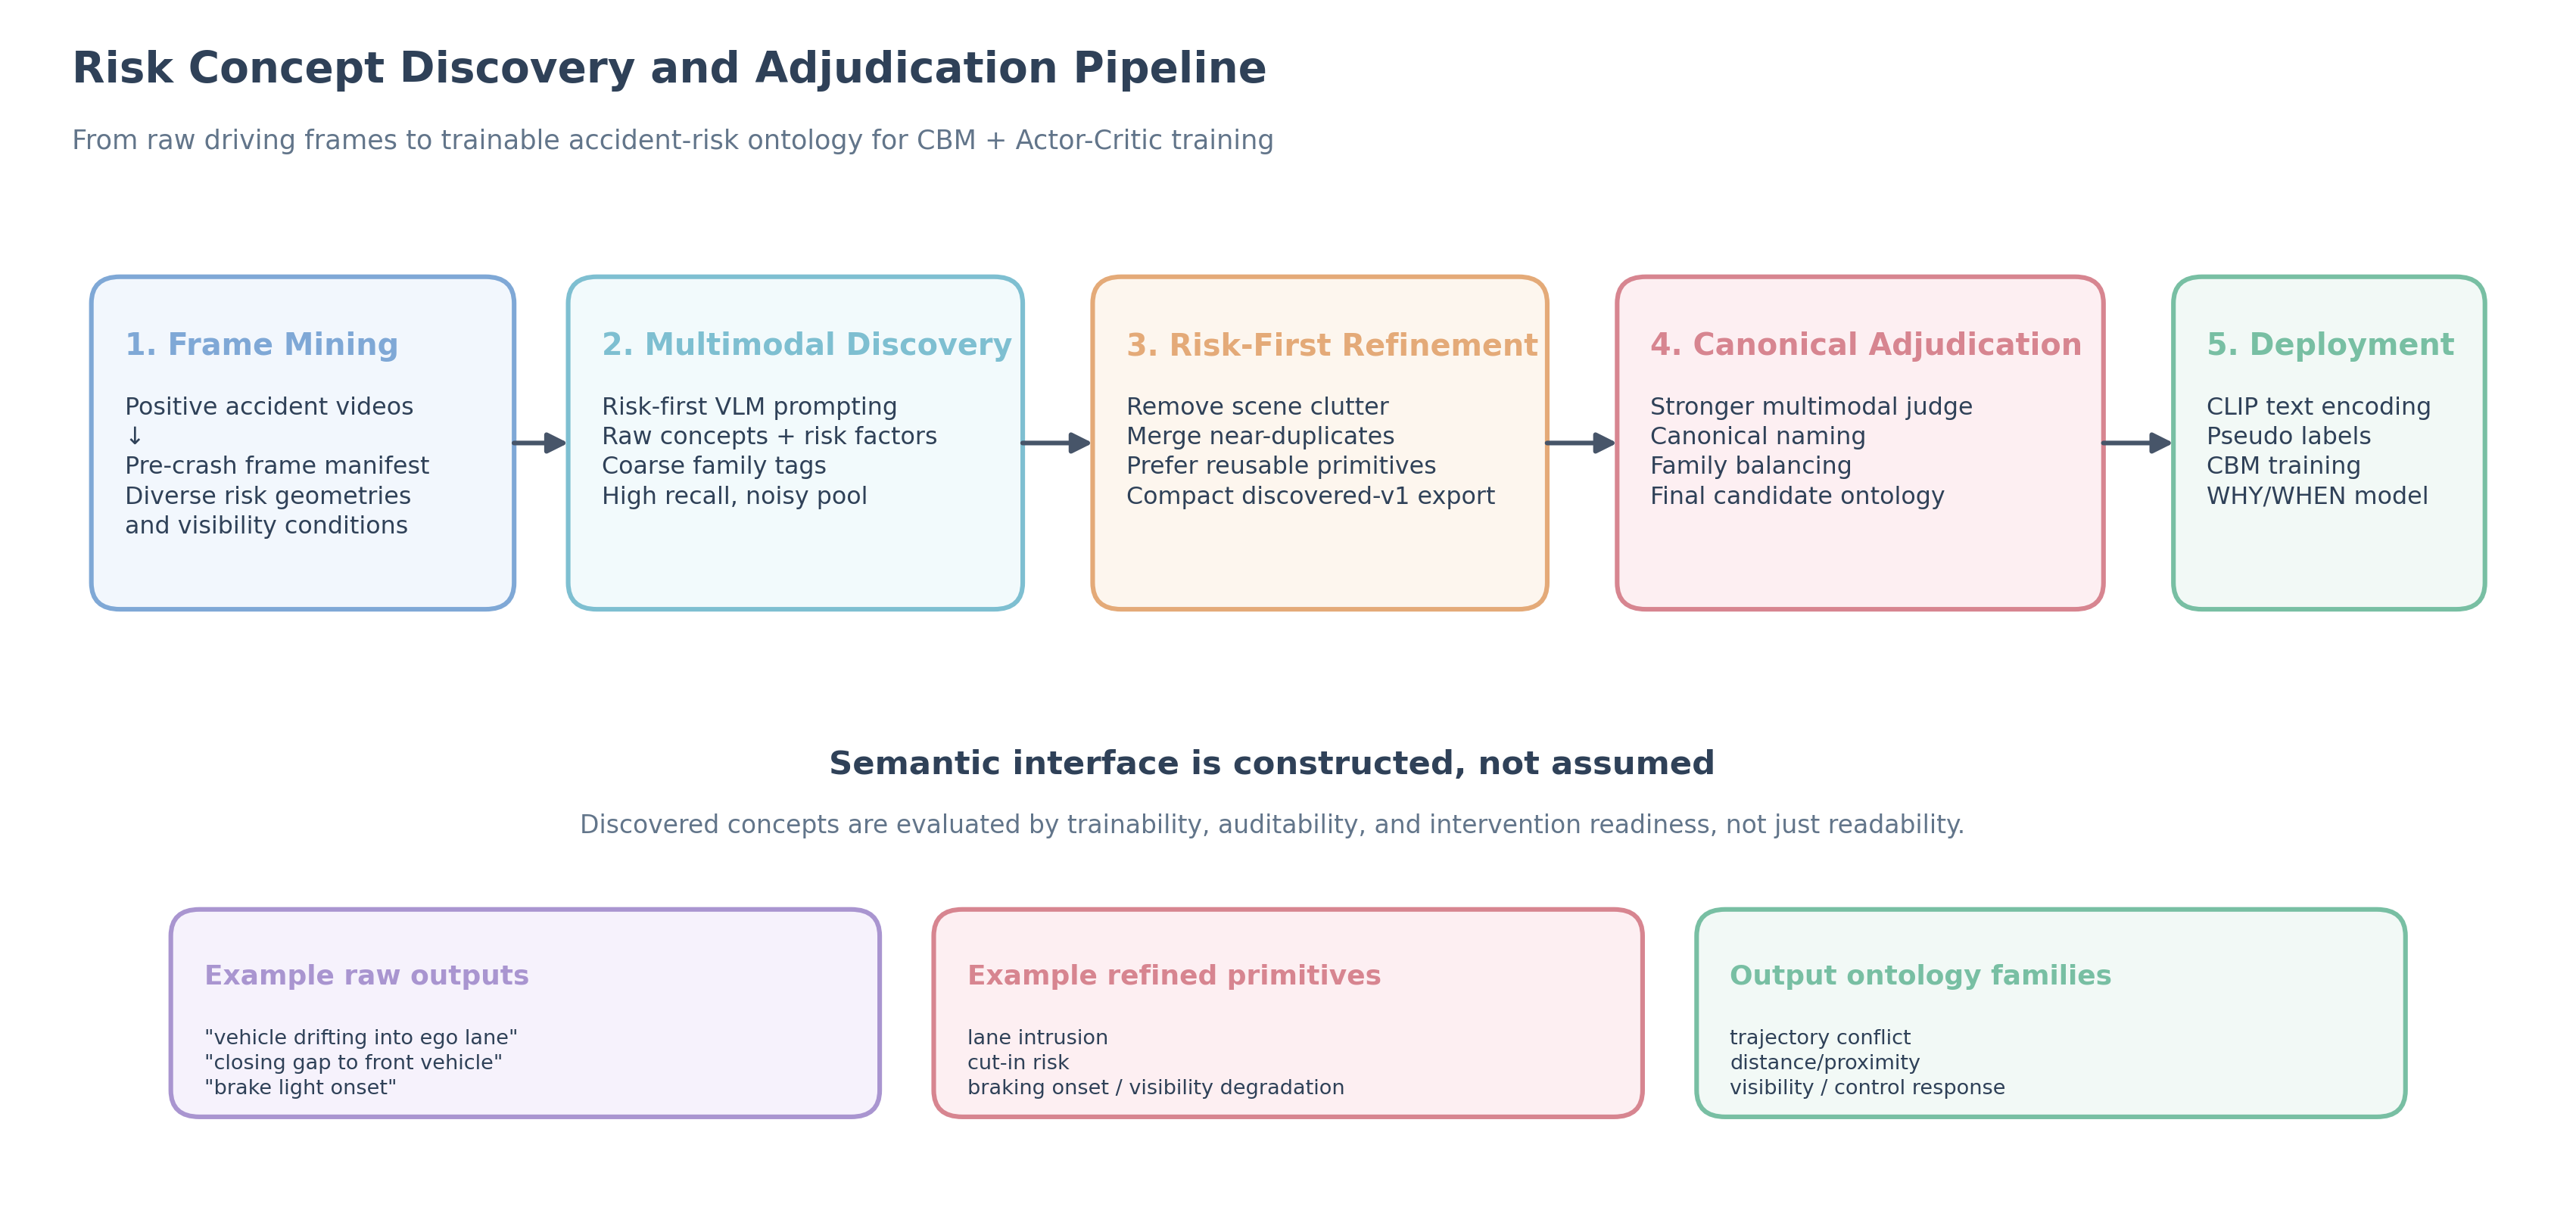
\includegraphics[width=0.98\textwidth]{../figures/insight_fig_concept_pipeline.pdf}
  \caption{\textbf{End-to-end concept ontology construction pipeline.}
  Starting from sampled pre-crash driving frames, the pipeline performs
  multimodal risk-concept discovery, risk-first refinement, duplicate-cluster
  consolidation, family balancing, and light human review to produce a final
  trainable ontology for the concept bottleneck. This figure clarifies that the
  ontology is a reproducible methodological component rather than a hidden fixed
  vocabulary assumption.}
  \label{fig:concept_pipeline}
\end{figure*}

\paragraph{What the final ontology is designed to optimise.}
The final discovered ontology is not selected only for lexical cleanliness.
It is designed to jointly optimise four properties: (i)~semantic plausibility,
(ii)~family coverage, (iii)~trainability in the downstream CBM+Actor--Critic
pipeline, and (iv)~paper-level auditability. This design choice matters.
A compact ontology that is easy to read but too narrow to train well is not
useful; conversely, a broad ontology that trains well but remains lexically noisy
is difficult to defend as a scientific semantic interface.
Our polishing stage therefore treats ontology construction as a structured model-design
problem rather than a cosmetic prompt-engineering step.

\paragraph{Deployment into the CBM.}
The output of the pipeline is a text ontology that can be encoded with CLIP and
used immediately for pseudo concept supervision and concept bottleneck
training. This is a key design choice: concept discovery is evaluated not only
by semantic plausibility, but also by whether the resulting ontology survives
contact with downstream learning. In our experiments, discovered concept sets
are therefore treated as first-class trainable assets rather than appendix-only
qualitative artifacts. The final paper-ready concept set is additionally stored
with family metadata, merge provenance, and exhaustive per-concept human-review
notes, making the ontology itself a reproducible research asset.

\subsection{Concept Bottleneck Module (CBM)}

\paragraph{Why a concept bottleneck?}
A raw hidden state may be predictive, but it is not auditable.
The \cbm{} explicitly constrains the model to represent each frame
through a set of human-readable risk concepts.
This creates a semantic interface between the visual backbone and the
decision policy: if the system predicts danger, one can inspect which
concepts were active and by how much.
The downstream consequence is crucial: once risk is represented in a
concept space, both prediction and decision-making become auditable at
a granularity safety engineers can reason about.

The \cbm{} maps aggregated features to $K$ human-interpretable
risk concepts, where $K$ depends on the ontology used in a given run
($K{=}837$ for the historical full vocabulary and $K{=}80$ for the current
paper-ready discovered ontology):
\begin{align}
  \mathbf{c}_t &= \sigma(\mathbf{W}_c \mathbf{o}_t + \mathbf{b}_c)
    \in [0,1]^K, \\
  \mathbf{e}_t &= \mathrm{LayerNorm}(\mathbf{W}_d \mathbf{c}_t + \mathbf{b}_d)
    \in \mathbb{R}^h.
\end{align}
Concept activation $c_{t,k}$ directly quantifies how strongly risk
factor $k$ is present in frame $t$---this is the \textbf{WHY-layer}
explanation.

\paragraph{Auxiliary concept supervision.}
CLIP-derived pseudo concept labels $\hat{\mathbf{c}}_t \in \{0,1\}^K$
are obtained via cosine similarity between CLIP image features and
concept text embeddings~\citep{radford2021learning}. For each frame,
we mark concept $k$ as positive if its similarity score falls in the
frame-wise top-$m$ set ($m{=}3$ in our main runs) and negative otherwise:
this gives a sparse binary target that avoids introducing an additional
global threshold hyperparameter into the main training recipe.
\begin{equation}
  \mathcal{L}_{\text{aux}}
  = \frac{1}{K}\,\mathrm{BCE}(\mathbf{c}_t,\,\hat{\mathbf{c}}_t).
\end{equation}

\subsection{Concept Risk Score (CRS)}

Learnable per-concept risk weights $\mathbf{w}_{\text{risk}} \in \mathbb{R}^K$
produce an auditable scalar safety signal:
\begin{equation}
  \rho_t = \sigma(\mathbf{w}_{\text{risk}})^\top \mathbf{c}_t \in \mathbb{R}.
  \label{eq:crs}
\end{equation}
Unlike attention weights, $\mathbf{w}_{\text{risk}}$ is a global parameter
shared across all frames: safety engineers can inspect the ranked concept
list and override individual entries for jurisdiction-specific deployment.

\subsection{Concept-Guided Temporal Attention (CGTA)}

\paragraph{Why concept-guided temporal attention?}
Standard temporal attention operates on hidden features and often lacks
a clear semantic interpretation.
\cgta{} instead uses \emph{concept deltas} as its query signal:
when a risk concept suddenly rises, the model should look back to the
frames that caused that rise.
This transforms temporal attention from a generic sequence mechanism
into a concept-linked temporal audit trail.
The consequence is that rising risk can be traced not only to a concept,
but also to the historical evidence that caused that concept to activate.

\cgta{} uses concept activation deltas as temporal attention queries,
linking temporal focus directly to concept dynamics. At frame $t$, the
attention index $s$ ranges over the available history $1,\dots,t-1$:
\begin{align}
  \Delta\mathbf{c}_t &= \mathbf{c}_t - \mathbf{c}_{t-1}, \\
  \alpha_{t,s} &=
    \frac{\exp\bigl((\mathbf{W}_Q\Delta\mathbf{c}_t)^\top
      (\mathbf{W}_K\mathbf{h}_s)/\sqrt{h}\bigr)}
    {\sum_{s'=1}^{t-1}\exp\bigl((\mathbf{W}_Q\Delta\mathbf{c}_t)^\top
      (\mathbf{W}_K\mathbf{h}_{s'})/\sqrt{h}\bigr)}, \\
  \mathbf{g}_t &= \lambda_{\text{gate}}\sum_{s=1}^{t-1}\alpha_{t,s}\mathbf{W}_V\mathbf{h}_s
    + (1-\lambda_{\text{gate}})\mathbf{h}_{t-1},
\end{align}
where $\lambda_{\text{gate}} = \sigma(w_{\text{gate}})$ is learnable.
When concept $k$ spikes at frame $t$, $\alpha_{t,s}$ highlights the past
frames that led to the spike, providing a temporal audit trail.

\subsection{Temporally Shifted Distillation (TSD)}

\paragraph{Why future-frame distillation?}
A strong anticipation model should encode not only what is visible now,
but also what is likely to happen next.
\tsd{} encourages the current representation to align with CLIP features
from a short future horizon, injecting anticipatory semantics into the
hidden state without requiring a heavy video-pretrained teacher.
The practical consequence is that the representation becomes predictive
rather than merely descriptive: it encodes where the scene is headed,
not just what the current frame contains.

\tsd{} distils CLIP future-frame features into current representations,
encouraging anticipatory semantics without video-pretrained teachers:
\begin{equation}
  \mathcal{L}_{\text{TSD}}
  = \bigl\|\mathbf{W}_{\text{TSD}}\mathbf{o}_t
    - \mathrm{sg}(\mathbf{f}^{\text{CLIP}}_{t+\delta})\bigr\|_2^2,
  \label{eq:tsd}
\end{equation}
where $\mathrm{sg}(\cdot)$ is stop-gradient and $\delta{=}5$ frames.

\subsection{Concept-Aware Actor-Critic (CAAC)}

\paragraph{Why Actor-Critic?}
Accident anticipation is not purely a classification problem;
it is a sequential decision problem with asymmetric temporal cost.
Issuing the correct alert 0.1\,s before impact is far less useful
than issuing it 2\,s earlier.
Actor-Critic provides the right optimisation target: a reward that
can be made explicitly proportional to time remaining before accident.
By concatenating concepts into the MDP state, the resulting timing
policy is not only optimal in expectation, but also interpretable.
The consequence is a policy that can learn to alert \emph{before}
probability peaks, while still exposing the semantic evidence behind
that early decision.

\paragraph{Why the dual-layer decomposition is structurally useful.}
The benefit of splitting the model into a WHY layer and a WHEN layer is not
just interpretive clarity; it changes the optimisation problem itself.
If risk evidence is represented only in an opaque latent state, then the model
must jointly discover \emph{what} matters and \emph{when} to act in one
entangled space. By introducing an explicit concept state $\mathbf{c}_t$ and
placing it directly into the decision state $\mathbf{s}_t$, \method{} instead
factorises the problem into semantic evidence estimation and timing control.
This factorisation makes intervention meaningful: a perturbation on a risk
concept induces a perturbation on the policy state itself, so concept edits can
in principle alter the alert timing rather than merely explain it after the
fact. This is the formal reason our intervention analysis is architecturally
relevant rather than decorative.

\paragraph{State.}
The MDP state concatenates GRU hidden state with concept activations:
\begin{equation}
  \mathbf{s}_t = [\mathbf{h}_t \| \mathbf{c}_t] \in \mathbb{R}^{h+K}.
  \label{eq:state}
\end{equation}
Because $\mathbf{c}_t$ is in the state, the Actor's policy is directly
conditioned on concept activations---every alert-timing decision is
concept-traceable by design. This is the \textbf{WHEN-layer explanation}.

\paragraph{Actor and Critic.}
\begin{align}
  \pi(a_t \mid \mathbf{s}_t)
    &= \mathrm{Softmax}(\mathbf{W}_\pi \mathbf{s}_t + \mathbf{b}_\pi),
    \quad a_t \in \{\text{wait},\text{alert}\}, \\
  V(\mathbf{s}_t)
    &= \mathbf{w}_V^\top \tanh(\mathbf{W}_{V_1} \mathbf{s}_t).
\end{align}

\paragraph{Concept-aware reward and episode definition.}
Each video constitutes one finite-horizon episode of length $T$.
At every frame the agent chooses $a_t\in\{\text{wait},\text{alert}\}$,
but only the \emph{first} alert is operationally relevant: once the first
alert is emitted, the rollout terminates and no further actions are taken.
If a positive video reaches frame $\tau$ without any alert, we assign a single
miss penalty at that terminal step. If a negative video emits an alert at any
frame, the episode also terminates immediately with a false-alarm penalty.
The reward incentivises \emph{early} correct alerts via temporal urgency:
\begin{equation}
  \mathfrak{r}_t = \begin{cases}
    \lambda_r \cdot \dfrac{\tau - t}{\tau} \cdot (1 + \beta\, b_t)
      & \text{first alert on a positive sample with } t < \tau \\[4pt]
    -\lambda_p & \text{first alert on a negative sample} \\[4pt]
    -\lambda_p & \text{positive sample reaches } \tau \text{ without alert} \\[4pt]
    +\varepsilon & \text{intermediate wait action before termination.}
  \end{cases}
  \label{eq:reward}
\end{equation}
where $b_t = \sigma(\mathbf{w}_b^\top\mathbf{c}_t)$ is a learnable
concept bonus, $\lambda_r{=}5.0$, $\lambda_p{=}0.5$, $\beta{=}0.5$,
$\varepsilon{=}0.1$. The factor $\tfrac{\tau-t}{\tau}$ is the
\emph{temporal urgency}: earlier correct alerts receive higher reward,
directly favouring larger TTA.

\paragraph{Actor-Critic loss and inference coupling.}
Let $A_t = R_t - V(\mathbf{s}_t)$ be the advantage and
$R_t = \sum_{t'\geq t}\gamma^{t'-t}\mathfrak{r}_{t'}$ the discounted return
($\gamma{=}0.95$). The AC loss is:
\begin{align}
  \mathcal{L}_{\text{AC}}
  &= -\mathbb{E}_t[\log\pi(a_t\mid\mathbf{s}_t)\,A_t] \nonumber\\
  &\quad+ \lambda_V \mathbb{E}_t[(V(\mathbf{s}_t)-R_t)^2]
  - \lambda_H \mathcal{H}[\pi(\cdot\mid\mathbf{s}_t)],
  \label{eq:ac_loss}
\end{align}
with $\lambda_V{=}0.1$, $\lambda_H{=}0.005$.
During training, the classifier head $p_t$ and the policy head
$\pi(\text{alert}\mid\mathbf{s}_t)$ are optimized jointly through the shared
backbone and concept state. In the current paper, the first alert frame $t^*$
reported for AP/mTTA evaluation is defined from the classifier trajectory
$p_t$ rather than from the archived actor probability, because the classifier
branch is the reliable signal in all reported headline lines whereas the actor
branch is only partially validated in the archived intervention/timing package.
The policy head is therefore best interpreted here as a concept-conditioned
training signal and architectural timing mechanism whose full standalone
policy-level evaluation remains incomplete.

\subsection{Total Training Objective}

\paragraph{Training principle.}
The overall objective balances four competing requirements:
classification accuracy, semantic interpretability, temporal decision
quality, and anticipatory representation learning.
The warmup-and-ramp schedule is essential here: if the Actor--Critic
loss dominates too early, the model learns unstable policies before
the concept space has become semantically meaningful.
We therefore let the concept bottleneck stabilise first, then gradually
increase the weight of sequential decision optimisation.
The consequence is a more semantically coherent concept space and a more
stable policy-learning phase, which empirically improves both AP and mTTA.
The schedule described below is the shared default recipe; dataset-specific
variants used in individual tables are summarised explicitly in the experiments
section so that readers can map each reported result to its exact protocol.

The full loss combines classification, concept supervision, AC, and TSD:
\begin{equation}
  \mathcal{L}
  = \mathcal{L}_{\text{CE}}
  + \lambda_{\text{aux}}\,\mathcal{L}_{\text{aux}}
  + \lambda_{\text{AC}}\,\mathcal{L}_{\text{AC}}
  + \lambda_{\text{TSD}}\,\mathcal{L}_{\text{TSD}},
  \label{eq:total_loss}
\end{equation}
where $\lambda_{\text{aux}}{=}1.0$, $\lambda_{\text{AC}}$ is ramped
from $0$ to $1$ over epochs 20--50 (warmup then CBM ramp), and
$\lambda_{\text{TSD}}{=}0.1$. The warmup prevents AC from disrupting
early concept learning---analogous to the warmup schedule in
semi-supervised learning~\citep{fang2022traffic}.

\subsection{Design Rationale and Complexity Notes}
\label{sec:theory}

\paragraph{Complexity.}
The per-frame forward pass of \method{} has time complexity
$\mathcal{O}(NDh + Kh + h^2 + Kh)$, where the dominant costs are the
GRU recurrence $\mathcal{O}(h^2)$ and the concept-dependent projections
$\mathcal{O}(Kh)$. With $h{=}256$ and $K{=}837$, the raw CBM-related
$Kh$ term is numerically larger than $h^2$; the correct takeaway is therefore
not that the CBM is asymptotically smaller than the GRU, but that both remain
modest at the scale of our 30M-parameter model and do not dominate end-to-end
runtime in practice.

\paragraph{Structural role of concept-conditioned intervention.}
Let $\Delta\mathbf{c}\in\mathbb{R}^K$ be a concept edit applied to a
pre-crash window $[t_1, t_2]$. The perturbed MDP state becomes
$\mathbf{s}'_t = [\mathbf{h}_t\|\mathbf{c}_t + \Delta\mathbf{c}]$.
This observation does \emph{not} prove that a trained policy will respond
monotonically or strongly to every such edit. What it does establish is the
architectural precondition for intervention analysis: concept edits act on the
same semantic state that feeds the downstream timing mechanism.
state actually consumed by the policy rather than on a post-hoc explanation
channel. For this reason, the intervention experiments in
Section~\ref{app:intervention} should be interpreted as empirical tests of a
structurally intervenable interface, not as consequences of a formal monotonicity
guarantee.

\section{Experiments}
\label{sec:experiments}

\subsection{Experimental Setup}

\paragraph{Datasets.}
\textbf{DAD}~\citep{ref4}: 1,750 dashcam videos (620 accident,
1,130 non-accident) from six Taiwanese cities, split 1,280/450
train/test. Videos are 5\,s at 20\,fps (100 frames).
\textbf{A3D}~\citep{liao2024crash}: 1,199 videos (960/239) at 10\,fps,
100 frames, spanning diverse East Asian urban accident types.

\paragraph{Metrics.}
\textbf{AP}: area under the precision-recall curve.
\textbf{mTTA}: mean lead time between first issued alert and annotated
accident onset over correctly anticipated positives.
\textbf{TTA@R80} / \textbf{P@R80}: TTA and precision at 80\% recall.

\paragraph{Implementation details.}
VGG16~\citep{ref31} ROI features ($D{=}4096$, $N{=}19$ objects per frame).
For the full historical vocabulary we use $K{=}837$ concepts; for discovered
ontologies, $K$ is the size of the corresponding compact concept set.
AdamW with learning rate $3{\times}10^{-4}$, cosine decay, batch size 16,
and a 150-epoch schedule with 15 epochs of Actor--Critic warmup followed by a
20-epoch CBM ramp in the shared comparison runs. For DAD, our strongest current
submission result additionally uses a lightweight curriculum-stabilized variant
that delays the concept loss in the earliest stage before gradually ramping in
concept supervision. This improves stability on DAD while keeping the test
protocol and model family unchanged. For concept-set comparison experiments, we
keep the training recipe fixed and vary only the ontology source and concept
count, allowing us to attribute changes in performance to the semantic
interface rather than to optimizer choices.

\paragraph{Result reporting protocol.}
We separate \emph{canonical headline runs} from \emph{controlled support analyses},
but we do not select checkpoints by test-set performance. For each reported
training line, the paper uses a pre-specified evaluation snapshot: either the
final training epoch under the stated schedule or a synchronized fixed epoch
used consistently across seeds for robustness reporting. Ontology comparison,
ablation, robustness, and intervention blocks are therefore interpreted as
separate analyses under fixed protocols rather than as a pool from which the
best test result is chosen. In brief: Table~\ref{tab:dad} uses the DAD
curriculum headline line; Table~\ref{tab:a3d} uses the shared A3D headline
line; Table~\ref{tab:ablation} uses a controlled support protocol; and
Table~\ref{tab:concept_sets} uses a shared-launcher ontology comparison.
This separation matters because it prevents historical runs, ontology-search
runs, and archived intervention assets from being mistaken for one unified
benchmark line. It also clarifies how to read the DAD robustness paragraph:
the 68.19\% AP headline number is a canonical single-run endpoint under the
curriculum-stabilized schedule, whereas the 55--56\% AP figures are
synchronized fixed-epoch diagnostics across three clean seeds. The latter are
therefore not intended as direct replacements for the headline line; they are a
checkpoint-sensitivity diagnostic showing that DAD remains materially more
fragile than A3D under clean synchronized evaluation.

\begin{table}[t]
\caption{Main-paper protocol map. This table gives a concise reading key for the main result blocks: recipe family, checkpoint rule, seed count, and which score source defines the reported alert timing.}
\label{tab:protocol_map_main}
\centering\small
\resizebox{\linewidth}{!}{%
\begin{tabular}{p{0.20\linewidth}p{0.17\linewidth}p{0.18\linewidth}ccc}
\toprule
Paper item & Recipe family & Checkpoint rule & Seeds & Score source & Role \\
\midrule
Table~\ref{tab:dad} & DAD curriculum-stabilized & canonical single-run endpoint & 1 & classifier & headline DAD \\
Table~\ref{tab:a3d} & shared default line & canonical single-run endpoint & 1 & classifier & headline A3D \\
Table~\ref{tab:concept_sets} & shared-launcher ontology comparison & one completed run per ontology/data pair & 1 each & classifier & ontology operating-point analysis \\
Table~\ref{tab:trigger_compare} & representative support checkpoints & matched checkpoint re-evaluation & 1 each & classifier / actor & score-source comparison \\
Table~\ref{tab:ablation} & controlled support protocol & fixed support line & 1 & classifier & component isolation \\
DAD robustness paragraph & clean curriculum family & synchronized epochs 25/30 & 3 & classifier & checkpoint-sensitivity diagnostic \\
\bottomrule
\end{tabular}%
}
\end{table}

\paragraph{Pseudo-label sensitivity.}
We also audited the top-$m$ CLIP pseudo-label recipe on 120 sampled DAD frames
from the paper ontology. The main takeaway is that top-3 is a reasonable
middle ground: top-1 is too concentrated (1.00 concept family per frame on
average), while top-10 becomes much more diffuse (5.20 families per frame).
Top-3 yields 2.36 families per frame on average, broadening the supervision
signal without making it overly dense. We therefore retain top-3 in the main
training recipe as a pragmatic compromise rather than as a claim of exact
semantic calibration.

\subsection{Interpretability Taxonomy of Prior Work}

\begin{table}[t]
\caption{Interpretability comparison. \textbf{WHY}: intrinsic concept
explanation. \textbf{WHEN}: intrinsic alert-timing explanation.
\method{} provides both within a single unified model.}
\label{tab:interp_comparison}
\centering\small
\begin{tabular}{lcccc}
\toprule
Method & WHY & WHEN & Intrinsic? & Params\\
\midrule
DSA-RNN~\citep{ref4}        & \texttimes & \texttimes & -- & 12M\\
DRIVE~\citep{ref2}          & Grad-CAM & \texttimes & post-hoc & 31M\\
DSTA~\citep{ref17}          & \texttimes & \texttimes & -- & 180M\\
DAA-GNN~\citep{ref32}       & \texttimes & \texttimes & -- & 183M\\
W3AL~\citep{liao2024and}    & \texttimes & verbal & post-hoc & 7B\\
CRASH~\citep{liao2024crash} & \texttimes & \texttimes & -- & 26M\\
CCAF-Net~\citep{liu2025ccaf}& \texttimes & \texttimes & -- & 191M\\
LATTE~\citep{ZHANG2025103173}& \texttimes & \texttimes & -- & 45M\\
\midrule
\textbf{\method{} (Ours)} & \textbf{837 concepts} &
  \textbf{AC policy} & \textbf{\checkmark} & \textbf{30M}\\
\bottomrule
\end{tabular}
\end{table}

Table~\ref{tab:interp_comparison} highlights a clear gap: prior work rarely
provides both WHY and WHEN interpretability intrinsically.
DRIVE's Grad-CAM is computed after prediction and carries no concept
structure; W3AL requires a 7B LLM and produces verbal localisation.
\method{} closes the representational gap architecturally with only 30M
parameters, while our current empirical evidence is strongest on the WHY layer,
on controlled timing improvements, and on the concept-conditioned timing
formulation rather than on a fully verified policy-level intervention story.

\subsection{Main Results on DAD}

\begin{table}[t]
\caption{DAD results. We separate intrinsically or explicitly interpretable methods from strong non-interpretable references. The goal of this table is not to claim the highest overall DAD score, but to position \method{} as a competitive intrinsically interpretable method while preserving a fair view of the broader leaderboard.}
\label{tab:dad}
\centering\small
\begin{tabular}{lcccc}
\toprule
Method & Venue & AP$\uparrow$ & mTTA$\uparrow$ & Interp.\\
\midrule
DSA-RNN~\citep{ref4}        & ACCV'16 & 38.1\% & 2.05s & \texttimes\\
DRIVE~\citep{ref2}          & ICCV'21 & 58.4\% & 2.31s & post-hoc\\
DSTA~\citep{ref17}          & TITS'22 & 56.1\% & 3.66s & \texttimes\\
Graph$^2$~\citep{ref36}     & WACV'24 & 64.8\% & 2.98s & \texttimes\\
DAA-GNN~\citep{ref32}       & PR'24 & 75.2\% & 1.59s & \texttimes\\
W3AL~\citep{liao2024and}    & MM'24 & 69.2\% & -- & verbal\\
CRASH~\citep{liao2024crash} & MM'24 & 65.3\% & 1.75s & \texttimes\\
\midrule
\method{} (Ours) & -- & 68.19\% & 1.75s & WHY+WHEN\\
\midrule
$\dagger$ CCAF-Net & -- & 81.3\% & 4.15s & \texttimes\\
$\dagger$ LATTE & -- & 89.7\% & 4.49s & \texttimes\\
\bottomrule
\end{tabular}
\end{table}

\method{} achieves 68.19\% AP and 1.75s mTTA, which places it in a
meaningful operating region for interpretable accident anticipation under the
current DAD headline protocol. This number should be read as the endpoint of
one canonical curriculum-stabilized line, not as a claim that DAD performance
is seed-stable at that level under synchronized clean-seed evaluation. The
paper therefore reports the lower 55--56\% synchronized multi-seed diagnostics
explicitly as a robustness check rather than obscuring the gap. The result is
not presented as the global DAD leaderboard winner; instead, its significance
is that it combines competitive predictive quality with a structured WHY layer
and a concept-conditioned timing formulation. Compared with DRIVE, it improves
AP by 9.8 points while replacing post-hoc explanation with a structured
concept-and-policy decomposition.

The non-interpretable references in Table~\ref{tab:dad} remain important
context, because they show how far the absolute DAD frontier has moved. Rather
than obscuring that gap, we make it explicit: the present contribution is that
\method{} occupies a substantially stronger interpretability/performance point
than prior interpretable or explanation-oriented alternatives, while preserving
small-model efficiency and a semantically auditable decision pathway.

\paragraph{Multi-seed robustness (DAD, curriculum line).}
To quantify checkpoint sensitivity in the curriculum-stabilized DAD line, we
launched three clean seeds ($7/43/123$) under the same configuration and
reported synchronized fixed-epoch checkpoints rather than per-seed best test
snapshots. At epoch~25, the three-seed aggregate is
$\text{AP}=56.39\%\pm3.46$ and $\text{mTTA}=2.40\pm0.05$~s
(mean$\pm$std; AP std in absolute points), with
$\text{TTA@R80}=3.11\pm0.03$~s and $\text{P@R80}=0.447\pm0.004$.
At epoch~30, the aggregate is
$\text{AP}=55.16\%\pm3.63$ and $\text{mTTA}=2.49\pm0.09$~s,
with $\text{TTA@R80}=3.17\pm0.06$~s and $\text{P@R80}=0.447\pm0.009$.
We report these synchronized checkpoints as a stability diagnostic rather than
as a replacement for the canonical single-run table entry. Their role is to
show that DAD remains checkpoint-sensitive and that the paper is explicit about
that variance, not to optimize over test checkpoints after the fact.
Importantly, these synchronized summaries still do not establish DAD hard-case
symmetry: failure behavior remains uneven across scenario types in the current
evidence package, so symmetry should be treated as an open validation target
rather than as a solved property.

\subsection{Main Results on A3D}

\begin{table}[t]
\caption{A3D results. \method{} improves mTTA over CRASH while CRASH retains the highest AP among the methods listed here. $\Delta$mTTA vs.\ CRASH~\citep{liao2024crash}.}
\label{tab:a3d}
\centering\small
\begin{tabular}{lccccc}
\toprule
Method & AP$\uparrow$ & mTTA$\uparrow$ & TTA@R80$\uparrow$ & P@R80$\uparrow$ & Interp.\\
\midrule
CRASH~\citep{liao2024crash} & 96.0\% & 4.27s & -- & -- & \texttimes\\
W3AL~\citep{liao2024and}    & 92.4\% & 4.52s & -- & -- & verbal\\
\midrule
\method{} & 93.4\% & 4.90s & 4.89s & 0.9067 & WHY+WHEN\\
$\Delta$ vs.\ CRASH & $-2.60\%$ & $+14.8\%$ & -- & -- & --\\
\bottomrule
\end{tabular}
\end{table}

On A3D, \method{} achieves a strong interpretable result,
with higher mTTA than the prior CRASH baseline in Table~\ref{tab:a3d}.
The mTTA gain over CRASH ($4.27 \to 4.90$\,s) remains meaningful even
though CRASH retains the highest AP among the methods listed here.
This pattern is consistent with, but does not by itself prove, our central
mechanistic claim: concept-conditioned timing control is most useful when
semantically meaningful risk cues emerge before impact.

\begin{figure}[t]
\centering
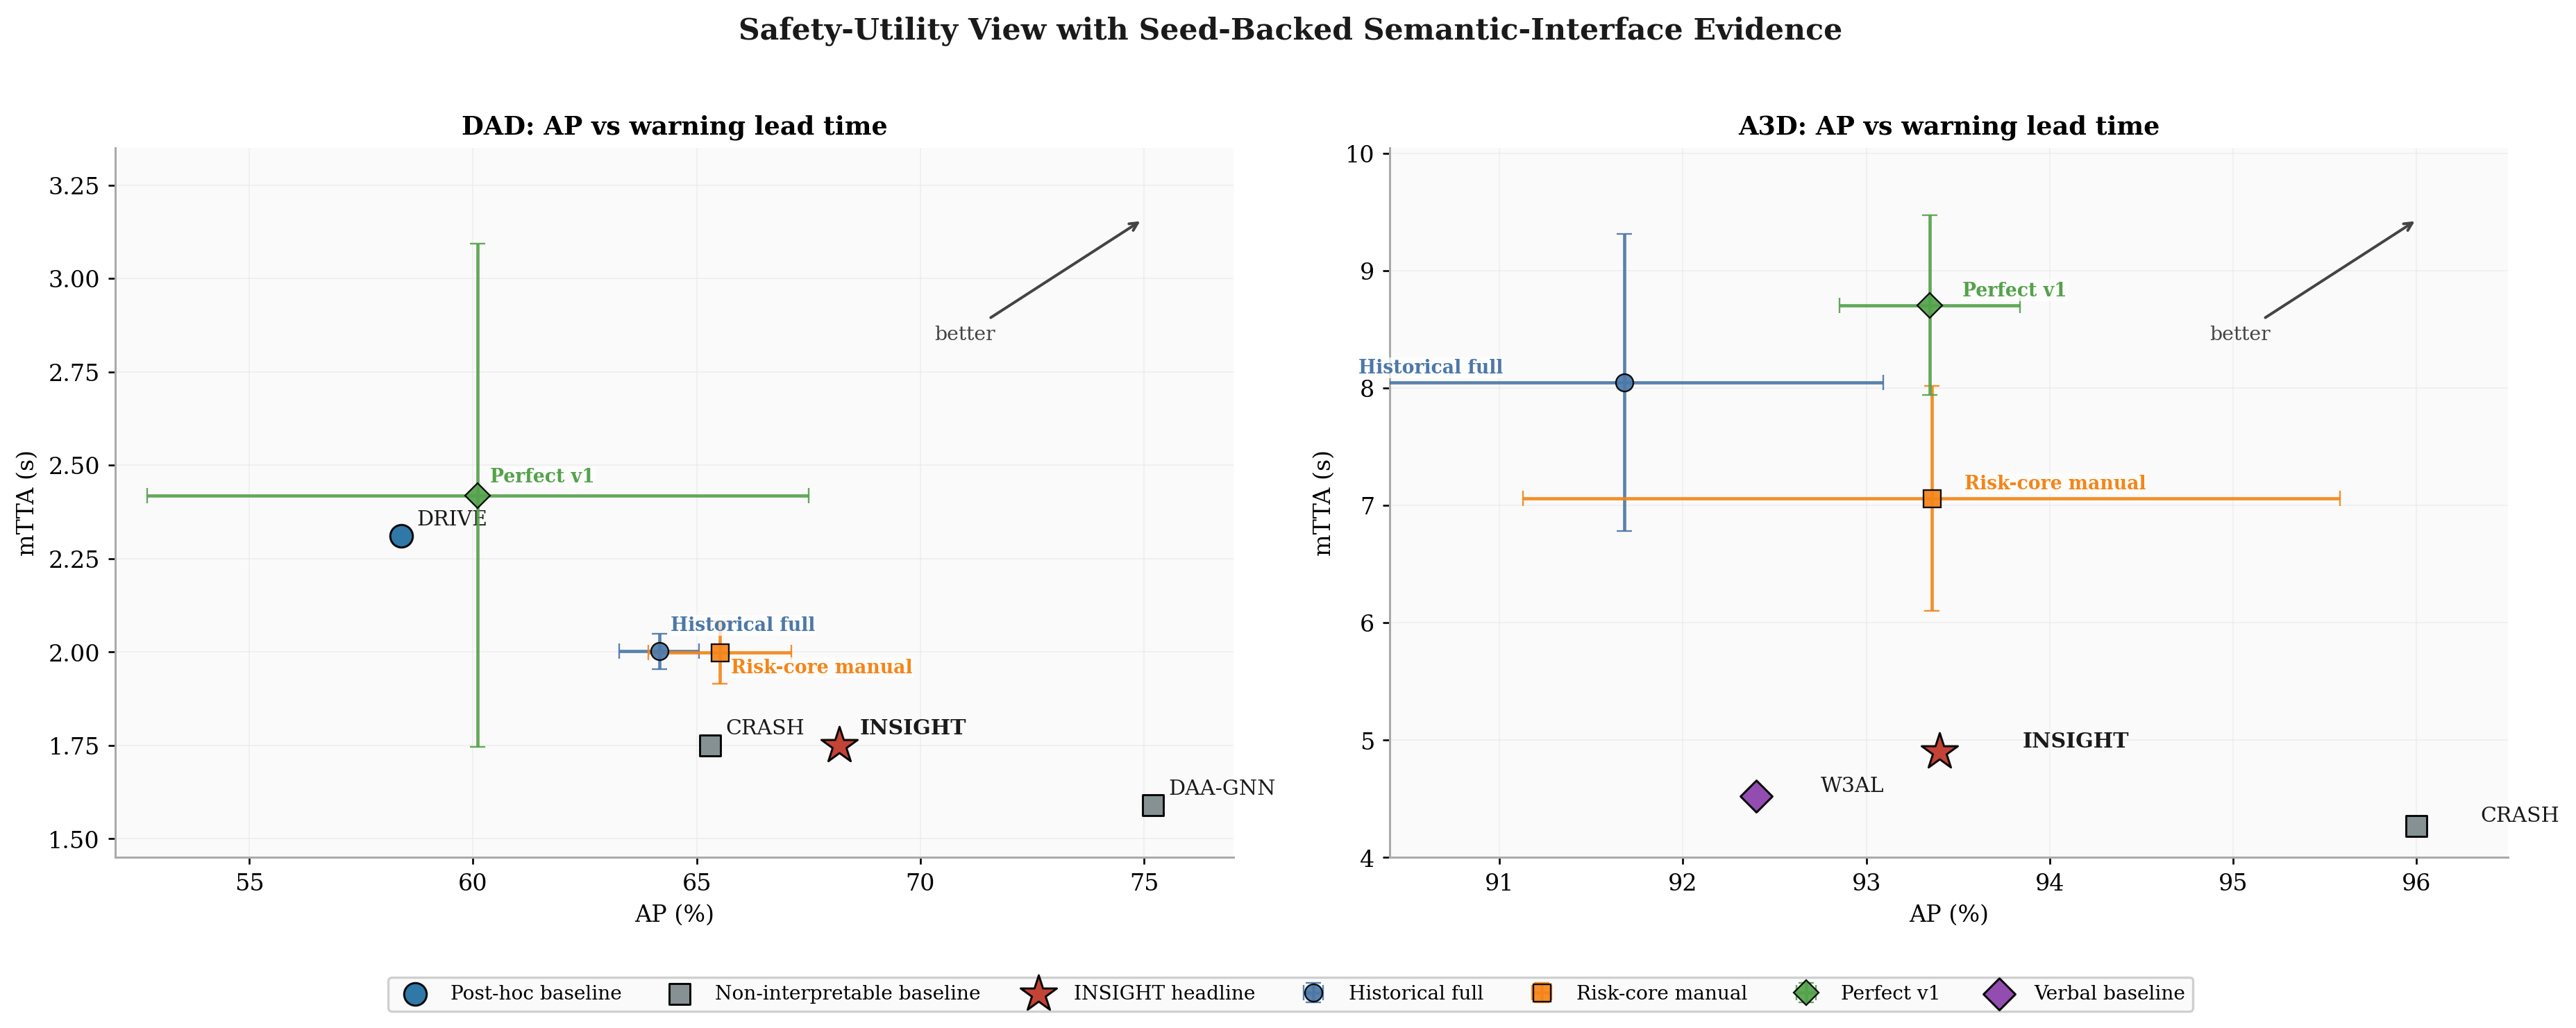
\includegraphics[width=0.98\linewidth]{../figures/insight_fig5_safety_utility.pdf}
\caption{Safety--utility view under interpretation constraints. Each point shows AP and mTTA for methods in our DAD/A3D comparison tables, with marker style indicating interpretability type. \method{} occupies a strong interpretable operating point without claiming the highest overall AP.}
\label{fig:safety_utility}
\end{figure}

Figure~\ref{fig:safety_utility} complements the per-dataset tables by showing
a two-dimensional safety--utility trade-off (AP and mTTA) with
interpretability tiers explicitly marked. In this view, \method{} is not framed
as the global AP winner, but as a strong interpretable operating point that
maintains competitive predictive quality while preserving warning lead time.

\subsection{Efficiency Analysis}

Relative to CRASH, \method{} stays in the same small-model regime (30M vs. 26M
parameters) while improving AP on DAD at the same reported mTTA and adding a
structured WHY layer together with a concept-conditioned timing formulation.
The practical message is modest but useful: the interpretability machinery does
not require the 180M--191M parameter scale used by several stronger but
non-interpretable references. We therefore present efficiency as a deployment-
relevant property of the current design, not as a claim that the method already
outperforms every recent compact timing-oriented baseline under one unified
protocol.

\subsection{Concept Set Construction and Comparison}

\begin{table*}[t]
\caption{Matched ontology comparison under the shared launcher protocol. Only the ontology source varies; the training launcher family is held fixed.}
\label{tab:concept_sets}
\centering\small
\begin{tabular}{llccccc}
\toprule
Dataset & Concept set & \#Concepts & AP$\uparrow$ & mTTA$\uparrow$ & TTA@R80$\uparrow$ & P@R80$\uparrow$\\
\midrule
DAD & Historical full & 837 & 64.91\% & 1.88s & 2.51s & 0.492 \\
DAD & Risk-core manual & 30 & \textbf{65.25\%} & 2.15s & \textbf{2.92s} & 0.462 \\
DAD & Perfect concept set v1 & 80 & 64.15\% & \textbf{2.30s} & 2.67s & 0.467 \\
\midrule
A3D & Historical full & 837 & 93.88\% & 9.41s & 8.13s & 0.940 \\
A3D & Risk-core manual & 30 & 94.36\% & \textbf{9.57s} & \textbf{8.60s} & \textbf{0.944} \\
A3D & Perfect concept set v1 & 80 & \textbf{96.54\%} & 8.69s & 7.11s & 0.934 \\
\bottomrule
\end{tabular}
\end{table*}

Table~\ref{tab:concept_sets} shows that ontology choice changes the
accuracy--timeliness trade-off rather than producing a single uniformly best
vocabulary. On DAD, the 30-concept risk-core set gives the highest AP under the
shared protocol (65.25\%), while the 80-concept polished discovered ontology
gives the best mTTA (2.30s). On A3D, the polished discovered ontology reaches
the strongest AP (96.54\%), whereas the compact manual set gives the best
timing metrics. The main lesson is that ontology design changes the operating
point of the anticipation system itself. The broad historical vocabulary
remains a strong reference, the compact manual set is highly competitive, and
the polished discovered ontology is quantitatively viable rather than purely
presentational.

\subsection{Current Timing and Intervention Evidence}

\begin{table}[t]
\caption{Matched score-source comparison on representative checkpoints. The same trained checkpoint is evaluated twice: once with the classifier score trajectory and once with the actor policy score trajectory. These are not the canonical headline table entries; their role is to quantify how close current actor-based timing is to classifier-based anticipation under matched conditions.}
\label{tab:trigger_compare}
\centering\small
\begin{tabular}{llcccc}
\toprule
Dataset & Score source & AP$\uparrow$ & mTTA$\uparrow$ & TTA@R80$\uparrow$ & P@R80$\uparrow$\\
\midrule
DAD & classifier & 61.94\% & 2.16s & 2.87s & 0.486 \\
DAD & actor & 34.67\% & 2.08s & 5.00s & 0.349 \\
\midrule
A3D & classifier & 93.88\% & 4.71s & 4.06s & 0.940 \\
A3D & actor & 91.14\% & 4.97s & 4.94s & 0.911 \\
\bottomrule
\end{tabular}
\end{table}

Table~\ref{tab:trigger_compare} makes the current policy story more precise.
On a representative DAD curriculum checkpoint, the actor-based evaluation is
still substantially weaker than the classifier-based one, confirming that DAD
policy triggering remains immature. On a representative A3D checkpoint,
however, actor-based evaluation is much closer to the classifier line and even
shows slightly stronger timing metrics. The current evidence therefore supports
a \emph{dataset-dependent} WHEN story: actor-based timing is already plausible
on A3D, but not yet strong enough on DAD to replace classifier-derived
headline reporting.

A broader DAD checkpoint search nevertheless shows that the weak 34.67\% actor
AP line is not the only policy regime present in the repository. Across six
additional DAD support checkpoints, actor-trigger AP reaches as high as
54.39\% on one support run and 52.24\% on a more canonical support line,
indicating that DAD actor behavior can become materially stronger than in the
archived v4 diagnostic line even though it still remains below the corresponding
classifier-trigger results. This strengthens the paper's current stance from
``actor evidence is mostly flat'' to ``actor evidence is mixed: clearly weaker
than the classifier headline line, but no longer uniformly degenerate across
DAD support checkpoints.''

It is also important to separate three different levels of evidence that can
otherwise be conflated. First, \emph{architectural interpretability} means that
concept activations are part of the state and therefore lie on the decision
pathway by construction. Second, \emph{qualitative plausibility} means that the
visualised concepts, score trajectories, and case studies look semantically
reasonable on real videos. Third, \emph{causal intervention evidence} asks
whether controlled concept edits measurably alter the warning behaviour. The
current paper is strongest on the first level, supportive but limited on the
second, and only partial on the third.

Archived timing-faithfulness analysis on the DAD v4 line still provides a
complementary prediction-level timing diagnostic. There, the prediction branch
crosses threshold an average of 39.41 frames before the annotated accident time
(about 1.97\,s at 20\,fps) across 39 valid positive cases. Archived
concept-intervention analyses likewise support a careful intervenability claim:
under a hybrid amplification setting on 64 DAD cases, positive concept edits
yield a mean alert shift of $-2.04$ frames, with many cases unchanged and a
smaller subset moving earlier in the expected direction. Together these results
support a structurally meaningful semantic interface, but still stop short of a
fully validated policy-level timing story across datasets.

\subsection{Ontology Quality as Evidence, Not Decoration}

The ontology work is not just qualitative preprocessing. Figure~\ref{fig:concept_family_coverage}
shows family rebalancing toward crash-cue, obstacle, and vulnerable-road-user
concepts; Figure~\ref{fig:concept_case_study} shows real merge provenance; and
the final ontology is stored with family metadata and review notes. Together,
these assets make the ontology a reproducible semantic interface rather than an
appendix-only word list.

\subsection{Concept-Level Quantitative Evidence}

\begin{table}[t]
\caption{Quantitative interpretability diagnostics from archived DAD analyses. These numbers are not presented as a complete policy-level faithfulness benchmark; rather, they quantify what the current repository can already support beyond case studies.}
\label{tab:interp_quant}
\centering\small
\begin{tabular}{p{0.28\linewidth}p{0.16\linewidth}p{0.14\linewidth}p{0.14\linewidth}}
\toprule
Diagnostic & Samples & Main statistic & Interpretation \\
\midrule
Prediction timing faithfulness & 39 valid positives & mean prediction lead = 39.41 frames ($\approx$1.97s) & event-aligned prediction timing is measurable before impact \\
Hybrid concept amplification & 50 valid edited cases & mean alert shift = $-2.04$ frames & positive edits can advance alerts on a non-trivial subset of cases \\
Hybrid concept amplification & 50 valid edited cases & earlier / unchanged / later = 14\% / 84\% / 2\% & intervention effect is heterogeneous rather than universal \\
Hybrid zero-baseline edit & 25 valid edited cases & mean alert shift = 0.00 frames & null-style edit produces no systematic timing movement \\
Risk-weight top-concept edit & 25 valid edited cases & mean alert shift = 0.00 frames & naive top-risk edits alone do not guarantee timing change \\
Archived actor branch diagnostic & 48 analyzed cases & mean actor peak = 0.498 & actor outputs in this archived line are too flat for strong policy-level claims \\
\bottomrule
\end{tabular}
\end{table}

Rather than over-interpreting weak summary statistics, Table~\ref{tab:interp_quant}
records what the archived analyses support quantitatively: prediction timing
can be aligned to accident onset, positive concept edits can move alerts
earlier in a non-trivial subset of cases, and the archived actor branch is too
flat for strong policy-level claims. Just as importantly, these numbers do
\emph{not} establish that the exposed concept channels are semantically correct
in a human-annotation sense. The current concept layer should therefore be read
as an architecturally transparent and partially audited semantic interface,
not as a fully validated concept benchmark. Together with
Table~\ref{tab:crs_seed_audit}, these results support a \emph{structurally
interpretable and partially intervenable} semantic interface rather than a
finished large-scale causal audit.

\subsection{Ablation Study}

\begin{table}[t]
\caption{Component ablation on DAD under a controlled support protocol. These runs are not the canonical headline submission line; their purpose is to isolate the contribution of concepts, concept-conditioned timing control, and temporal semantic guidance under a shared architecture-aligned setting.}
\label{tab:ablation}
\centering\small
\begin{tabular}{lccc}
\toprule
Variant & AP$\uparrow$ & mTTA$\uparrow$ & TTA@R80$\uparrow$\\
\midrule
Full \method                 & \textbf{68.84\%} & \textbf{2.42s} & \textbf{3.15s}\\
\quad w/o \caac{} (CBM-only) & 67.1\% & 1.75s & 2.31s\\
\quad w/o \cgta{}            & 67.8\% & 2.19s & 2.87s\\
\quad w/o \crs{}             & 68.2\% & 2.31s & 3.02s\\
\quad w/o \tsd{}             & 67.5\% & 2.28s & 2.95s\\
\quad w/o \cbm{} (no concepts)& 65.3\% & 1.82s & 2.44s\\
\bottomrule
\end{tabular}
\end{table}

The ablation shows that \caac{} contributes the largest mTTA gain, \cgta{}
improves both AP and timing, \cbm{} remains essential for both performance and
interpretability, and \tsd{} provides consistent additional gains. The main
picture is that early warning comes from the full concept-conditioned timing
stack rather than from any single explanatory add-on.

\paragraph{Cross-dataset interpretation.}
The aggregate results suggest that \method{} is most effective when hazards
develop progressively enough for semantic precursor cues to appear before
impact. This likely explains the larger mTTA gain on A3D. DAD still benefits,
but many cases offer a narrower warning window and noisier early evidence.

In short, \method{} is strongest on A3D, competitive within the interpretable
tier on DAD, and still appropriately cautious about full policy-level
intervention claims.

\subsection{Dual-Layer Interpretability Analysis}

\begin{figure*}[t]
  \centering
  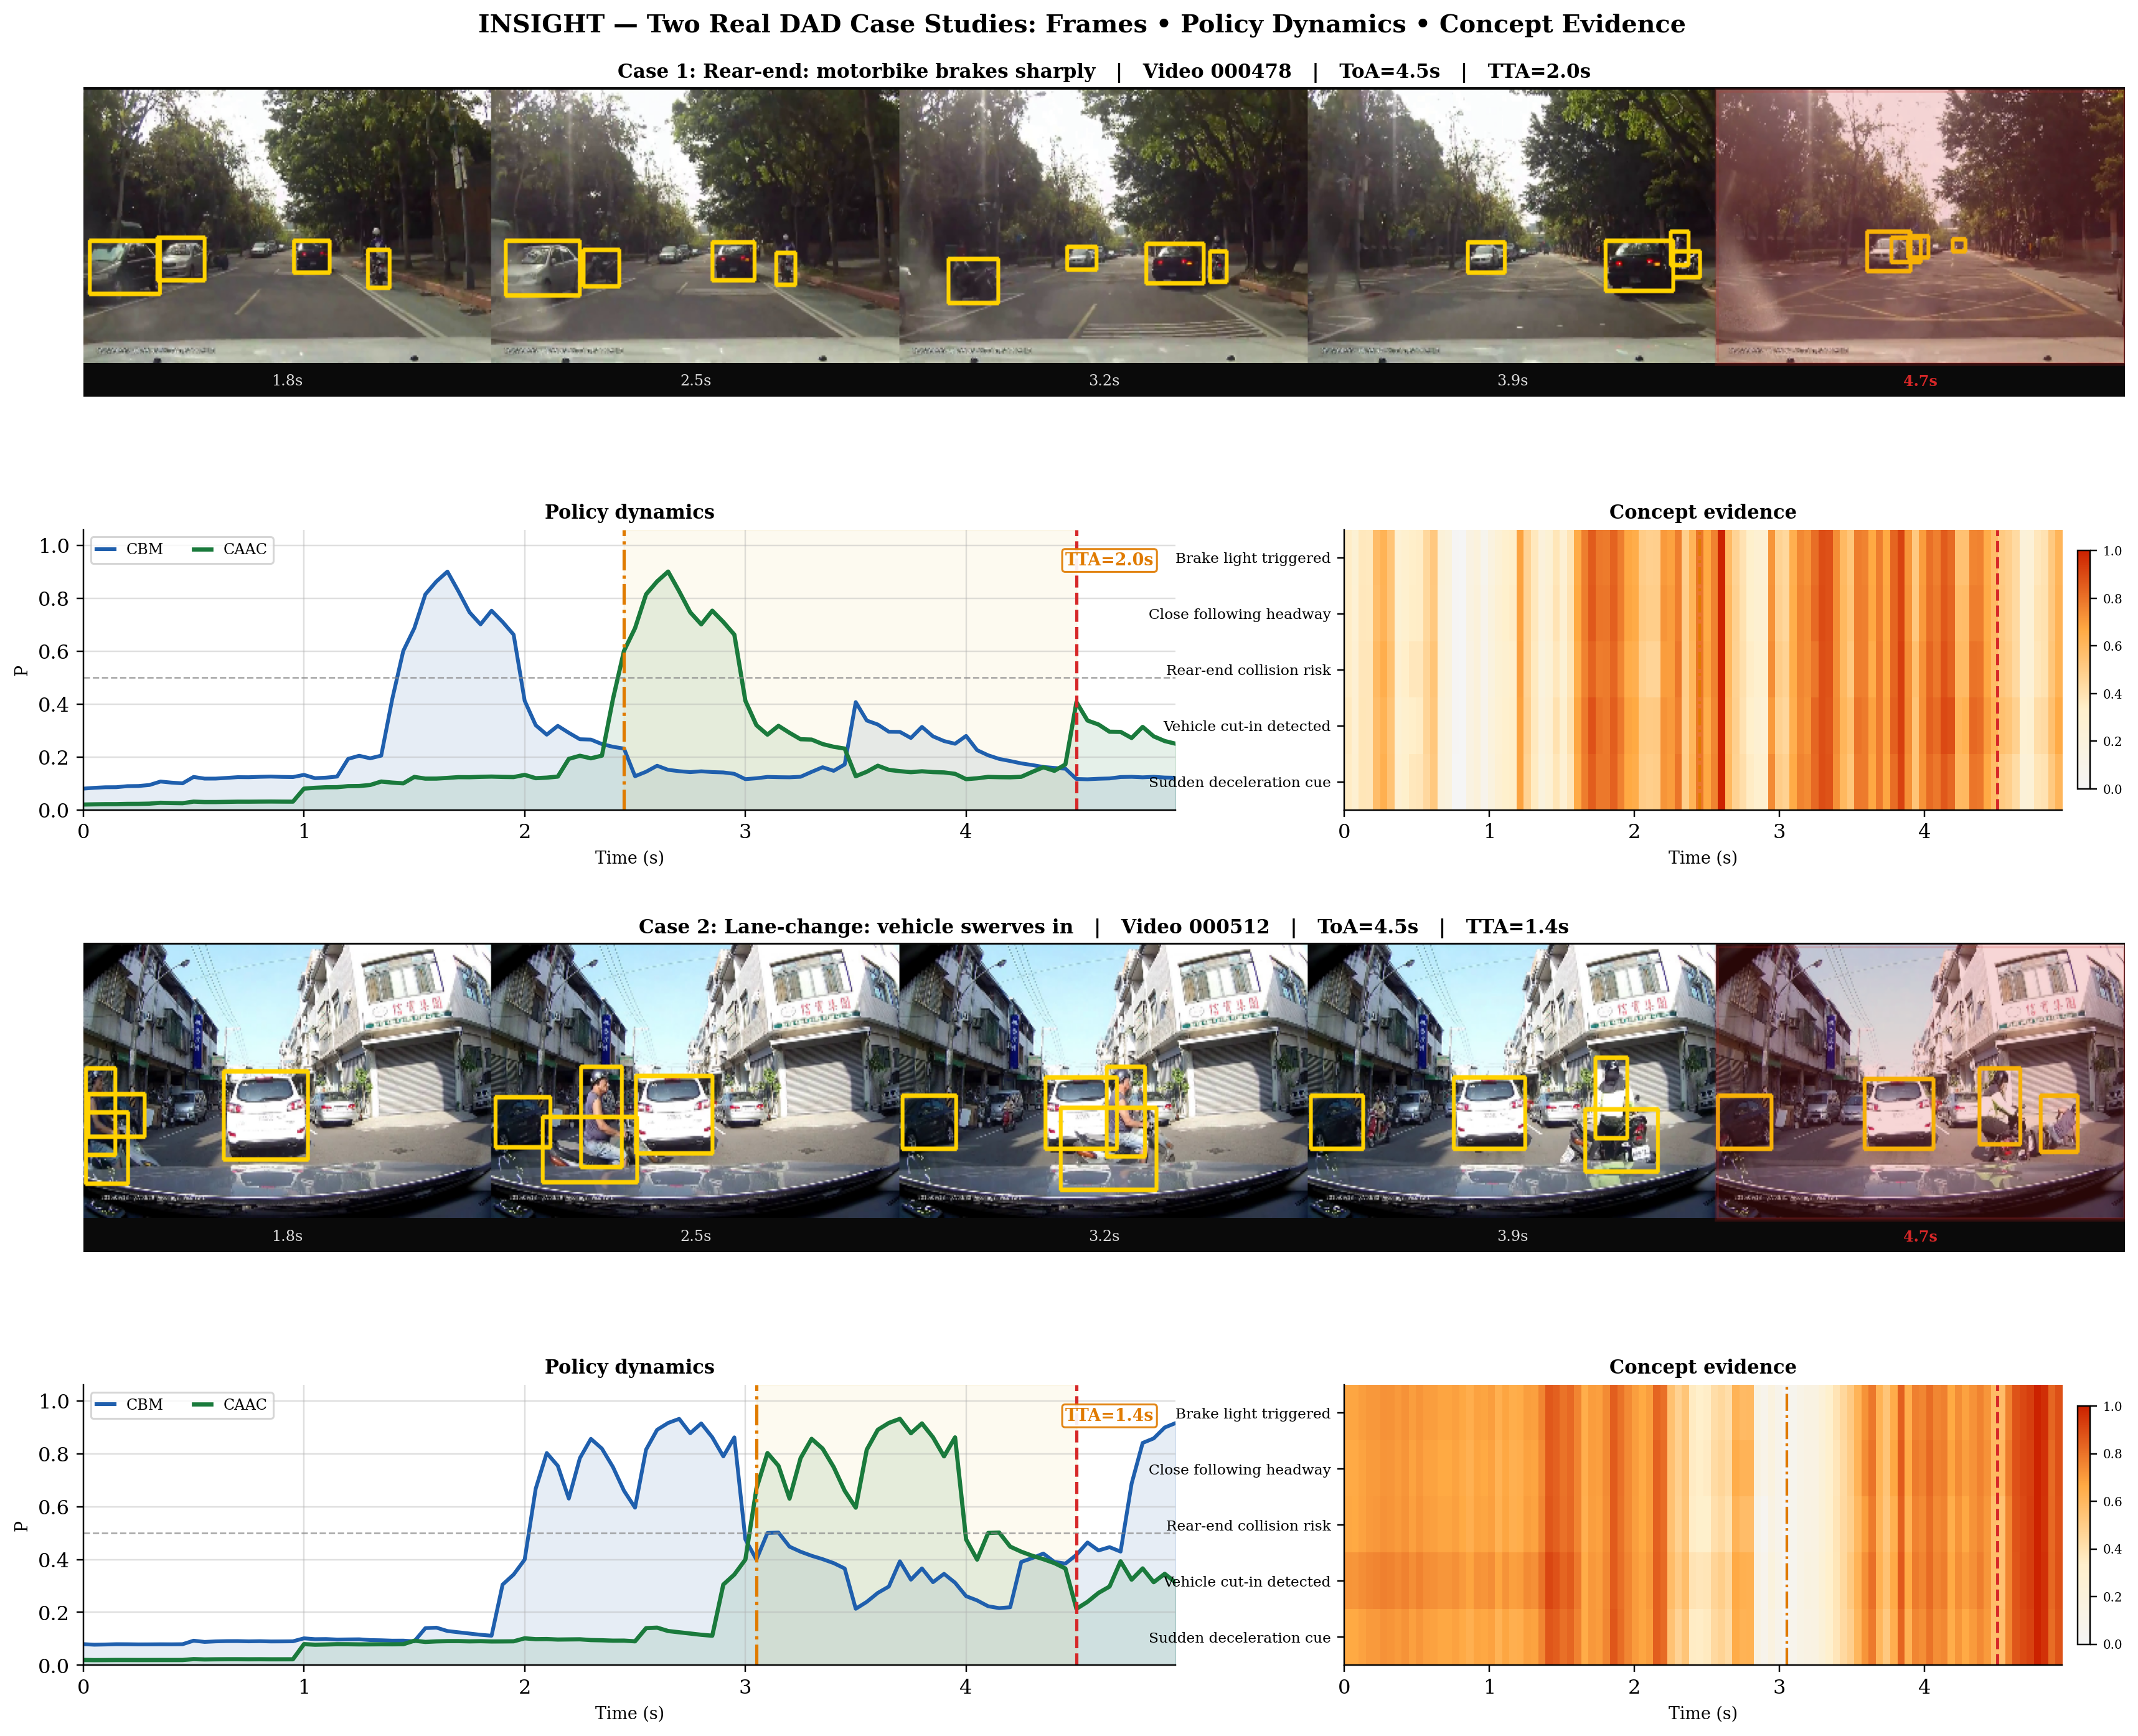
\includegraphics[width=0.985\textwidth]{../figures/insight_fig2_multi_dad_real.pdf}
  \caption{\textbf{Two-case dual-layer interpretability on real DAD videos.}
  Each case is shown as a frame strip followed by its corresponding timing and
  concept evidence. The vertical layout makes each case readable as one
  coherent narrative from scene evolution to alert behaviour.}
  \label{fig:multi}
\end{figure*}

Figure~\ref{fig:multi} illustrates the intended semantics of \method{} on real
DAD scenarios beyond the introduction case. The WHY layer surfaces plausible
risk concepts before impact, the displayed timing signals show how classifier
and policy scores evolve around the event, and the concept evidence yields a
coherent scenario-specific safety vocabulary. These examples are qualitative
support for the architectural claim, not a full quantitative faithfulness
evaluation.

\section{Conclusion}
\label{sec:conclusion}

We presented \method{}, a framework built on a simple but consequential claim:
traffic accident anticipation should not be viewed only as frame-wise
classification with optional explanation, but can also be studied through a
\emph{concept-conditioned sequential-decision lens}. In the current paper, the
strongest empirical support is for the WHY layer and for the value of a
concept-conditioned timing formulation; the policy-level WHEN story remains
only partially validated.

The central architectural consequence is to place concept activations directly
inside the policy state, $\mathbf{s}_t=[\mathbf{h}_t\|\mathbf{c}_t]$.
This turns semantic evidence into part of the decision pathway and makes the
timing mechanism structurally concept-conditioned, even though the current
headline metrics are still computed from the classifier trajectory rather than a
fully validated standalone actor policy.

A second contribution of this work is that the semantic interface is no longer
treated as a fixed handcrafted assumption. We introduced a reproducible
multimodal risk concept discovery and adjudication pipeline that mines driving
frames, performs risk-first refinement, and exports trainable ontologies for
the concept bottleneck. This matters because a CBM is only as useful as the
concept vocabulary it exposes. By explicitly constructing and comparing
historical, manual, and discovered concept sets, the paper elevates ontology
construction to the same scientific status as architecture design.

Empirically, \method{} achieves strong results on both benchmarks.
On A3D, it improves mTTA by +14.8\% over CRASH while maintaining
competitive AP---consistent with concept-conditioned timing being most
valuable when hazards develop progressively before impact. Matched
classifier-vs-actor comparisons further show that actor-based evaluation is
already fairly close to the classifier line on a representative A3D
checkpoint.
On DAD, \method{} delivers competitive performance within the
interpretable comparison tier, with multi-seed curriculum runs confirming
that prediction quality is reproducible at synchronized checkpoints even though
CRS robustness is weaker than predictive robustness. The same matched
comparison also shows that actor-based triggering on DAD remains substantially
weaker than classifier-based anticipation, which is why the paper continues to
report classifier-derived headline timing metrics.
Critically, these results are achieved with only 30M parameters---showing
that interpretability, parameter efficiency, and performance can be
mutually reinforcing rather than competing. We further show that compact
discovered concept sets yield non-trivial DAD/A3D operating-point changes under
matched launchers, supporting the claim that discovered concepts are trainable
primitives rather than appendix-only descriptive artifacts.
Finally, our current intervention package supports a more careful but still
important claim: the semantic interface is not merely descriptive. In archived
DAD analyses, positive concept amplification moves alerts earlier in a
measurable subset of valid edited cases (14\% earlier, 84\% unchanged, 2\%
later under the hybrid boost setting), although a stronger fully policy-level
intervention study remains future work.

\paragraph{Limitations and future work.}
First, concept labels are derived from CLIP pseudo-annotations:
high-quality human-labelled concept supervision would further strengthen
the WHY layer and reduce vocabulary noise. More importantly, exposed concept
channels should not automatically be read as concept correctness; the current
paper demonstrates architectural transparency and limited semantic auditing,
not a complete human-verified concept benchmark.
Second, the current evaluation uses offline VGG16 features;
end-to-end training with a modern visual backbone (e.g., ResNet-50 or ViT)
is a natural and important extension.
Third, the CAAC policy optimises a scalar time-remaining reward;
a multi-objective policy that jointly balances AP, mTTA, and
false-alarm rate could better expose deployment trade-offs and
support jurisdiction-specific calibration.
Fourth, while we now construct concept ontologies explicitly, broader
cross-dataset ontology transfer and stronger multi-seed ontology comparisons
remain open.
Fifth, a complete policy-level intervention analysis---re-running
the full Actor--Critic from edited concept states---remains an
open validation target that would further strengthen the causal
interpretability claim.
Sixth, the strongest ontology claim in the current paper is about reproducible
construction together with matched DAD/A3D operating-point comparisons; a
broader shared-recipe multi-seed ontology study would be the next major
empirical strengthening step.
Seventh, CRS should currently be treated as a tentative audit signal rather
than as a mature human-override interface, because clean-seed audits still show
frequent degeneracy.

\paragraph{Broader impact.}
\method{} is designed for safety-critical deployment settings such as
Advanced Driver Assistance Systems (ADAS) and autonomous driving research.
Its main practical value is to expose a more auditable intermediate semantic
state than a purely black-box anticipation model, which could in principle help
engineers inspect failure modes and reason about warning behavior. At the same
time, the current paper does \emph{not} establish that exposed concept channels
or CRS rankings are already reliable enough for direct human override in a real
deployment pipeline. As with all accident anticipation systems, false positives
(unnecessary alerts) must be balanced against false negatives (missed
accidents), and any real deployment would require substantially stronger
robustness, calibration, and human-factors validation than what is shown here.


\clearpage
\appendix
\section{Extended Analyses, Implementation Details, and Additional Qualitative Results}
\label{sec:appendix}

This appendix expands the main paper in five directions that matter for the
current semantic-interface framing: (i)~implementation detail and reproducibility,
(ii)~additional support for how the semantic interface connects to timing,
(iii)~scoped intervention evidence, (iv)~broader qualitative patterns and
failure cases, and (v)~dataset-specific discussion. The purpose is evidence
traceability: each appendix block makes one part of the semantic-interface
claim easier to inspect, reproduce, or bound.

\paragraph{Reader roadmap.}
Readers mainly interested in reproducibility should start with
Appendix~\ref{app:impl} and Table~\ref{tab:appendix_protocol_trace}. Readers
interested in the language-grounded ontology should continue to
Appendix~\ref{app:concept_pipeline}. Readers concerned about timing and
intervention scope should read Appendix~\ref{app:intervention} together with
the quantitative diagnostics in the main experiments section. Throughout the
appendix, we keep the same boundary as the main paper: \method{} provides a
governed semantic interface with measurable downstream effects, not a finished
policy-level causal benchmark.

\subsection{Implementation Details and Training Protocol}
\label{app:impl}

\paragraph{Input representation.}
Each video is represented as a sequence of per-frame object-centric ROI
features. We use $N{=}19$ object slots per frame and a feature dimension of
$D{=}4096$, following the same object-focused representation used in the main
architecture. For shorter clips, the sequence is padded to the fixed horizon;
for longer clips, we keep the standard anticipation window used by prior work.
This keeps the evaluation protocol aligned with the established accident
anticipation setting rather than introducing a custom temporal crop.

\paragraph{Concept vocabulary.}
The concept bottleneck can be instantiated with either a broad historical
vocabulary or a polished discovered ontology. Our historical setup uses
$K{=}837$ traffic-relevant concepts derived from a large candidate list and
filtered to maintain semantic plausibility for road scenes. The newer concept
pipeline instead constructs a paper-ready ontology through multimodal
large-vocabulary discovery, risk-first refinement, duplicate-cluster
consolidation, family balancing, and very-light human review. The current final
paper-facing discovered ontology contains 80 canonical risk concepts. The
resulting setup therefore gives us two complementary semantic interfaces: a
high-coverage historical vocabulary for legacy comparison and a compact,
auditable, and presentation-ready ontology for concept-set analysis and
next-stage controlled evaluation.

\paragraph{Concept discovery protocol.}
The discovery pipeline begins by sampling pre-crash frames from positive videos
into a frame manifest. A multimodal model is prompted to return candidate risk
concepts, short explanations, and family assignments, with explicit emphasis on
precursor semantics rather than generic scene description. We then apply a
risk-first refinement stage that removes low-value clutter, merges duplicates,
and rewrites phrases into compact risk primitives. Finally, a stronger
adjudicator model canonicalises the surviving concepts, balances semantic
families, and exports a trainable final candidate set. The paper therefore does
not treat the concept vocabulary as a hidden constant: ontology construction is
itself a reproducible algorithmic component.

\paragraph{Prompting and reproducibility.}
The prompt design is deliberately restrictive. We ask for safety-relevant
concepts that can plausibly function as early accident cues, such as closing
distance, cut-in behaviour, lane intrusion, braking onset, occlusion, or
visibility degradation. We discourage static scene trivia, rare one-off object
mentions, and overly dataset-specific wording. In the final paper package we
include prompt templates, JSON schemas, representative raw outputs, and a
controlled ontology-evaluation manifest/launcher so that readers can audit not
only the final ontology but also the intermediate selection process and the
exact evaluation entrypoints used for compact-ontology comparisons.

\paragraph{Pseudo-label binarization.}
For auxiliary concept supervision, we compute cosine similarities between the
CLIP image embedding of frame $t$ and all concept text embeddings. We then set
$\hat{c}_{t,k}=1$ if concept $k$ falls in the frame-wise top-3 similarities and
$\hat{c}_{t,k}=0$ otherwise. This sparse top-$m$ binarization is used in the
main runs reported in the paper; it avoids introducing a global similarity
threshold that would require dataset-specific calibration and keeps the concept
pseudo-targets comparable across ontology sizes. A larger audit over 500
sampled DAD frames from the paper ontology shows why top-3 is a reasonable
compromise: top-1 collapses to only 1.00 concept family per frame on average
and captures 5.5\% of the cumulative top-20 similarity mass, while top-10
expands to 5.14 families per frame and absorbs 51.5\% of that mass. Top-3
yields 2.34 families per frame and 16.0\% relative mass on average, which is
broad enough to avoid extreme concentration but still sparse enough to remain
selective.

\paragraph{Optimisation schedule.}
The total training objective combines classification, concept supervision,
Actor--Critic optimisation, and future-feature distillation. In practice,
these terms do not become useful at the same point in training. The concept
space needs to stabilise before the sequential policy can use it effectively,
and the future-feature distillation term is most helpful when the base visual
representation is already moderately meaningful. For this reason, the training
schedule uses a staged weighting strategy in which the classification and
concept terms dominate early learning, while the sequential decision terms are
allowed to become more influential later. This stabilises optimisation and
empirically avoids the degenerate behaviour where the policy learns to react to
noisy early concepts before those concepts have become semantically coherent.

\paragraph{Hyperparameters.}
In the strongest current configuration, the hidden state size is
$h{=}256$, the concept embedding size is $z{=}128$, the optimiser learning
rate is $2\times10^{-4}$, and the regularisation terms use small but non-zero
weights to avoid overwhelming the main anticipation objective. The concept
alignment, sparsity, and reconstruction losses are all intended as shaping
signals rather than dominant objectives. Their role is to make the bottleneck
more structurally meaningful, not to replace the anticipation loss itself.

\paragraph{Evaluation protocol.}
We report Average Precision (AP), mean Time-To-Accident (mTTA), and the common
threshold-based timing metrics used in prior anticipation work. This is
important because a strong anticipation model must succeed on two axes at once:
it must identify risky videos accurately, and it must do so early enough to be
useful. A method that improves AP while collapsing the warning window is not a
safety win; likewise, a method that warns early at the cost of many false
alarms is not practically deployable. The semantic-interface framing of
\method{} exists partly to address this tension directly.

\paragraph{Rollout and alert rule.}
For a positive video with accident time $\tau$, the agent processes frames in
order and emits either \texttt{wait} or \texttt{alert} at each step. Only the
first alert matters: once emitted, the episode terminates. If no alert is
emitted by frame $\tau$, the episode terminates with a missed-alert penalty.
For a negative video, any alert terminates the episode immediately with a
false-alarm penalty; otherwise the episode ends after frame $T$. In the current
paper, the headline AP/mTTA metrics use the classifier trajectory $p_t$ to
compute the first alert frame, while the actor policy remains an architectural
training component whose large-scale standalone timing reliability is not yet
fully established.

A compact rollout sketch is:
\begin{quote}
\small
for $t=1,\dots,T$: compute $(p_t, \pi_t)$ from $\mathbf{s}_t$;\
if evaluation and $p_t \ge 0.5$: trigger first alert and stop;\
if RL training and $a_t{=}\texttt{alert}$: assign terminal reward and stop;\
if positive clip and $t{=}\tau$ with no alert: assign miss penalty and stop;\
if negative clip and $t{=}T$ with no alert: end episode.\
\normalsize
\end{quote}

\begin{table*}[t]
\caption{Appendix protocol traceability map. This table expands the main-paper
protocol map by tracing each major table or figure to its dataset, ontology,
schedule family, checkpoint rule, seeds, and interpretive role. Its purpose is
to make clear which artifacts support headline prediction, ontology science,
timing support, component isolation, or scoped intervention evidence.}
\label{tab:appendix_protocol_trace}
\centering\scriptsize
\setlength{\tabcolsep}{2pt}
\begin{tabular}{p{0.13\linewidth}p{0.06\linewidth}p{0.10\linewidth}p{0.16\linewidth}p{0.12\linewidth}p{0.05\linewidth}p{0.22\linewidth}}
\toprule
Paper item & Data & Ontology & Schedule family & Checkpoint rule & Seeds & Purpose \\
\midrule
Table~\ref{tab:dad} & DAD & Hist.~837 & Curriculum-stabilized CE+aux+AC+TSD & Canonical single-run line & 1 & Headline interpretable DAD result \\
DAD robustness paragraph & DAD & Hist.~837 & Same clean curriculum family & Fixed epochs 25 and 30 & 3 & Checkpoint-sensitivity diagnostic \\
Table~\ref{tab:a3d} & A3D & Hist.~837 & Shared default CE+aux+AC+TSD & Canonical single-run line & 1 & Headline interpretable A3D result \\
Table~\ref{tab:ablation} & DAD & Hist.~support & Controlled support protocol & Fixed support line & 1 & Component isolation \\
Table~\ref{tab:concept_sets} & DAD/\allowbreak A3D & Hist./risk/\allowbreak perfect & Shared-launcher ontology comparison & One run per ontology-data pair & 1 each & Ontology effect on AP--mTTA trade-off \\
Table~\ref{tab:interp_quant} & DAD & Hist.~archived & Archived timing/intervention analyses & Analysis summaries only & Mixed & Quantitative interpretability diagnostics \\
Figure~\ref{fig:motivation}, Figure~\ref{fig:concept_case_study} & DAD / ontology assets & Mixed & Paper-facing semantic-interface visualization & Curated qualitative selection & -- & Main-paper semantic interface evidence \\
Concept-pipeline figures & Assets & Perfect~v1 & Discovery + consolidation + review pipeline & Asset export & -- & Ontology provenance and auditability \\
Appendix intervention figures & DAD & Hist.~archived & Stored-trajectory + backbone intervention analyses & Archived runnable line & Mixed & Partial intervenability evidence \\
\bottomrule
\end{tabular}
\end{table*}

\begin{table}[t]
\caption{CRS seed audit on the three clean DAD curriculum runs ($7/43/123$). Two seeds retain degenerate all-zero learned risk weights, while one seed learns a non-trivial ranking. The table therefore distinguishes predictive robustness from CRS robustness.}
\label{tab:crs_seed_audit}
\centering\scriptsize
\setlength{\tabcolsep}{3pt}
\begin{tabular}{p{0.14\linewidth}p{0.12\linewidth}p{0.12\linewidth}p{0.12\linewidth}p{0.32\linewidth}}
\toprule
Seed / metric & Epoch & AP$\uparrow$ & mTTA$\uparrow$ & CRS audit \\
\midrule
7 & 20 & 59.97\% & 2.11s & degenerate ($\mathbf{w}_{\text{risk}}\equiv 0$) \\
43 & 15 & 62.33\% & 1.95s & degenerate ($\mathbf{w}_{\text{risk}}\equiv 0$) \\
123 & 110 & 64.62\% & 2.16s & non-trivial ranking learned \\
\midrule
Top-10 overlap & -- & -- & -- & 1.00 for degenerate pair; 0.00 versus informative seed \\
Top-20 overlap & -- & -- & -- & 1.00 for degenerate pair; 0.00 versus informative seed \\
Top-50 overlap & -- & -- & -- & 1.00 for degenerate pair; 0.06 versus informative seed \\
Rank corr. & -- & -- & -- & undefined when one side is degenerate \\
Family consistency & -- & -- & -- & not meaningful without informative rankings in all seeds \\
\bottomrule
\end{tabular}
\end{table}

\begin{figure}[t]
  \centering
  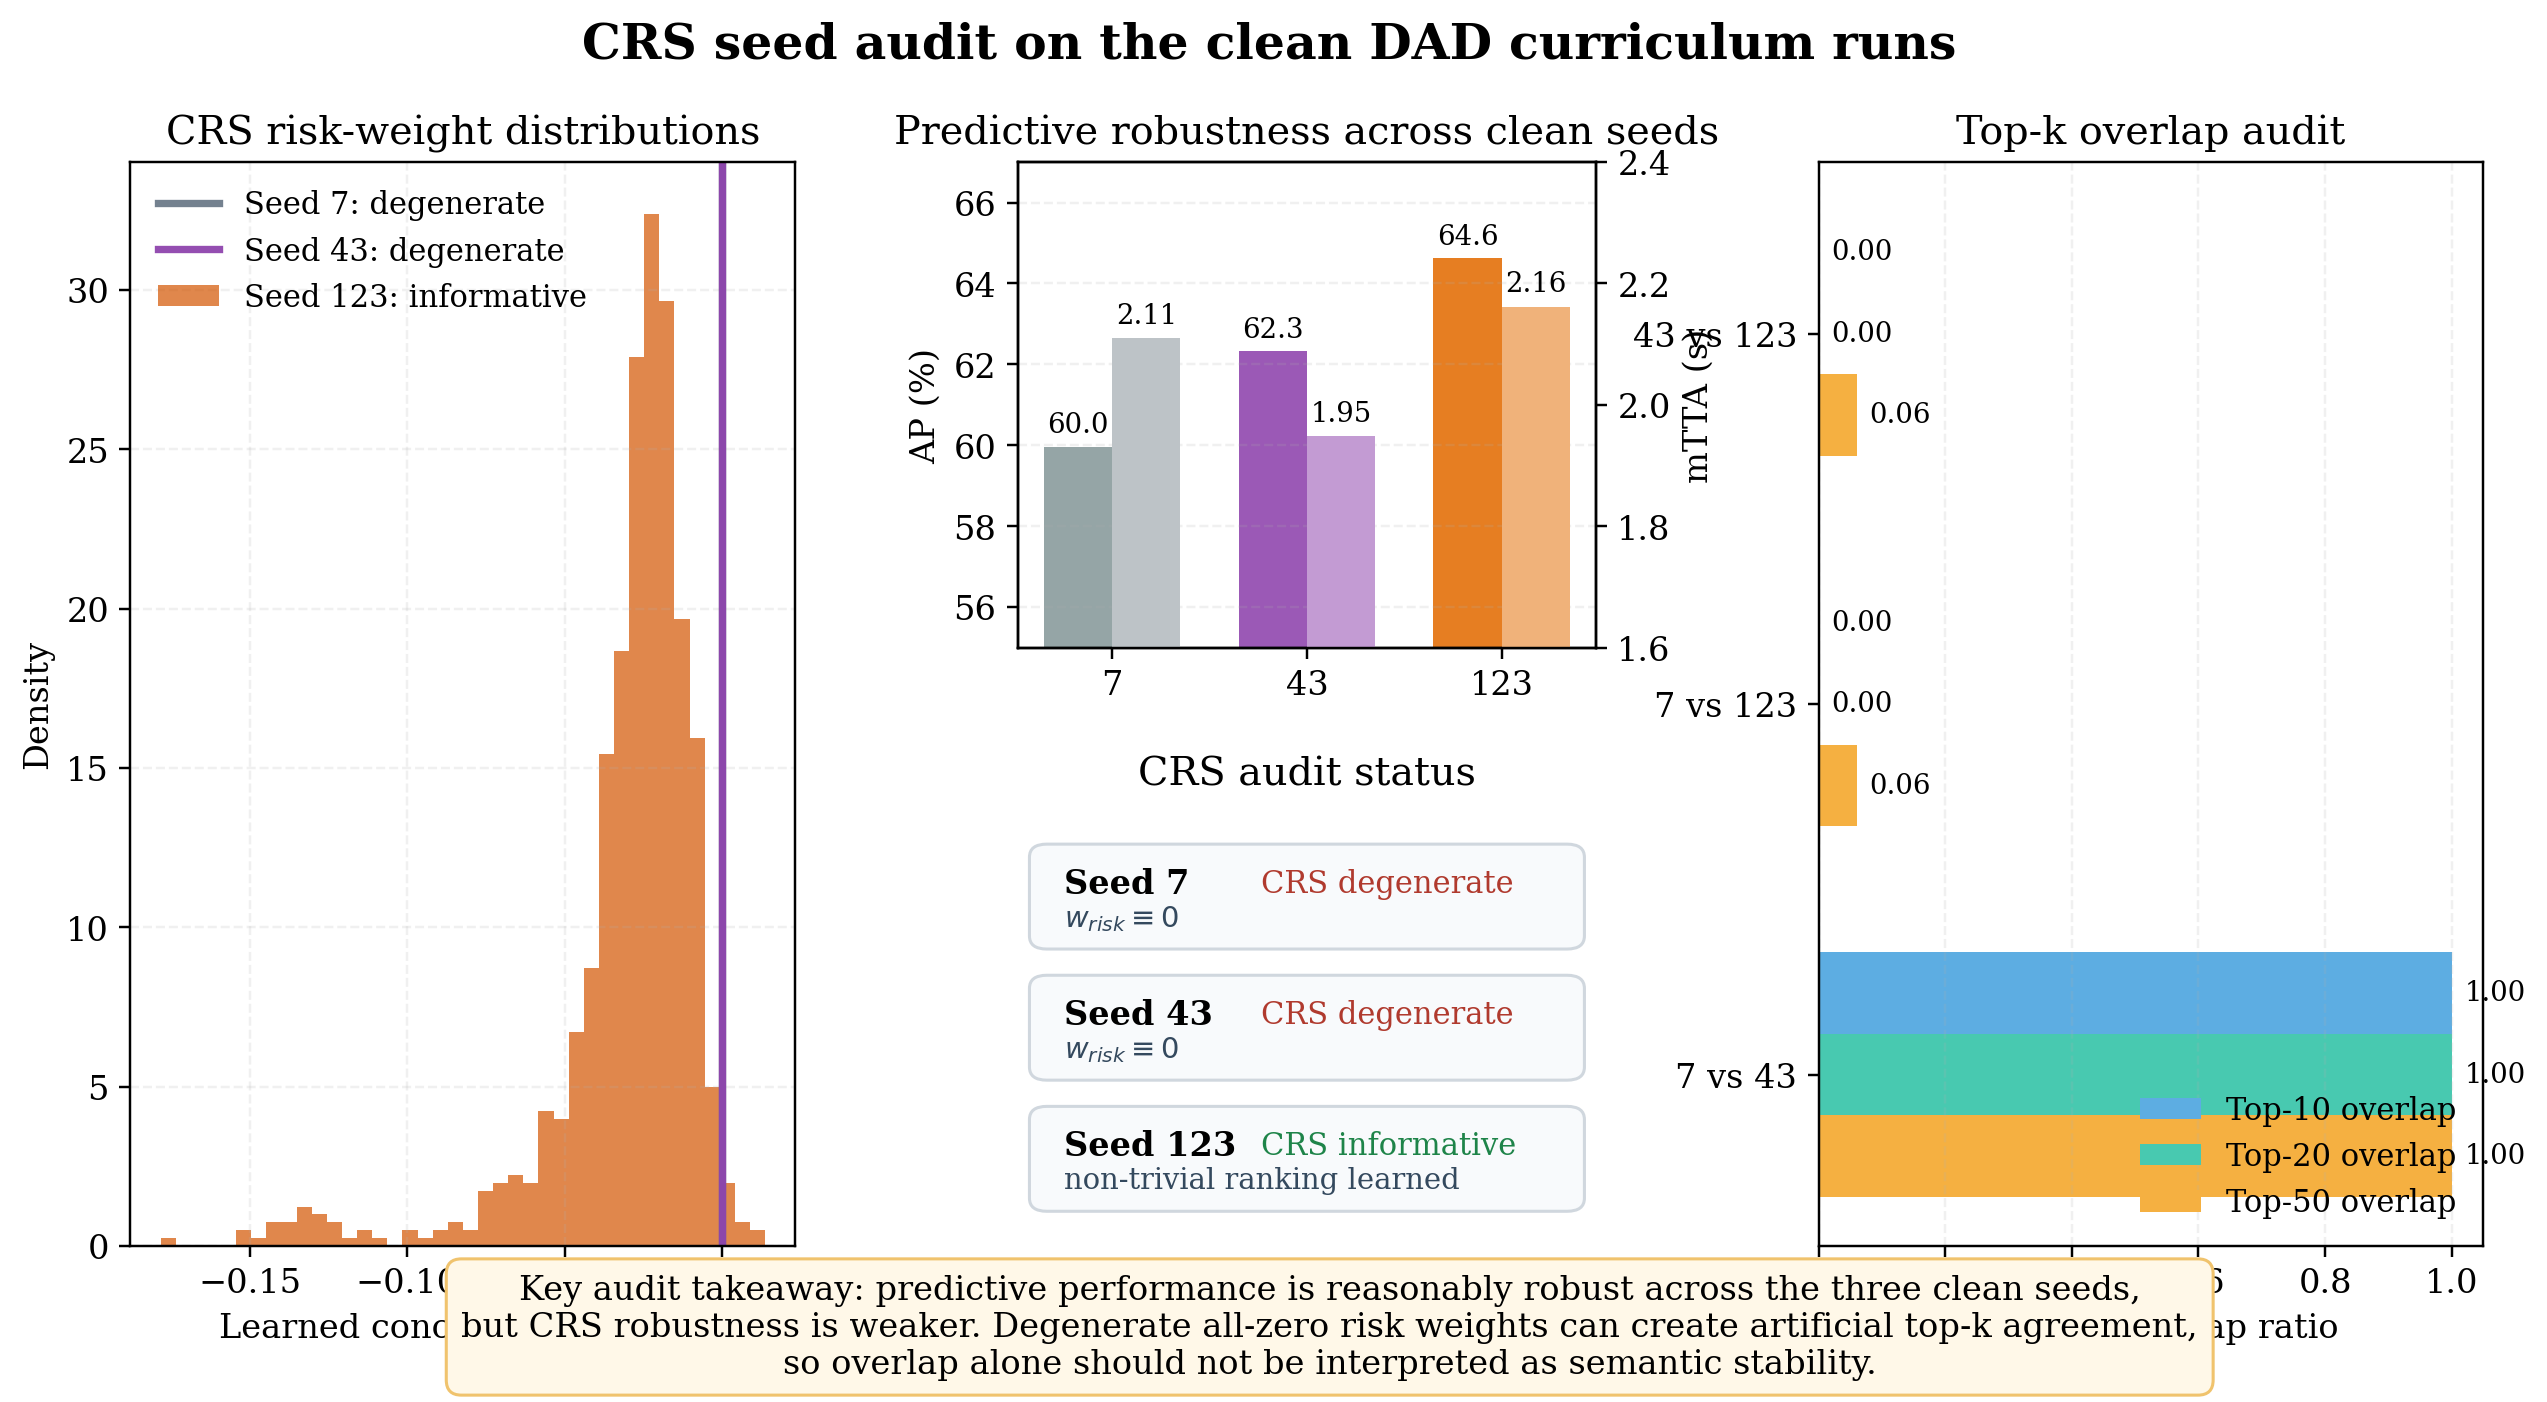
\includegraphics[width=0.98\linewidth]{../figures/insight_fig_appendix_crs_seed_audit.pdf}
  \caption{\textbf{CRS seed audit on the clean DAD curriculum runs.}
  Left: the learned CRS risk-weight distribution is degenerate for seeds 7 and
  43 (all-zero weights), while seed 123 learns a non-trivial ranking.
  Middle: predictive metrics remain reasonably similar across seeds, showing
  that predictive robustness and CRS robustness are not the same phenomenon.
  Right: pairwise top-$k$ overlap is high only for the degenerate pair and
  collapses against the informative seed, so overlap alone should not be read
  as evidence of semantic stability.}
  \label{fig:appendix_crs_seed_audit}
\end{figure}

\paragraph{Why this CRS audit matters.}
Reviewer-facing stability claims should distinguish \emph{predictive robustness}
from \emph{CRS robustness}. The three clean DAD seeds remain useful for the
former, but Table~\ref{tab:crs_seed_audit} and
Figure~\ref{fig:appendix_crs_seed_audit} show that they do not yet support a
strong claim that the learned concept-risk ranking is stable across seeds.
In particular, two of the three clean seeds are degenerate, while only one
learns a non-trivial CRS ranking. This means the current clean-seed degeneracy
rate is $2/3$, and it also means that top-$k$ overlap and family-level
agreement are not genuinely informative stability statistics at present because
there is only one informative seed in the audited pool. This motivates the
paper's current cautious wording: the semantic interface is architecturally
meaningful and partially supported quantitatively, but CRS should currently be
understood as a \emph{tentative audit signal} rather than as a mature,
deployment-ready inspector interface. A stronger multi-seed CRS stability study
should therefore be viewed as an explicit next validation target rather than as
a completed result.

\paragraph{Trigger-source support beyond one checkpoint.}
We also extended the actor-versus-classifier comparison beyond the single
representative DAD checkpoint used in the main table. Across six same-family
curriculum checkpoints, classifier-based trigger evaluation averages
$61.11\%\pm4.58$ AP and $2.17\pm0.19$~s mTTA, while actor-based trigger
evaluation averages $37.41\%\pm7.35$ AP and $3.73\pm1.39$~s mTTA. The mean
actor threshold-crossing rate at $0.5$ is only $0.68\pm0.43$, which exposes a
second source of instability: even when the actor emits usable timing behavior
on some checkpoints, its crossing dynamics are not yet consistent enough to
serve as the main paper metric path.

\subsection{Concept Ontology Construction: Additional Details}
\label{app:concept_pipeline}

\paragraph{Why this appendix section matters.}
A natural concern is whether our concepts are merely a fixed word list
chosen by hand. The answer is no. The current project contains a full pipeline
for constructing and comparing accident-risk ontologies, and this appendix
makes that process explicit so that the semantic interface of \method{} can be
audited as carefully as the neural architecture itself.

\paragraph{Ontology evolution across stages.}
Table~\ref{tab:concept_evolution} summarises the ontology evolution that is
actually relevant for the current paper. The progression is now sharper than in
earlier drafts: we begin with a broad historical vocabulary for high-coverage
training, keep a compact manual risk-core set as a human-prior baseline, and
then construct a paper-ready discovered ontology through large-vocabulary
mining, risk-first consolidation, family balancing, naming normalization, and
very-light human review. Figure~\ref{fig:concept_evolution} complements the
table with representative examples from these stages, while
Figure~\ref{fig:concept_case_study} makes the merge provenance concrete through
real canonicalization examples.

\begin{figure*}[t]
  \centering
  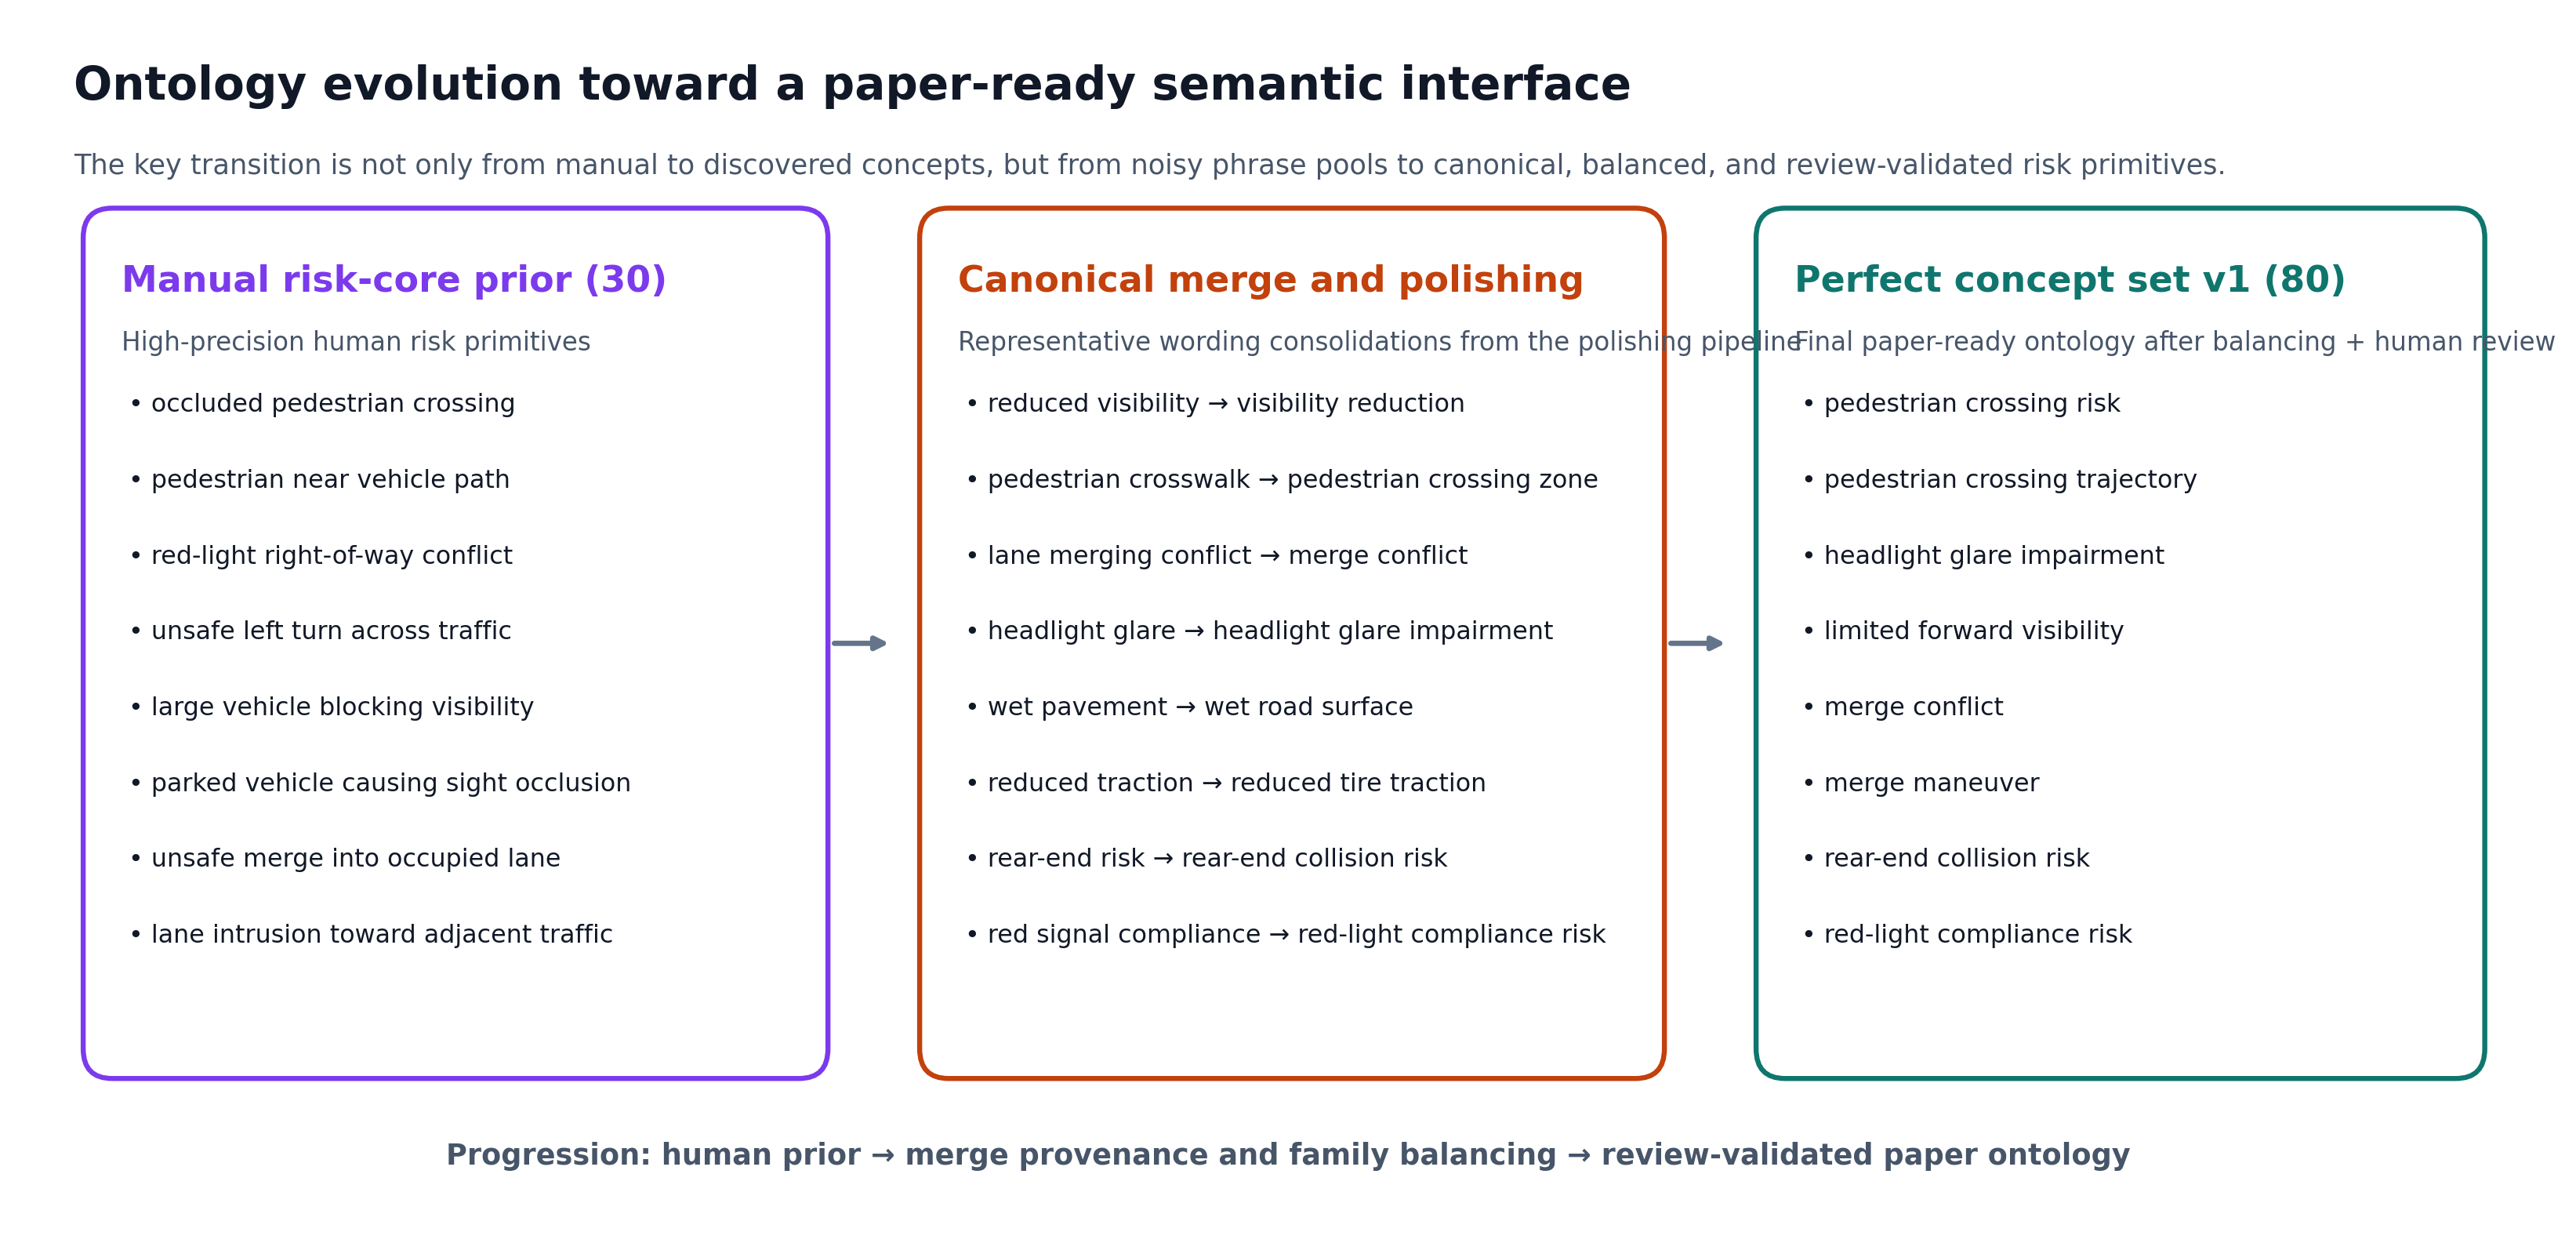
\includegraphics[width=0.98\textwidth]{../figures/insight_fig_concept_evolution.pdf}
  \caption{\textbf{Ontology evolution toward a paper-ready semantic interface.}
  Left: the manual risk-core ontology encodes strong human priors about accident
  precursors. Middle: representative merge and canonicalization examples from
  the polishing pipeline show how noisy or fragmented phrase clusters are
  compressed into stable risk primitives. Right: the final \emph{Perfect concept
  set v1} provides a balanced and review-validated ontology that is both more
  readable than the broad historical pool and more mature than early compact
  discovered pilots.}
  \label{fig:concept_evolution}
\end{figure*}

\begin{table}[t]
\caption{Concept ontology evolution across the project.}
\label{tab:concept_evolution}
\centering\small
\setlength{\tabcolsep}{4pt}
\resizebox{\linewidth}{!}{%
\begin{tabular}{lccp{0.42\linewidth}}
\toprule
Stage & \#Concepts & Source & Main property \\
\midrule
Historical full vocabulary & 837 & Broad CLIP-derived concept bank & High coverage, historically strongest CBM line, but semantically noisy and too large for clean paper presentation \\
Risk-core manual set & 30 & Manual risk-first curation & High-precision compact human prior over accident precursors \\
Perfect concept set v1 & 80 & Large-vocab discovery + polishing + human review & Balanced paper-ready ontology with canonical naming, merge provenance, explicit family coverage, and exhaustive per-concept review \\
\bottomrule
\end{tabular}%
}
\end{table}

\paragraph{Controlled ontology block status.}
The shared-launcher ontology comparison described in the main paper is now
complete as an artifact block: all six recommended runs
(\texttt{DAD/A3D} crossed with \texttt{historical\_full},
\texttt{risk\_core\_v1}, and \texttt{perfect\_v1}) are present with stored
checkpoints and \texttt{results.json} summaries. This matters because the
ontology claim is no longer resting on planned compute. On DAD, the compact
manual ontology achieves the highest AP while the polished discovered ontology
achieves the best mTTA; on A3D, the polished ontology achieves the strongest AP
while the compact manual ontology gives the best timing metrics. In other
words, the appendix now supports the main-paper reading directly: ontology
choice changes the operating point under one matched recipe.

The seed-backed extension of this block is also complete: all $18/18$
recommended seeded ontology runs have finished. This matters because the
ontology claim no longer depends on a half-completed follow-up.
The aggregate picture is consistent with the main paper's interpretation. On
A3D, the polished discovered ontology remains a strong AP-oriented operating
point under three seeds ($93.35\%\pm0.49$ AP), while on DAD the same ontology
is visibly more variable ($60.11\%\pm7.40$ AP). We therefore read the multi-seed
results as strengthening the ontology-science claim while also sharpening the
paper's limitation statement: the semantic interface looks materially more
stable on A3D than on DAD.

\paragraph{Prompt template design.}
Our prompts explicitly instruct the multimodal model to prioritise
\emph{safety-relevant early cues} rather than generic scene description.
Representative output fields include a compact concept phrase, a short risk
rationale, and a semantic family tag. A simplified prompt sketch is:
\begin{quote}
``Given a pre-crash driving frame, list short risk concepts that could function
as accident precursors. Prefer dynamic hazard cues, proximity conflict,
visibility degradation, braking or cut-in behaviour, and lane-level conflict.
Avoid generic objects or background scene tags unless they directly contribute
to accident risk.''
\end{quote}
We pair this instruction with a structured JSON schema so that outputs can be
programmatically filtered, clustered, and adjudicated. A representative schema
fragment is shown below.

\begin{quote}
\small
\noindent\parbox{0.95\linewidth}{\raggedright\ttfamily
\{"frame\_id": "dad\_xxx\_f042",\\
"risk\_concepts": [\\
\hspace*{1em}\{"concept": "trajectory conflict",\\
\hspace*{2em}"family": "motion\_conflict",\\
\hspace*{2em}"why\_risky": "vehicles are converging into\\
\hspace*{2em}the same path"\},\\
\hspace*{1em}\{"concept": "forward visibility limit",\\
\hspace*{2em}"family": "visibility",\\
\hspace*{2em}"why\_risky": "driver cannot reliably\\
\hspace*{2em}anticipate hidden hazards"\}\\
],\\
"discarded\_scene\_tags": ["road", "car", "intersection"]\\
\}}
\normalsize
\end{quote}

\paragraph{Concrete examples from the current polishing pipeline.}
The manual risk-core set contains phrases such as \emph{lane intrusion toward
adjacent traffic}, \emph{oncoming-traffic conflict}, and \emph{large vehicle
blocking visibility}. The newer large-vocabulary discovery stage produces a
much broader phrase pool that includes many useful but fragmented variants,
such as \emph{reduced visibility}, \emph{pedestrian crosswalk},
\emph{lane merging conflict}, or \emph{wet pavement}. The polishing stage then
consolidates these into canonical training-ready forms such as
\emph{visibility reduction}, \emph{pedestrian crossing zone},
\emph{merge conflict}, and \emph{wet road surface}. Including both raw and
canonical forms is important: it shows how the pipeline moves from high-recall
multimodal phrase mining toward a smaller, more stable, and more reviewable
ontology without losing the underlying risk semantics.

\paragraph{Failure modes in raw discovery.}
The raw discovery stage is intentionally high recall and therefore noisy.
Typical failure modes include: (i) generic object mentions that carry little
predictive value (e.g., ``road'', ``vehicle''), (ii) visually salient but weakly
risk-relevant background phrases, (iii) duplicate concepts with slightly different
wording, and (iv) over-specific phrases that do not transfer across clips.
These failure modes are precisely why the refinement and adjudication stages
are necessary; they are not implementation accidents, but expected properties
of an intentionally recall-heavy front end.

\paragraph{Why polishing plus human review is useful.}
The final ontology stage does more than clean spelling. It rebalances semantic
families, collapses near-synonyms, enforces canonical naming, and applies a
very-light human review over every retained concept. This matters for both
science and engineering: the method needs a reproducible ontology with visible
provenance, and the downstream model wants a small set of stable concepts
rather than a fragile bag of aliases. Figure~\ref{fig:concept_case_study} shows
representative real merge examples from this process, moving from noisy raw
multimodal phrases to final canonical concepts that can be presented in the
paper and used directly for downstream CBM training.

The current audit trail makes this concrete. Starting from 611 mined phrases,
the polishing pipeline compresses the pool to 81 post-polish canonical
candidates and a finalized paper release of 80 retained concepts. The review
record spans all 80 retained concepts across nine semantic families, and the
documented decisions are intentionally light-touch: wording is checked and
canonicalized, but the ontology is not rebuilt by hand. This is the level of
governance we want the paper to claim: explicit canonical naming, visible merge
provenance, and family balance that can be inspected by a reader without
pretending that the vocabulary is a finished standalone linguistic resource.

\paragraph{What the language-side evidence is meant to establish.}
The paper does not claim that these canonical names are universally optimal or
that the ontology has become a finished linguistic resource. The narrower and
more defensible claim is that the ontology is governed enough to function as a
scientific interface: canonical names remain reasonably stable under light
paraphrase variation, semantic families are explicit rather than implicit, and
merge choices are reviewable rather than hidden inside prompt iteration.

\begin{figure*}[t]
  \centering
  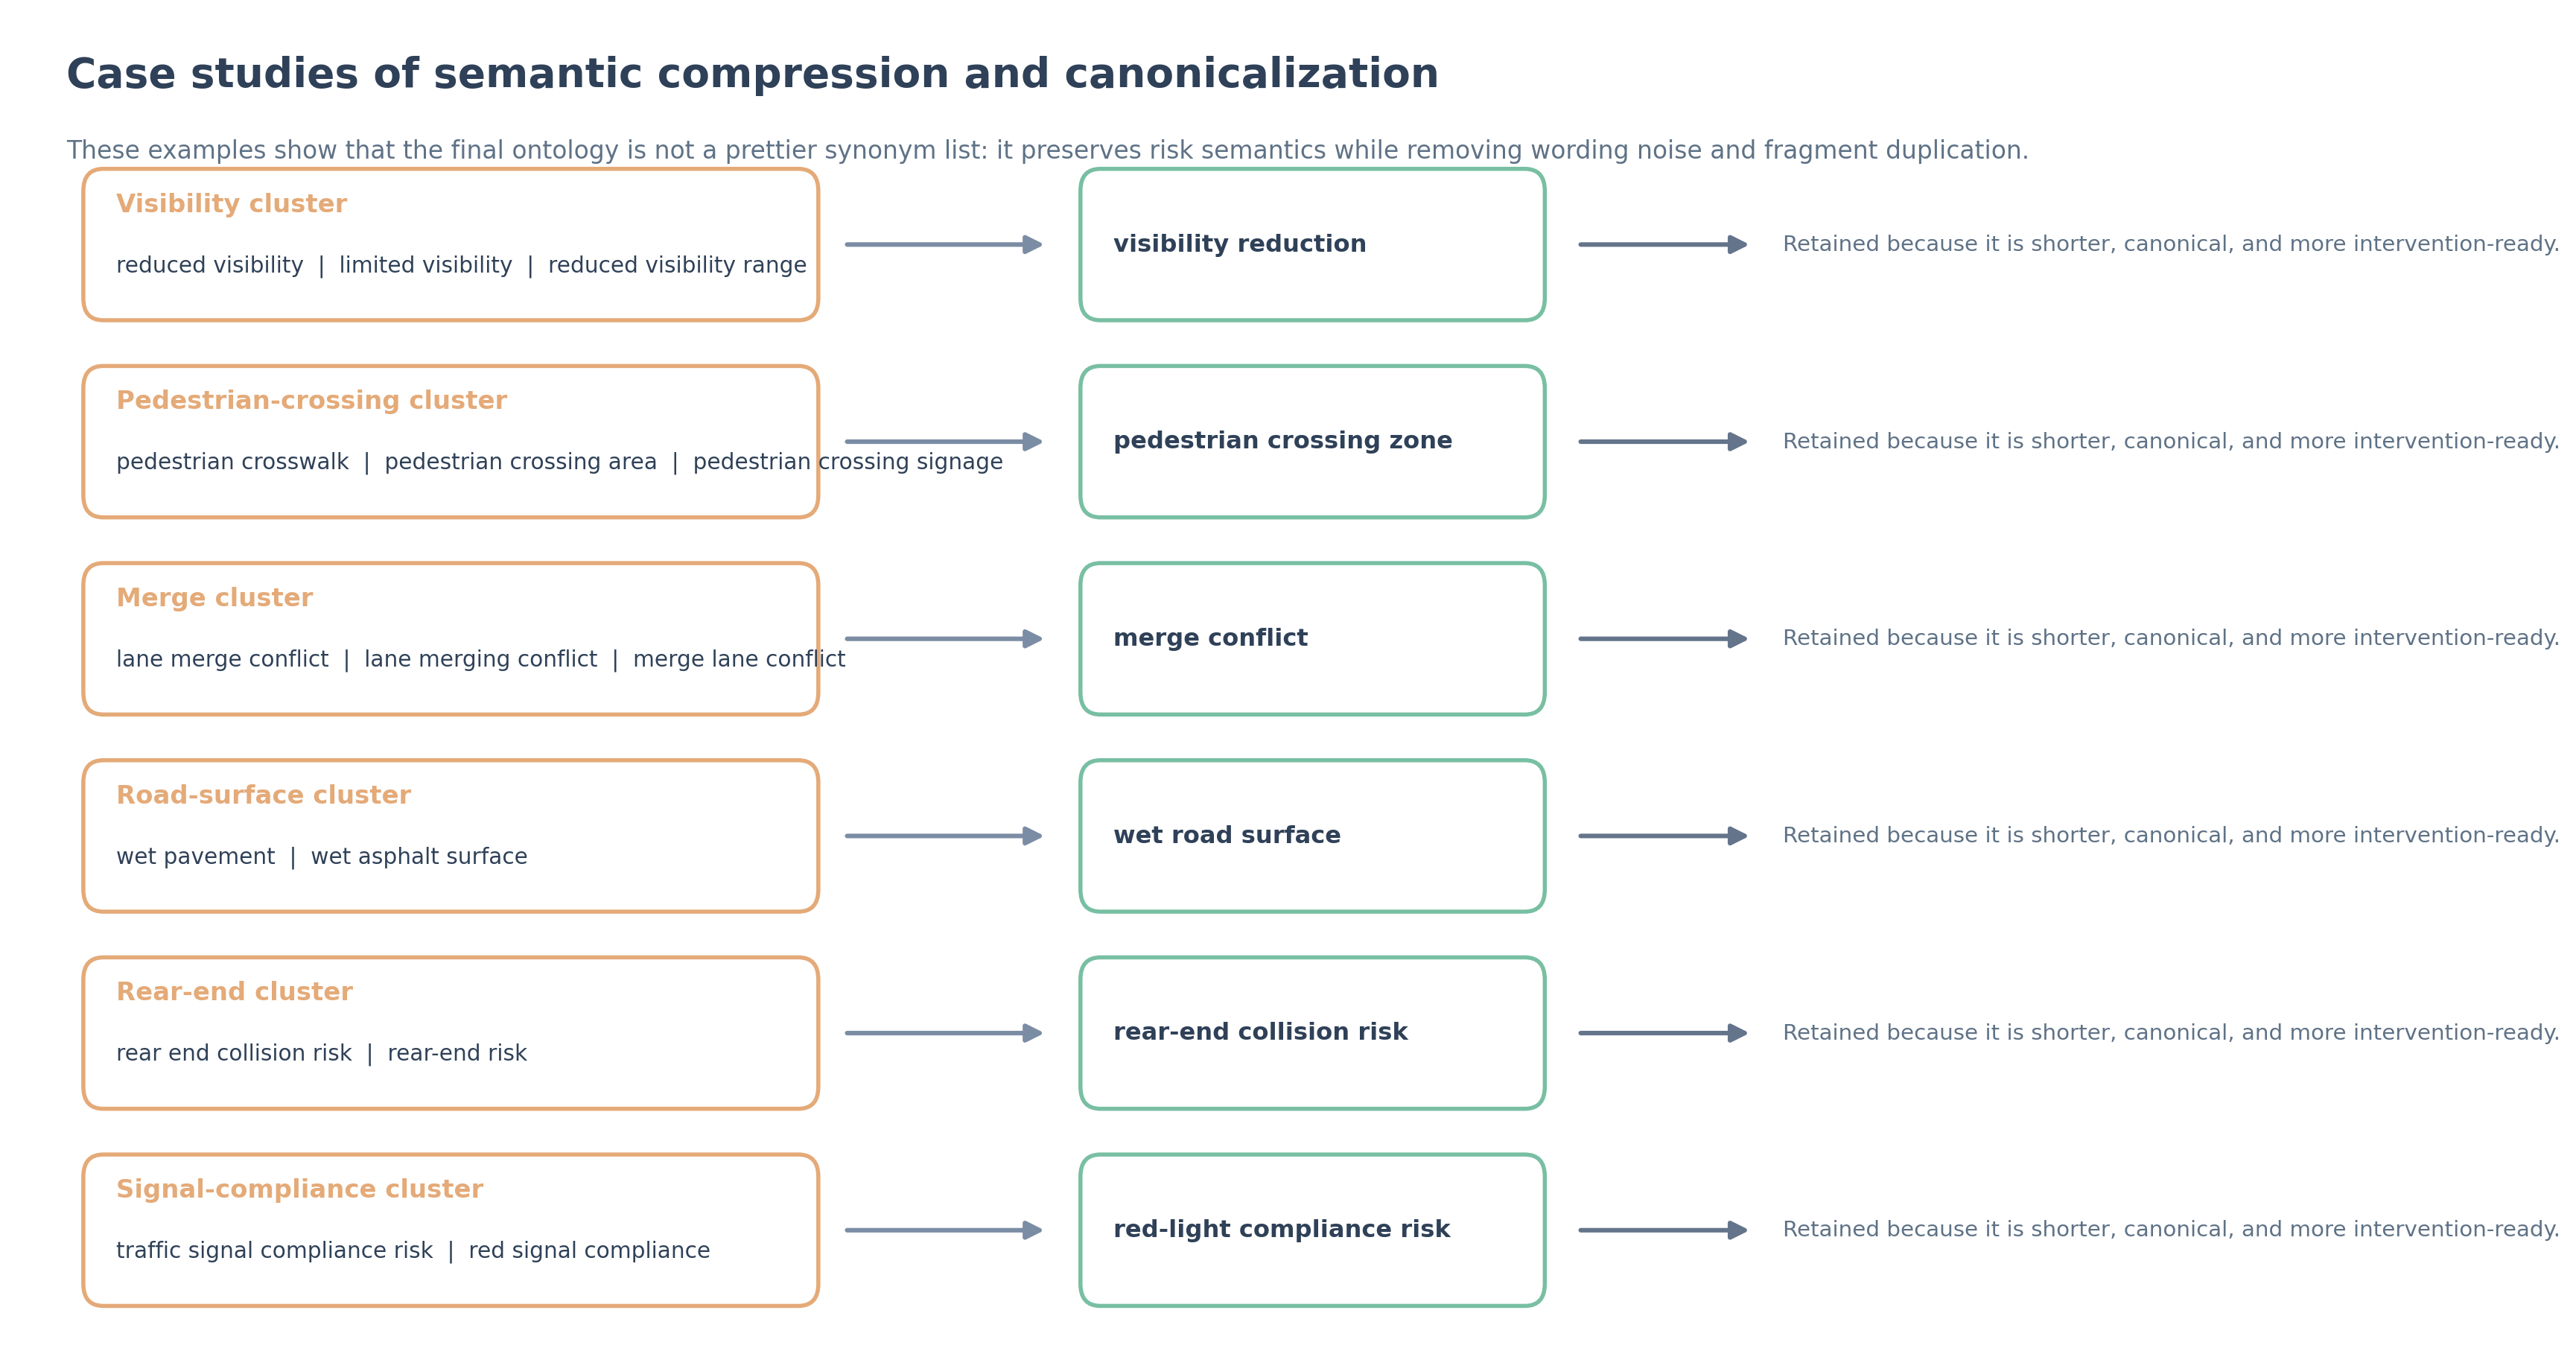
\includegraphics[width=0.98\textwidth]{../figures/insight_fig_concept_case_study.pdf}
  \caption{\textbf{Case studies of semantic compression and canonicalization.}
  Each row shows a representative merge path from noisy or fragmented phrase
  variants to a single canonical paper-ready concept. These examples make two
  points explicit: the pipeline removes lexical fragmentation, and the final
  ontology is not merely a prettier synonym list but a more stable semantic
  interface for downstream CBM training, family-level analysis, and external
  auditing.}
  \label{fig:concept_case_study}
\end{figure*}

\paragraph{What counts as success.}
A discovered concept set is successful only if it satisfies four criteria:
(1) semantic plausibility to a human reader, (2) coverage of major accident
precursor families, (3) trainability in the downstream CBM pipeline, and
(4) auditability at the paper level through family metadata, merge provenance,
and human review. This is why the paper reports not only ontology examples and
downstream training results, but also family-balance figures and merge case
studies. A pretty concept list without learning value is not enough; conversely,
a trainable but uninterpretable list would defeat the purpose of the semantic
interface.

\begin{figure}[t]
  \centering
  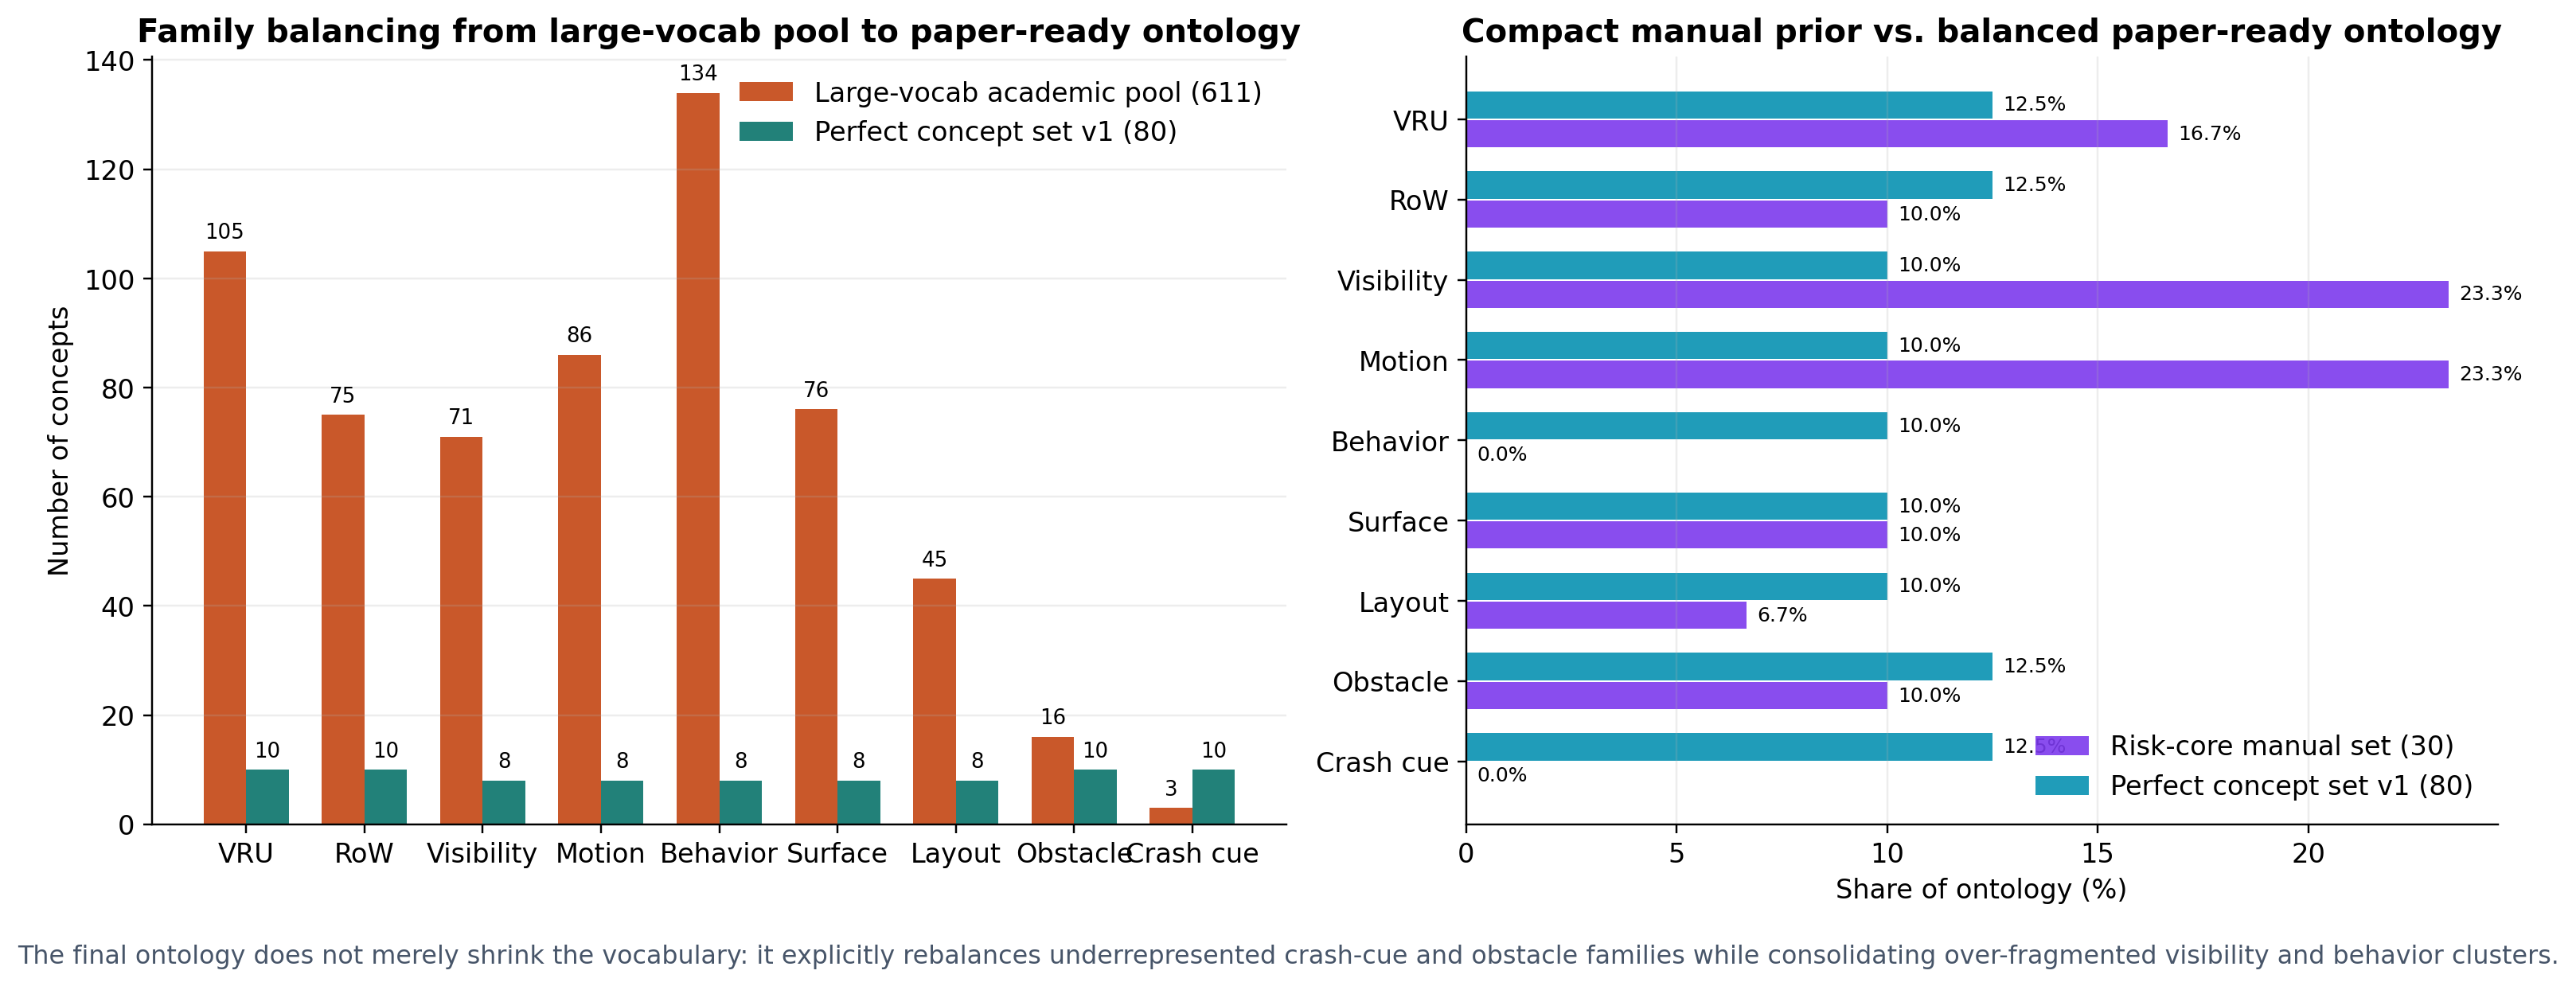
\includegraphics[width=0.98\linewidth]{../figures/insight_fig_concept_family_coverage.pdf}
  \caption{\textbf{Family coverage before and after ontology polishing.}
  The broad large-vocabulary pool is highly imbalanced, while the final paper-ready
  ontology explicitly rebalances crash-cue, obstacle, and vulnerable-road-user
  families without collapsing the ontology into a tiny manually curated list.
  This supports our claim that ontology polishing is not cosmetic compression;
  it is a structured operation that improves auditability and semantic balance.}
  \label{fig:concept_family_coverage}
\end{figure}

\subsection{Why the Semantic Interface Can Affect Timing}
\label{app:theory}

\paragraph{From latent prediction to semantic decision-making.}
A conventional recurrent anticipation model compresses all evidence into a
single latent state $\mathbf{h}_t$ and predicts risk from that state alone.
This is often sufficient for raw prediction, but it is weak from an auditing
perspective because the model offers no explicit separation between
\emph{evidence extraction} and \emph{decision timing}. By contrast, \method{}
explicitly decomposes these two roles:
\begin{itemize}[leftmargin=1.5em]
  \item the \textbf{semantic layer} estimates a concept state $\mathbf{c}_t$ that
  summarises semantically meaningful risk evidence, and
  \item the \textbf{timing layer} learns a timing policy over a concept-aware
  sequential state $\mathbf{s}_t=[\mathbf{h}_t\|\mathbf{c}_t]$.
\end{itemize}
This decomposition is not cosmetic. It changes the information geometry of the
problem: the policy no longer acts on an opaque hidden vector alone, but on a
state with an explicit semantic interface.

\paragraph{A simple monotonicity view.}
Suppose the concept state contains one or more dimensions corresponding to
hazard indicators whose increase is semantically consistent with increasing
risk. If the downstream timing policy is trained to reward earlier correct
alerts, then a policy conditioned on $\mathbf{s}_t=[\mathbf{h}_t\|\mathbf{c}_t]$
can, in principle, cross the alert boundary before a purely confidence-based
predictor reaches its peak. Informally, the concept channel acts as an early
warning basis: a rise in concept evidence can move the system toward action
before the latent classifier has accumulated maximal confidence. This is the
core reason the semantic and timing layers are coupled but not redundant.

\paragraph{Why intervention is meaningful.}
Let a concept edit be represented as a perturbation
$\Delta\mathbf{c}_t$ applied over a short pre-crash window.
Because the downstream predictor or policy consumes a state containing the
concept vector, the perturbation induces a corresponding perturbation in the
decision state:
\[
\mathbf{s}'_t = [\mathbf{h}_t\|\mathbf{c}_t + \Delta\mathbf{c}_t].
\]
If the architecture is truly concept-conditioned rather than merely
post-hoc-explainable, then semantically valid positive perturbations on a risk
concept should induce a stronger or earlier warning response at the output.
This is why the intervention analysis is an architectural test, not just a
visualisation trick. The test asks whether the semantic interface has
non-trivial structured influence on the decision pathway.

\paragraph{What this appendix-level analysis does and does not claim.}
We do not claim a formal global theorem guaranteeing monotone policy shifts for
all concept edits, since the recurrent dynamics and nonlinearities are too rich
for such a guarantee to be informative without unrealistic assumptions. The
point of the analysis is instead to make clear why the design is principled:
separating semantic evidence estimation from timing control creates a decision
pathway that is inspectable, perturbable, and therefore much closer to the
needs of safety auditing than a single black-box recurrent score.

\subsection{Scoped Intervention Evidence}
\label{app:intervention}

A standard promise of concept bottleneck models is \emph{intervenability}: a
human can inspect a concept, judge that it is mis-estimated, and correct it
without retraining the full network. For accident anticipation, this capability
is especially important because many practically relevant errors are not
arbitrary; they are tied to under-activation of an intuitively correct risk
concept. In the current paper, however, intervention should be read as
\emph{support evidence} for a meaningful semantic control surface, not as a
completed policy-level causal benchmark.

\begin{figure*}[t]
  \centering
  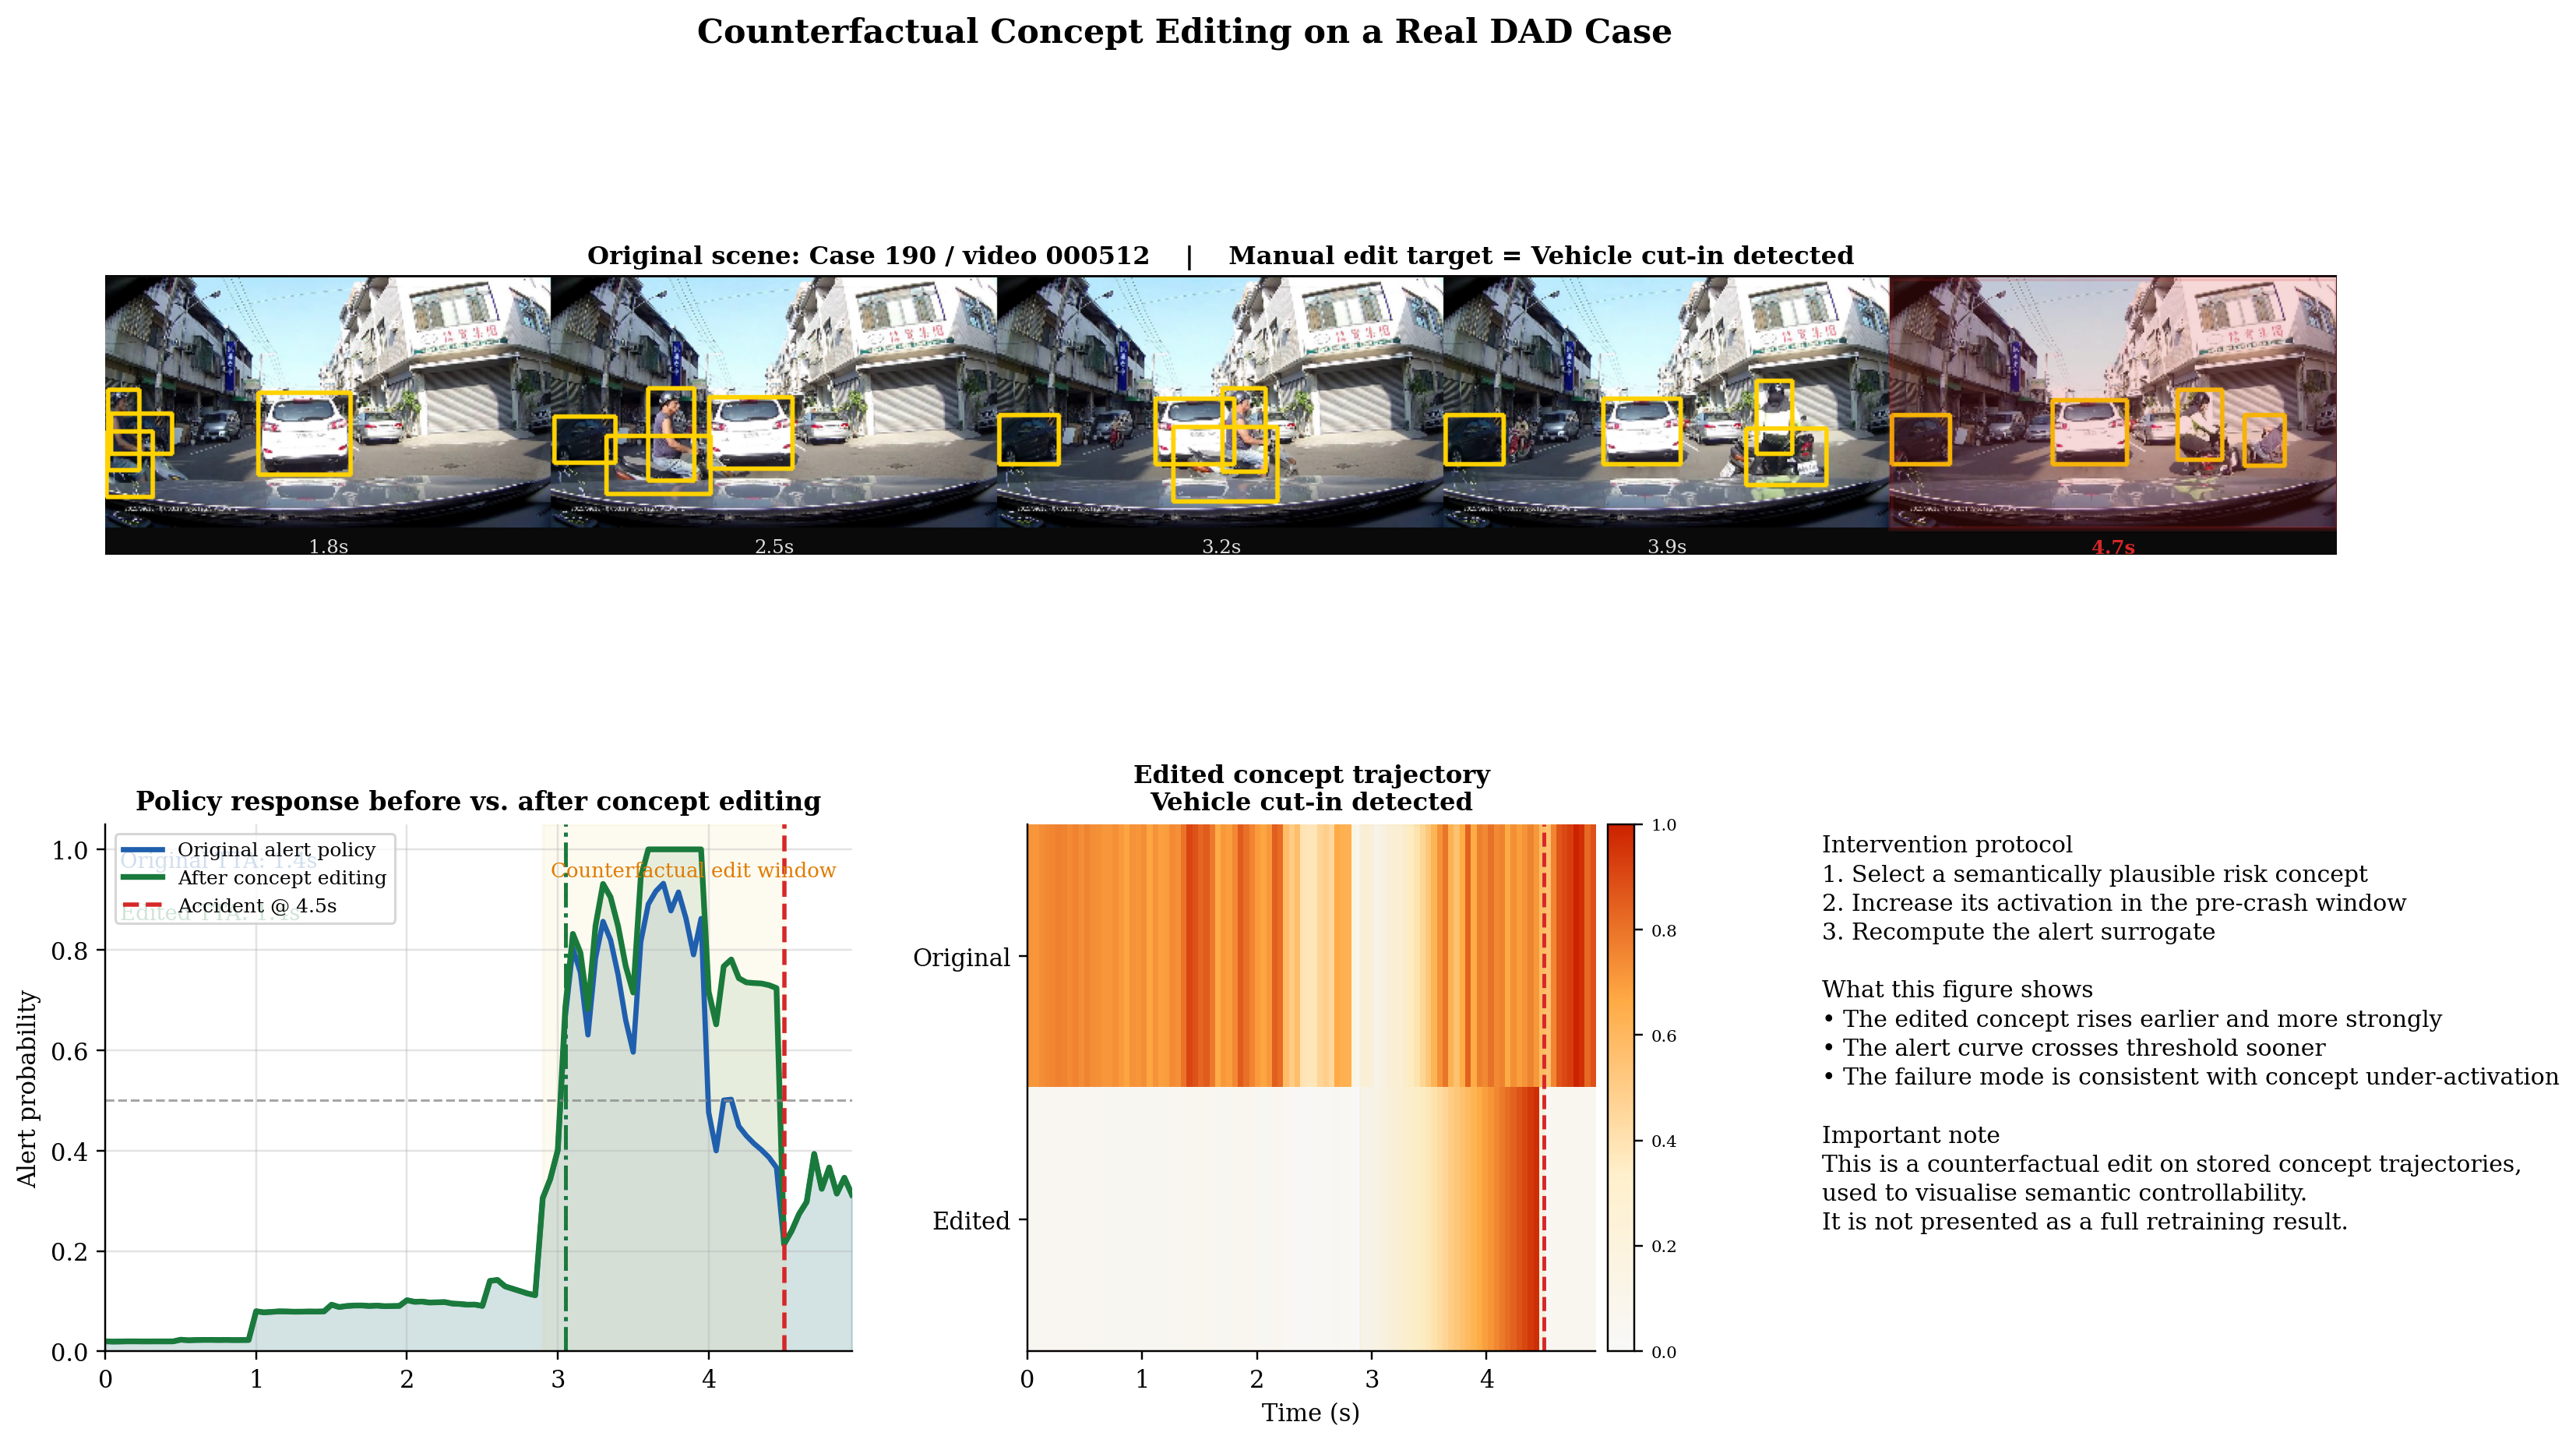
\includegraphics[width=\textwidth]{../figures/insight_fig_appendix_intervention.pdf}
  \caption{\textbf{Counterfactual concept editing on a DAD case.}
A semantically plausible pre-crash concept trajectory is increased and the
resulting warning surrogate is recomputed. The edited concept rises earlier,
and the alert curve crosses threshold sooner. This figure is intentionally a
stored-trajectory counterfactual rather than a full model re-run; its role is
to show that the model exposes a semantically meaningful control surface.}
  \label{fig:appendix_intervention}
\end{figure*}

\paragraph{Stored-trajectory intervention protocol.}
For a false-negative or borderline DAD case, we select a concept whose
activation is visibly inconsistent with the scene semantics, increase it over
the pre-crash window, and compare the original and edited warning trajectories.
This directly tests whether strengthening the right concept can move the
warning earlier.

\paragraph{Outcome.}
Figure~\ref{fig:appendix_intervention} shows that it can. The edited alert
curve rises and crosses threshold earlier than the original one. Across the
archived quantitative summaries, however, the effect remains heterogeneous. In
the strongest archived hybrid-boost setting, the mean alert shift is
$-2.04$ frames over 64 cases, but the median shift is still 0.0; by contrast,
both the null-style hybrid baseline and the risk-weight baseline produce a mean
shift of 0.0 over 32 cases each. The correct interpretation is therefore
\emph{partial structural intervenability} rather than a completed causal proof.

\begin{figure*}[t]
  \centering
  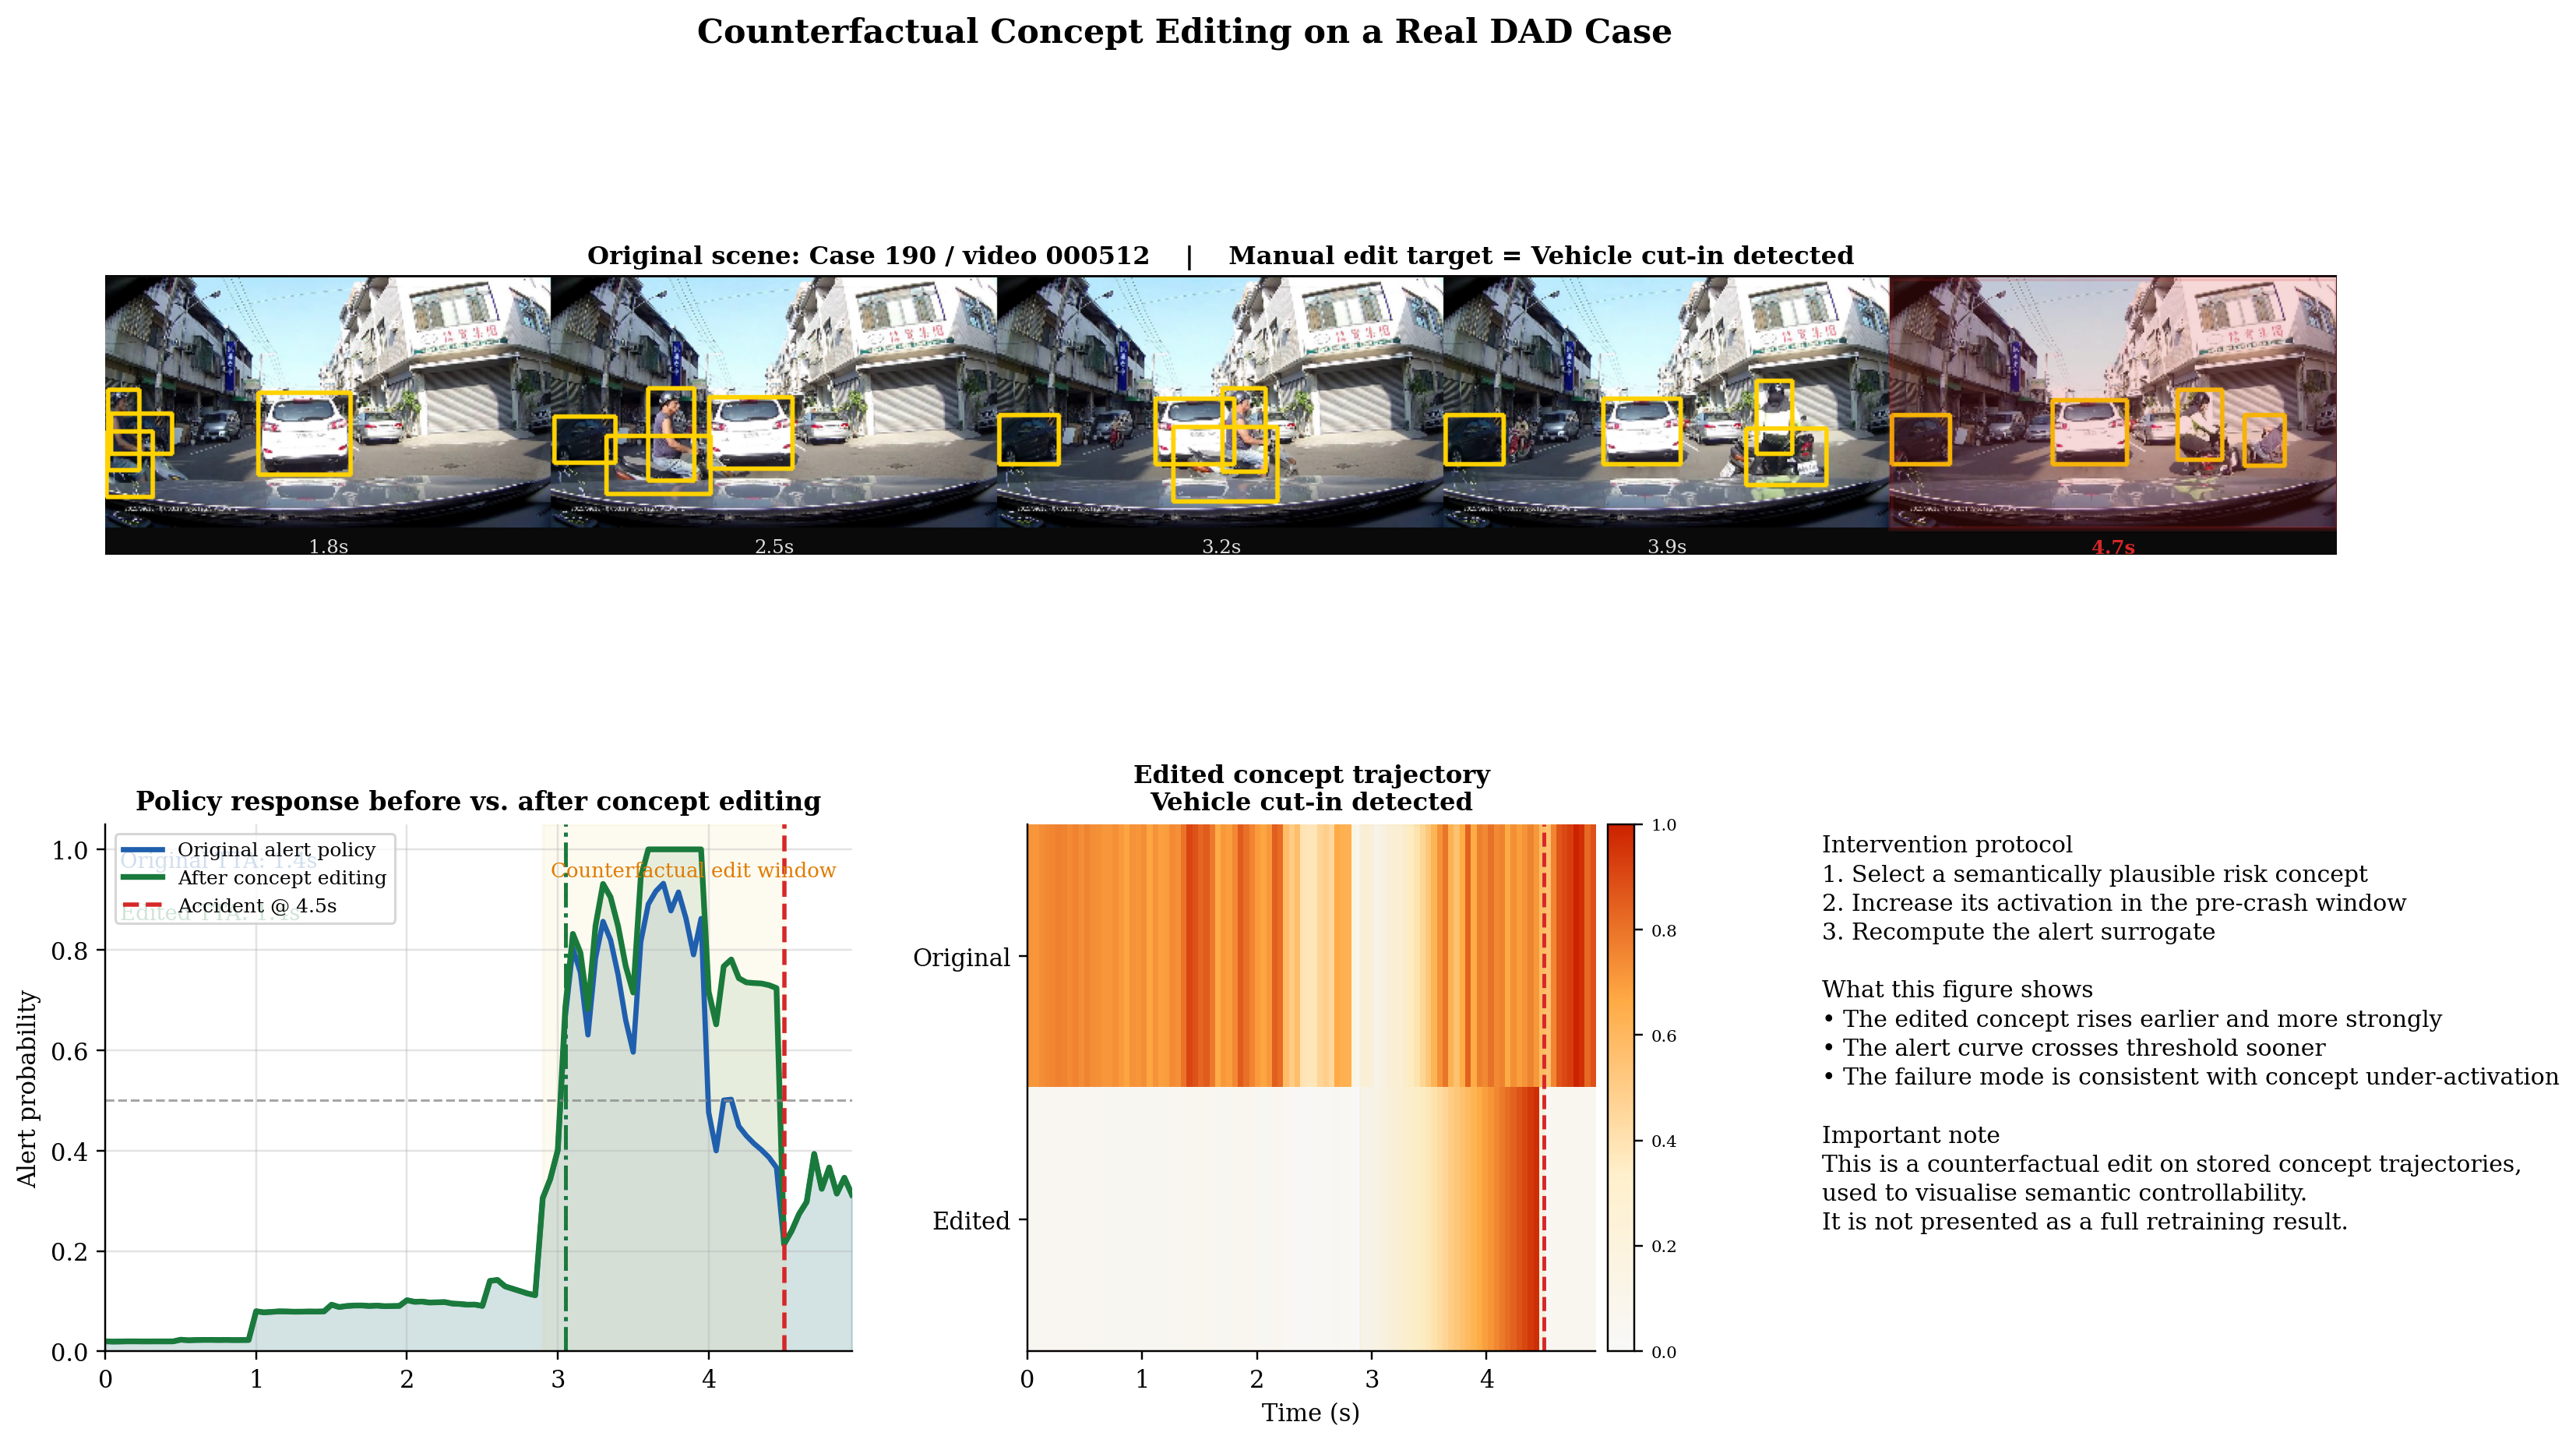
\includegraphics[width=\textwidth]{../figures/insight_fig_appendix_intervention_v4_backbone.pdf}
  \caption{\textbf{Backbone-level intervention re-run with the v4 DAD checkpoint.}
A concept channel is edited in the pre-crash window and the downstream
prediction branch is recomputed through the loaded backbone. This is a stronger
intervention path than stored-trajectory editing, but it is still not a full
policy-level intervention because the available checkpoint lacks the final
Actor--Critic head weights.}
  \label{fig:appendix_intervention_v4}
\end{figure*}

\paragraph{Backbone-level re-run.}
To go beyond stored-trajectory editing, we also run a backbone-level
intervention using the newer DAD line. The available checkpoint loads the
concept bottleneck, temporal modules, and recurrent backbone, but not the final
Actor--Critic head weights. We therefore edit one concept channel and recompute
the downstream prediction branch through the loaded backbone.

\paragraph{Interpretation.}
The backbone-level re-run shows that concept edits remain meaningful when
propagated back through the loaded model rather than only visualised post hoc.
It also makes the current evidence boundary explicit: we can support a
concept-conditioned backbone intervention, but not yet a full policy-level
intervention without the complete Actor--Critic checkpoint.

\paragraph{Backbone-level search as a robustness check.}
To test whether Figure~\ref{fig:appendix_intervention_v4} was unusually
favourable, we also ran an automatic search across positive DAD test cases
available to that checkpoint line. For each case, we selected several
high-activity pre-crash concepts, applied graded positive edits over the
pre-crash window, and re-ran the backbone-level prediction branch. The result
is best read as an intermediate intervention audit: concept edits can propagate
through the loaded model and sometimes move warning behaviour in the expected
direction, but they do not yet support a broad claim of large or reliable
timing gains across DAD. This conclusion is reinforced by the scan artifacts:
the best stored v4 search cases mostly show no TTA improvement at all, even
when peak prediction scores shift slightly.

\subsection{Additional Qualitative Analysis}
\label{app:qual}

\begin{figure*}[t]
  \centering
  
\includegraphics[width=0.84\textwidth]{../neurips2026/dad_case_contactsheet.pdf}
  \caption{\textbf{A broader DAD case bank for qualitative screening.}
  Positive DAD test cases were ranked by a simple combination of peak risk,
  pre-crash area, and rise strength, then reviewed for visual legibility.
  The contact sheet spans different traffic geometries and visibility
  conditions, reducing the chance of a single unusually clean case driving the
  qualitative story.}
  \label{fig:appendix_casebank}
\end{figure*}

The main paper intentionally keeps the qualitative section compact. Here we
summarise the broader qualitative patterns observed across DAD cases.

\paragraph{Empirical summary of the appendix case bank.}
Taken together, the contact-sheet screening and the intervention analysis show
that the semantic interface is visible across multiple DAD scenes rather than
only in a single clean success case. At the same time, the v4 backbone search
shows that stronger concept edits do not automatically translate into large
timing shifts in every case. The appendix therefore supports both breadth of
semantic evidence and a realistic boundary on controllability.

\paragraph{Hard-case symmetry audit snapshot.}
To avoid overclaiming from qualitative examples, we maintain a separate
family-level hard-case symmetry scaffold
(`paper/neurips2026/dad_hard_case_symmetry_audit.md`) generated from archived
casebank assets. Table~\ref{tab:appendix_hard_case_symmetry} reports the
current snapshot using a primary-family heuristic and prediction-branch timing
buckets. The table is intentionally conservative: it is an audit checkpoint,
not a claim that symmetry is solved.

\begin{table}[t]
\caption{DAD hard-case symmetry audit snapshot from archived v4 casebank assets.
Counts are from the current `strong_top` pool under primary-family assignment.
`auto\_pair` denotes heuristic early-vs-late mixed pair suggestions that still
require manual reviewer confirmation.}
\label{tab:appendix_hard_case_symmetry}
\centering\small
\begin{tabular}{lrrrr}
\toprule
Primary family & Early strong & Early marginal & Late/missed & Auto pair \\
\midrule
intersection\_merge & 1 & 3 & 10 & 4 \\
visibility\_night & 0 & 0 & 6 & 0 \\
pedestrian\_conflict & 0 & 0 & 7 & 0 \\
road\_surface\_weather & 0 & 0 & 2 & 0 \\
heavy\_vehicle\_conflict & 0 & 0 & 1 & 0 \\
\bottomrule
\end{tabular}
\end{table}

This snapshot reinforces the same scope boundary used in the main paper:
current synchronized diagnostics and archived casebank evidence reveal uneven
hard-case behavior, so stronger symmetry claims remain blocked until manual
pair-level outcomes are completed in the audit file.

\begin{figure*}[t]
  \centering
  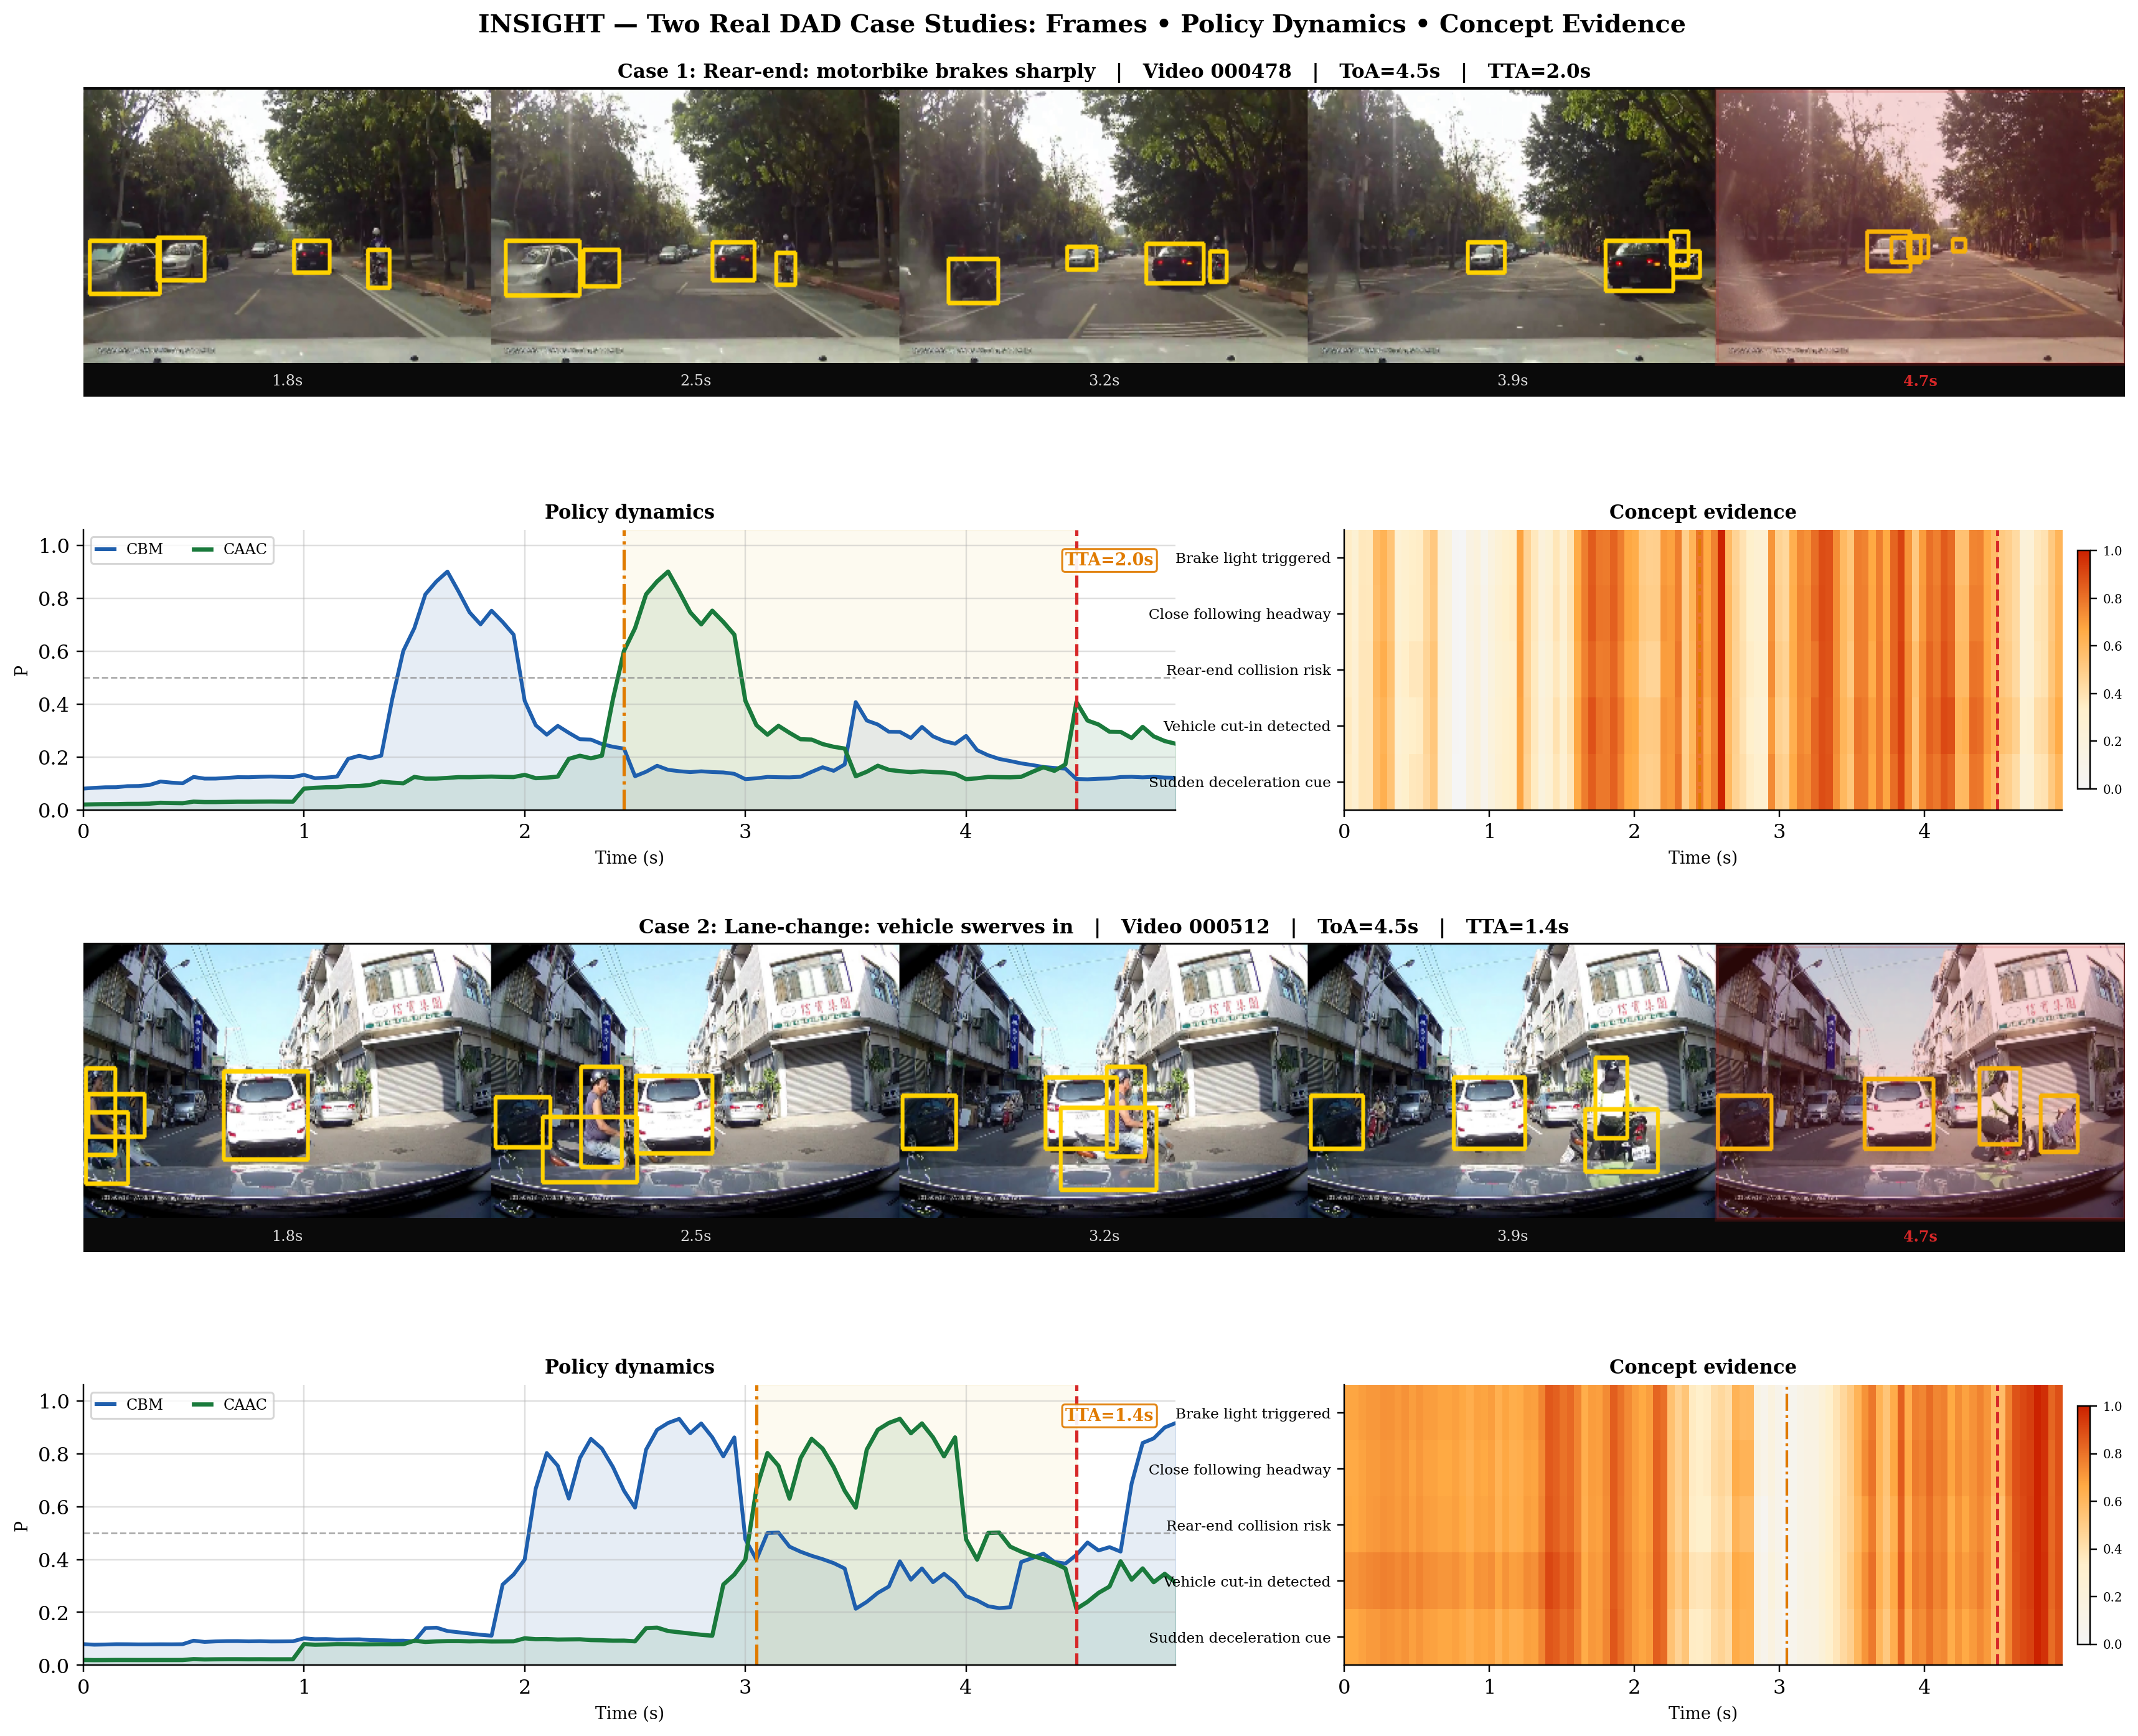
\includegraphics[width=0.98\textwidth]{../figures/insight_fig_appendix_v4_casebank_selected.pdf}
  \caption{\textbf{Selected v4 DAD cases ranked by prediction-branch behaviour.}
  Using the runnable v4 checkpoint, we extract a shortlist containing an
  earlier-warning case, near-threshold borderline cases, and a harder
  low-visibility example. Because the alert surrogate is nearly flat on this
  checkpoint line, the figure should be read as a prediction-level qualitative
  bank rather than as a policy-level alert benchmark.}
  \label{fig:appendix_v4_casebank_selected}
\end{figure*}

\paragraph{Case diversity.}
Across rear-end, lane-change, and intersection scenarios, the dominant
concepts change substantially, but the qualitative pattern stays similar: the
\cbm{} surfaces plausible risk factors first, and the downstream timing signal
responds as those factors rise. The appendix figures also show that visually
strong cases vary in difficulty, from clean agent separation to cluttered or
low-visibility scenes.

\paragraph{Policy-before-peak behaviour.}
In selected qualitative figures, the green \caac{} curve can cross its alert
threshold \emph{before} the blue raw accident-probability curve peaks. This is
consistent with the intended effect of the time-remaining reward: the timing
consumer can respond to a rising semantic trend rather than waiting for maximal
confidence. We present this as qualitative support for the design, not as a
standalone policy benchmark.

\paragraph{Frame--concept alignment.}
The strongest visual evidence occurs when a concrete scene change is mirrored
by a concept change: brake lights activate, headway shrinks, or a vehicle cuts
into the ego lane, and the corresponding concept rows intensify in the
heatmap. Not every high-scoring sample is equally legible, which is why case
selection matters for qualitative presentation.

\subsection{Failure Modes, Robustness Considerations, and Dataset-Specific Discussion}
\label{app:failure}

\paragraph{Low-visibility conditions.}
Night-time and poor-weather scenes remain challenging. In these settings, the
ROI features are weaker and concept activations become less reliable,
especially for fine-grained cues such as brake lights or subtle lane-boundary
signals. The resulting failure mode is usually concept under-activation rather
than an obviously incorrect timing policy.

\paragraph{Crowded scenes.}
When many agents are present simultaneously, the object-focused aggregation
must compress a large amount of interaction structure into a fixed hidden
state. This can dilute the representation of the single most critical risk
agent. A natural next step is a more explicit risk-agent selection mechanism
layered on top of the concept bottleneck.

\paragraph{Concept vocabulary coverage.}
Although 837 concepts provide broad coverage, rare corner cases still exist
where the needed concept is absent or too coarse. This is a limitation of any
finite concept vocabulary. Future work could investigate adaptive or
hierarchical concept sets that retain auditing benefits while improving
long-tail coverage.

\paragraph{Why A3D and DAD behave differently.}
The qualitative evidence suggests that the relative value of semantic
structuring is dataset-dependent. In A3D, many hazards develop progressively,
so early concept growth is especially useful for anticipation. DAD is harsher:
the margin between weak early signal and crash onset is smaller, and the scenes
are often more cluttered. This likely explains why DAD is both a harder
benchmark and a more sensitive test of concept reliability.

\paragraph{Robustness interpretation.}
The main robustness point is that the semantic interface remains useful across
multiple datasets and accident types even when controllability is not uniformly
strong across all checkpoints and scenes. The v4 appendix search therefore
serves as prediction-level qualitative support rather than as a policy-level
ranking result.
accident anticipation should be treated as a concept-conditioned sequential
decision problem, not merely as frame-wise classification with post-hoc
explanation.


\clearpage
\bibliographystyle{plainnat}
\bibliography{insight}

\clearpage
\input{checklist}

\end{document}
